\chapter{Double Higgs Bosons Production Analysis}
\label{chap:DoubleHiggs}

\chapterquote{The supreme art of war is to subdue the enemy without fighting.}%
{Sun Tzu, 544 BC-496 BC}%: Blackwood's Magazine May 1830


Since the discovery of Higgs boson at the \LHC in 2012\cite{Aad:2012tfa,Chatrchyan:2012ufa}, it is crucial to understand the properties of the Higgs boson and test if it is a Standard Model Higgs. A number of theories beyond the Standard Model may be tested via the double Higgs production in an electro-positron collider (see \Section{sec:theoryHiggsBSM}). Generator level studies have shown that the precision reached by a multi-TeV linear collider, such as the Compact Linear Collider (\CLIC), is superior to that of the Large Hadron Collider (\LHC) and high luminosity upgraded \LHC  \cite{Contino:2013gna}.

%The Higgs mechanism and the Higgs boson in the Standard Model have been explained in \Chapter{chap:Theory}. even with 3000$fb^{-1}$ of data

The first challenge for the double Higgs bosons production analysis is the cross section(0.149\,fb at \rootS{1.4} and 0.588\,fb at \rootS{3}) is very small compared to background processes, making it difficult to select signal events. The second challenge is that at high centre-of-mass energies, events are boosted and many final-state particles are in the forward region of the detector, where the reconstruction performance is inferior to the barrel region and particles can escape detection.

In this chapter, a full \CLICILD detector simulation study has been performed for the double Higgs production, \eeToHH, via \WW fusion. Event generation and simulation will be discussed first. An overview of the analysis, including lepton finding and jet reconstruction, is presented, followed by an optimised multivariate analysis to distinguish signal from background processes. The optimised event selection is used to derive an estimate of the potential for the \CLIC. The results of this analysis have been publish in \Reference{Abramowicz:2016zbo}.
%The results of the signal selection are interpreted in the context of the Higgs self coupling.

\section{Analysis Straggly Overview}

Leading-order Feynman diagrams for double Higgs production via \WW fusion are shown in \Figure{fig:doubleHiggsFeynman}. The diagram shown in the \Figure{fig:doubleHiggsFeynman1} contains a triple Higgs vertex, which is sensitive to Higgs triple self coupling \gHHH. The diagram in the \Figure{fig:doubleHiggsFeynman2} is sensitive to quartic coupling \gWWHH. \FIGURE{fig:doubleHiggsFeynman3} and \Figure{fig:doubleHiggsFeynman4} show the Feynman diagrams of irreducible background processes for the study of \gHHH and \gWWHH.


\begin{figure}[!htbp]
  \begin{subfigure}[b]{0.22\textwidth}
    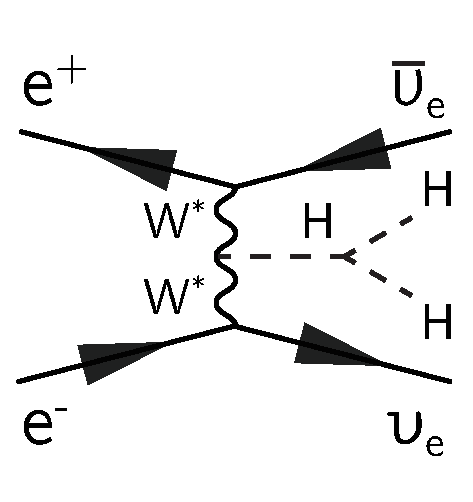
\includegraphics[width=\textwidth]{{{doubleHiggs/Feynman/1}}}
    \caption{}
    \label{fig:doubleHiggsFeynman1}
  \end{subfigure}
  \hfill
  \begin{subfigure}[b]{0.22\textwidth}
    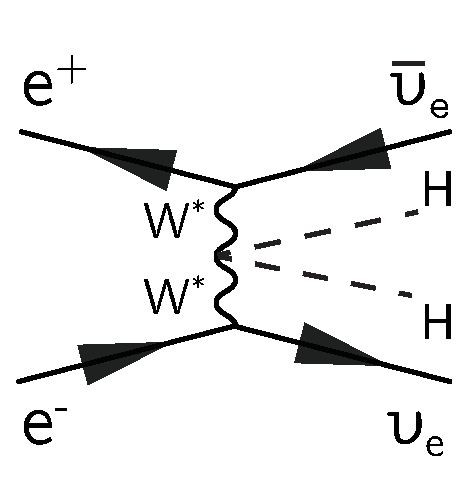
\includegraphics[width=\textwidth]{{{doubleHiggs/Feynman/2}}}
    \caption{}
    \label{fig:doubleHiggsFeynman2}
  \end{subfigure}
  \begin{subfigure}[b]{0.22\textwidth}
    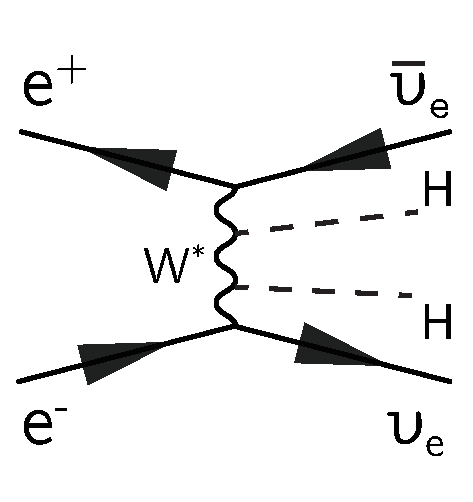
\includegraphics[width=\textwidth]{{{doubleHiggs/Feynman/3}}}
    \caption{}
    \label{fig:doubleHiggsFeynman3}
  \end{subfigure}
  \hfill
  \begin{subfigure}[b]{0.22\textwidth}
    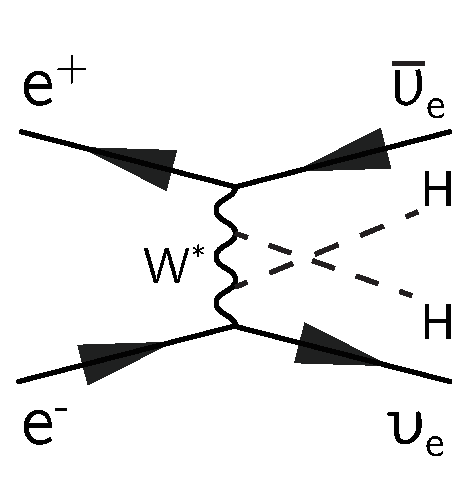
\includegraphics[width=\textwidth]{{{doubleHiggs/Feynman/4}}}
    \caption{}
    \label{fig:doubleHiggsFeynman4}
  \end{subfigure}
\caption
   {The main Feynman diagrams for the leading-order \eeToHH processes at the \CLIC.}
   \label{fig:doubleHiggsFeynman}
\end{figure}

Double Higgs production can be also produced via {\HepProcess{ \Pep \Pem \to \PZ \PHiggs \PHiggs}\xspace}, where \PZ decays to \HepProcess{\Pnu \APnu}. This \HepProcess{\PZ \PHiggs \PHiggs} channel has also been used to study at future \ee colliders, for example, the \ILC at \rootSGeV{500} \cite{Baer:2013cma}. However, for the relevant \CLIC energies at \rootS{1.4} and 3\,TeV, its contribution to the \HepProcess{\PHiggs \PHiggs \Pnu \APnu} final state is small compared to that of the \WW fusion, and can be neglected at the centre-of-mass energies in this thesis.

%The cross section of {\HepProcess{ \Pem \Pep \to \PZ \PHiggs \PHiggs}\xspace} is one order of magnitude smaller than \eeToHH via the \WW fusion,  shown in \Figure{fig:theoryHiggsCrossSection},. Therefore, the effect of {\HepProcess{ \Pem \Pep \to \PZ \PHiggs \PHiggs}\xspace} present in \eeToHH channel at \rootS{1.4} and 3\,TeV is negligible.


%However, {\HepProcess{ \Pem \Pep \to \PZ \PHiggs \PHiggs}\xspace} can be easily identified via the recoil mass. Hence {\HepProcess{ \Pem \Pep \to \PZ \PHiggs \PHiggs}\xspace} is not considered in this studied.

From an experimental prospective, \eeToHH production has several distinct final-state topologies. In this chapter, \eeToHHbbWW sub-channel  is investigated. Firstly the hadronic decay mode of the \eeToHHbbWW channel is chosen to study because the hadronic decay has the largest cross section and does not produce primary neutrinos, which allows each \PW to be reconstructed. The semi-leptonic final state is also considered. However, the neutrinos produced at the final states make it  difficult to reconstruct the two Higgs bosons, as some momenta of one Higgs boson is missing. This channel is discussed briefly and its analysis strategy is adapted from the hadronic decay analysis.
%The double Higgs production, \eeToHH, is divided into two sub-channel: \eeToHHbbWW and \eeToHHbbbb to target the specific kinematic properties if each final state, which provides cross-validation between two sub-channels and an improvement in signal selection when combined.


%However, hadronic decay final state of the \eeToHHbbWW has a very low cross section. The signal selection is challenging and aggressive background rejection methods are deployed.
The analysis of the \eeToHHbbbb  sub-channel has been studied independently by collaborators. In this thesis, two analyses are combined for the final couplings extractions.
%The    is studied independently by collaborators. However, there is collaboration between the two studies. The two analyses are combined on the final couplings extractions.

%Combining with the low cross section, results for these two final states are not reported. The analysis can be easily (and have been) adapted for the semi-leptonic and leptonic final states.

The process, \eeToHHbbWWHadFull, results in a six quark final state with missing momentum. The high number of quarks requires an efficient jet reconstruction and a jet pairing algorithm to select the signal. The two \Pbottom quarks in the final states can be identified statistically with \Pbottom jet tagging. %Since the final state does not contain leptons, event-level lepton finding - typically for energetic isolated leptons -  would improve the signal selection efficiency.

A proof-of-principle generator-level study has already been performed using the \CLICILD detector model for \rootS{1.4} and 3\,TeV\cite{Linssen:2012hp}. In this chapter a full \CLICILD detector simulation study is presented. Firstly, suitable signal and background channels are identified. In order to select the signal, events with primary lepton identified are vetoed.  Vertex information is used to identify \Pbottom quark jets. \PFOs in an event are then clustered into jets depending on the number of quarks in the final states. Events selected based on this jet assignment are then used for pre-selection and multivariate analysis. This analysis is optimised independently for \rootS{1.4} and \rootS{3}.

% The \eeToHHbbWW hadronic decay will be presented first, followed by the semi-leptonic sub-channel analysis.




\section{Monte Carlo Sample Generation}


% TODO
% Understand beamsstrahlung and EPA
This section describes the Monte Carlo samples used in this simulation analysis. A full list of generated samples with their cross sections can be found in \Table{tab:doubleHiggsMCSamples}. Software used for sample generation is described in \Section{sec:pandoraMC}.


%Background samples considered in this analysis are listed in Table \ref{tab:doubleHiggsMCSamples}. The signal channel is \eeToHHbbWWFull where both \PW 's decay hadronically.
%W's decay hadronically? Does this make sense from a physics point of view?
%The analysis is performed with \CLICILD detector concept at \rootS{1.4} and 3\,TeV, and the semi-leptonic channel. Unless specified, the

Background processes with many quarks with missing momentum in the finial states would be challenging to reject, as the topologies are similar to that of the signal. Two example processes are \eeTo{ \Pquark \Pquark \Pquark \Pquark \Pnu \APnu} and \HepProcess{\Pepm\Pphoton \to \Pnu \Pquark \Pquark \Pquark \Pquark}. For the same reason, single Higgs boson production, such as \eeTo{\Pquark \Pquark \PHiggs \Pnu \APnu}, has a similar final state to the signal and it would also be difficult to reject. Therefore, a series of analysis tools are deployed to remove these background processes.

Some processes are not considered in this analysis because they either have very different event topologies, or they have very small cross sections. For example,  \HepProcess{\Egamma   \to \Pquark \Pquark \PHiggs \Plepton} is neglected  as the cross section is very small - even at \rootS{3}.

%For example, six-quark final states were not simulated due to constraints of the simulating software.
At high centre-of-mass energies, electron-photon and photon-photon interactions are important as their interactions become significant. These photons are produced due to the high electric field generated by the colliding beams. Processes involving real photons from beamsstrahlung (BS) and ``quasi-real'' photons are generated separately. For the ``quasi-real'' photon initiated processes, the Equivalent Photon Approximation (EPA) has been used \cite{lyth:jpa00215525}.

To separate Higgs production from other processes, all background processes are generated with a Higgs boson mass of 14\,TeV to ensure a negligible Higgs production. Processes involving Higgs production are simulated with a Higgs boson mass of 126\,GeV. The cross section of the signal, \eeToHHbbWW, is scaled according to \cite{Dittmaier:2012vm}.

%Multi-quark final state background samples could, in principle, contain higgs production. Therefore, they are generated with a Higgs mass of 14\,TeV. This will

% ATTN need to rewrite
The simulation and reconstruction chain is described in \Chapter{chap:Reconstruction}. For most background processes, events are generated requiring total invariant mass of quarks above 50\,GeV or 120\,GeV, because the invariant masses of the signal events are mostly above 150\,GeV.

%   For electron-photon interaction with $\Pquark\Pquark\Pquark\Pquark\Pnu$ final state at \rootS(1.4), events are simulated requiring invariant mass of quarks above 120\,GeV.

% These generator level cuts requires  limits are necessary to generate a large amount of background samples in a feasible timeframe, without losing significant signal samples.

Finally, the beam induced background \ggHad is simulated and overlayed on all samples. Details can be found in \Section{sec:pandoraggHad}.
% according to the integration time of each subdetector

\begin{table}[!tbp]\centering
% TODO fix lumi correction for e gamma, gamma e
% TODO change some of sample cross section for  electron-photon interaction with four quarks and a neutrino final state
\small
%{
\begin{tabular}{lr}
\hline \hline
Channel  &  $\sigma(\rootS{1.4})$ / fb   \\
\hline
\eeToHH & 0.149 \\
\hline
\eeToHHbbWWFull,hadronic & 0.018  \\
\eeToHHbbbbFull & 0.047 \\
\eeToHHotherFull & 0.085 \\
\hline
\eeTo{\qlight \qlight \PHiggs \Pnu \APnu}  & 0.86 \\
\eeTo{\Pcharm \APcharm \PHiggs \Pnu \APnu}  & 0.36 \\
\eeTo{\Pbottom \APbottom \PHiggs \Pnu \APnu}  & 0.31 \\

\eeTo{ \Pquark \Pquark \Pquark \Pquark}   &   1245.1\\
\eeTo{ \Pquark \Pquark \Pquark \Pquark \Plepton \Plepton}& 62.1* \\
\eeTo{ \Pquark \Pquark \Pquark \Pquark \Plepton \Pnu}& 110.4*\\
\eeTo{ \Pquark \Pquark \Pquark \Pquark \Pnu \APnu} & 23.2* \\

\eeTo{ \Pquark \Pquark} &  4009.5\\
\eeTo{ \Pquark \Pquark \Plepton \Pnu} &  4309.7\\
\eeTo{ \Pquark \Pquark \Pl \Pl} &  2725.8 \\
\eeTo{ \Pquark \Pquark \Pnu \Pnu} & 787.7  \\
\hline
\egamma{\Pepm}{\Pphoton}{BS}{\Pepm \Pquark \Pquark \Pquark \Pquark} & 2317  \\
%\egamma{\Pem}{\Pphoton}{BS}{\Pem \Pquark \Pquark \Pquark \Pquark} & 1160.7  \\
%\egamma{\Pep}{\Pphoton}{BS}{\Pep \Pquark \Pquark \Pquark \Pquark} & 1156.3 \\
\egamma{\Pepm}{\Pphoton}{EPA}{\Pepm \Pquark \Pquark \Pquark \Pquark} & 574 \\
%\egamma{\Pem}{\Pphoton}{EPA}{\Pem \Pquark \Pquark \Pquark \Pquark} & 287.1 \\
%\egamma{\Pep}{\Pphoton}{EPA}{\Pep \Pquark \Pquark \Pquark \Pquark}  & 286.9 \\
\egamma{\Pepm}{\Pphoton}{BS}{\Pnu \Pquark \Pquark \Pquark \Pquark}& 159.1\myDagger \\
%\egamma{\Pem}{\Pphoton}{BS}{\Pnu \Pquark \Pquark \Pquark \Pquark}& 79.8\myDagger \\
%\egamma{\Pep}{\Pphoton}{BS}{\APnu \Pquark \Pquark \Pquark \Pquark}& 79.3\myDagger \\
\egamma{\Pepm}{\Pphoton}{EPA}{\Pnu \Pquark \Pquark \Pquark \Pquark}& 34.7\myDagger  \\
%\egamma{\Pem}{\Pphoton}{EPA}{\Pnu \Pquark \Pquark \Pquark \Pquark}& 17.4\myDagger  \\
%\egamma{\Pep}{\Pphoton}{EPA}{\APnu \Pquark \Pquark \Pquark \Pquark}& 17.3\myDagger  \\
\egamma{\Pepm}{\Pphoton}{BS}{\Pquark \Pquark \PHiggs \Pnu} & 31.5* \\
%\egamma{\Pem}{\Pphoton}{BS}{\Pquark \Pquark \PHiggs \Pnu} & 15.8* \\
%\egamma{\Pep}{\Pphoton}{BS}{\Pquark \Pquark \PHiggs \Pnu} & 15.7* \\
\egamma{\Pepm}{\Pphoton}{EPA}{\Pquark \Pquark \PHiggs \Pnu} & 6.78* \\
%\egamma{\Pem}{\Pphoton}{EPA}{\Pquark \Pquark \PHiggs \Pnu} & 3.39* \\
%\egamma{\Pep}{\Pphoton}{EPA}{\Pquark \Pquark \PHiggs \Pnu} & 3.39*   \\
\hline
\gammagamma{\Pphoton}{BS}{\Pphoton}{BS}{ \Pquark \Pquark \Pquark \Pquark}& 21406.2*  \\
\gammagamma{\Pphoton}{BS}{\Pphoton}{EPA}{ \Pquark \Pquark \Pquark \Pquark}& 4018.7* \\
\gammagamma{\Pphoton}{EPA}{\Pphoton}{BS}{ \Pquark \Pquark \Pquark \Pquark}& 4034.8* \\
\gammagamma{\Pphoton}{EPA}{\Pphoton}{EPA}{ \Pquark \Pquark \Pquark \Pquark}& 753.0* \\
\hline \hline
\end{tabular}

\caption[Signal and background samples with the corresponding cross sections at \rootS{1.4}.]{List of signal and background samples with the corresponding cross sections at \rootS{1.4}. \Pquark can br \Pup, \Pdown, \Pstrange, \Pbottom or \Ptop. Unless specified, \Pquark, \Plepton and \Pnu represent particles and its corresponding anti-particles. \Pphoton(BS) represents a real photon from beamstrahlung (BS). \Pphoton(EPA) represents a ``quasi-real'' photon, simulated with the Equivalent Photon Approximation. For processes labeled with * and $\myDagger$, the generator-level cut requires invariant mass of quarks greater than 50 and 120\,GeV, respectively.}
\label{tab:doubleHiggsMCSamples}
\end{table}
%Simulated \PW has invariant mass of 80.385\,GeV.

\section{Lepton identification}
\label{sec:doubleHiggsLepton}

The event reconstruction was performed using the Marlin framework and reconstruction package in \ilcsoft v01-16. Separate software packages (processors) were optimised for lepton identification and for jet reconstruction. %New processors have been developed and existing processors have been optimised for signal selection and background rejection.
%The reconstruction is done via Marlin in \ilcsoft v01-16. The latest functioning flavour tagging processor exist in \ilcsoft v01-16. Thus newer versions of  \ilcsoft can not be used in this analysis.


For the signal channel, \eeToHHbbWWHad, there is no primary lepton in the final state, whilst many background  processes, such as \HepProcess{\Pquark \Pquark \Pquark \Pquark \Plepton \Pnu}, contain primary leptons in final states. Hence, effectively rejecting events with primary leptons is an important step in the event selection. Primary leptons deposit energies in the tracking calorimeter. The start of the energy deposition is typically within 0.05\,mm to the interaction point. These primary leptons are also typically energetic and often isolated from other particles. Whilst electrons and muons are stable enough to deposit energies in calorimeters, tau leptons are very short lived. With a typical decay length of 87\,$\mu{m}$, it decays before reaching vertex detector. Therefore, only decay products of the tau leptons can be reconstructed.

\subsection{Electron and muon identification}
\label{sec:doubleHiggsLeptonID}

Two Marlin reconstruction for processors for light lepton(\Pe, \Pmu) tagging are used and optimised. As it is important to identify primary light leptons to help to select signal events, two additional light lepton tagging processors are developed and optimised.

 %described followed by their performances. As the signal is very rare comparing to the background, it is necessary to develop high performance isolated lepton finder to veto events with leptons and improve the signal selection efficiency. An existing lepton finder is optimised in \Section{sec:doubleHiggsIsolatedLeptonFinder} and a separate lepton finder is developed by the author in \Section{sec:doubleHiggsBonoLeptonFinder}.

\subsubsection{\IsolatedLeptonFinderProcessor}
\label{sec:doubleHiggsIsolatedLeptonFinder}
\IsolatedLeptonFinderProcessor reconstruction package is used, modified, and optimised. This processor identifies high energy electrons and muons that are isolated from other particles. Optimal parameters are chosen and tested using the signal channel and the \eeTo{ \Pquark \Pquark \Pquark \Pquark \Plepton \Pnu} channel, which is multi quark final state with a primary lepton.

Electron induced electromagnetic showers are mostly contained in the \ECAL. The primary electrons and muons from the electron-positron interaction leaves primary tracks in the tracking detector, which start typically less than 0.05\,mm from the interaction point. The isolation criteria requires the lepton to be spatially separated from other high energy particles.

Optimal values of the processor are listed in \Table{tab:doubleHiggsIsolatedLeptonFinder}. $E$ is the energy of the lepton. $E_{\ECAL}$ is the energy of the lepton deposited in the \ECAL. $E_{cone}$ is the total energy within a cone of an opening angle of $\cos^{-1}(0.995)$ around the lepton. $d_0$, $z_0$, and $r_0$ are the Euclidean distance of the lepton track starting point to the interaction point in x-y plane, in z direction, and in x-y-z three dimensional space, respectively. Performance of the processor is shown in \Table{tab:doubleHiggsIsoLepPerformance}.

\begin{table}[!htbp]
\begin{tabular}{lr}
\hline
\hline
\IsolatedLeptonFinderProcessor  & Selection \\
\hline
High Energy (GeV) &  $E > 15$  \\
\Pepm ID & $\frac{E_{\ECAL}}{E} > 0.9$ \\
\Pmupm ID &  $ 0.25> \frac{E_{ECAL}}{E} > 0.05$\\
Primary Track (mm) & $d_0 < 0.02, z_0 < 0.03, r_0 < 0.04$ \\
Isolation (GeV)& $E_{cone}^2 \leqslant 5.7 \times E - 50$ \\
\hline
\hline

\end{tabular}
\caption
{Optimised parameters of \IsolatedLeptonFinderProcessor}
\label{tab:doubleHiggsIsolatedLeptonFinder}
\end{table}

\subsubsection{\BonoLeptonFinder}
\label{sec:doubleHiggsBonoLeptonFinder}

A complimentary light lepton finder, \BonoLeptonFinder is developed to further identify energetic isolated light leptons. Comparing to the \IsolatedLeptonFinderProcessor, the main difference is that the \BonoLeptonFinder utilises particle ID information provided by \pandora to identify leptons.

%\IsolatedLeptonFinderProcessor has strict criterion to find high-energy isolated leptons to avoid mistakes. However, since the signal cross section is low in this analysis, it would be beneficial to reject more events with leptons identified to improve the signal to background ratio. Hence another isolated lepton finder is developed. The main feature of the \BonoLeptonFinder is that it utilises calorimetric information provided by \pandora.


The processor uses two sets of cuts to identify energetic isolated light leptons. If a lepton passes either set of cuts, it will be identified by the processor. The first set of cuts uses the particle ID information from \pandora, demanding a \pandora electron or muon with high \pT and a primary track. The identified lepton should either have a very high transverse momentum or be isolated. The second set of cuts uses \ECAL energy fraction to determine the light lepton ID. The rest of the cuts are very similar to the first cuts. The second cuts contain stricter isolation criterion to reduce fake rate.
%Not sure the last sentence above makes sense

\begin{table}[!htbp]
\begin{tabular}{lr}
\hline
\hline
\BonoLeptonFinder  & Selection \\
\hline
High Energy (GeV) &  $E > 10$  \\
\Pepm ID & \pandora reconstructed \& $\frac{E_{\ECAL}}{E} > 0.95$ \\
\Pmupm ID &  \pandora reconstructed\\
Primary Track (mm) & $r_0 < 0.015$ \\
a) High Transverse Momentum (GeV) &  $\pT > 40$  \\
b) Isolation (GeV)& $E \geqslant 23 \times \sqrt{E_{cone1}} + 5$ \\
\hline
High Energy (GeV) &  $E > 10$  \\
\Pepm ID & $\frac{E_{\ECAL}}{E} > 0.95$ \\
\Pmupm ID & $0.2 > \frac{E_{\ECAL}}{E} > 0.05$ \\
Primary Track (mm) & $r_0 < 0.5$ \\
a) High Transverse Momentum (GeV) &  $\pT > 40$  \\
b) Isolation (GeV)& $ E \geqslant 28 \times \sqrt{E_{cone2}} + 30$ \\
\hline
\hline

\end{tabular}
\caption[Optimised parameters  of \BonoLeptonFinder.]
{Optimised parameters  of \BonoLeptonFinder. A lepton needs to pass either sets of cuts to be identified. Within a set, the lepton needs to satisfy either condition a) or b).}
\label{tab:doubleHiggsBonoLeptonFinder}
\end{table}

\TABLE{tab:doubleHiggsBonoLeptonFinder} lists the  selection cuts for \BonoLeptonFinder. Variables are defined same to those for \IsolatedLeptonFinderProcessor. \pT is the transverse momentum. $E_{cone1}$ and $E_{cone2}$ are the total energy of PFOs within a cone of an opening angle of $\cos^{-1}(0.995)$ and $\cos^{-1}(0.99)$ respectively around the lepton. The performance of the processor is shown in \Table{tab:doubleHiggsIsoLepPerformance}.


\subsubsection{Comparison: \IsolatedLeptonFinderProcessor versus \BonoLeptonFinder}

The two processors share similar criterion for light lepton identification. The main difference is that the \BonoLeptonFinder uses particle identification from \pandora, which takes into account extra calorimetric information to determine the particle ID than simple \ECAL energy fraction. \BonoLeptonFinder also allows high \pT light leptons to be identified in a non-isolated environment.
%aggressive nature of the \BonoLeptonFinder. %The performance of two processors on the signal and selected background samples is shown in \Table{tab:doubleHiggsIsoLepPerformance}.

\subsection{Tau lepton identification}

Tau leptons have a short life-time. With a typical decay length of 87\,$\mu{m}$, tau lepton decays before reaching the vertex detector and can only be identified through the reconstruction of their decay products. The leptonic decay of tau lepton can be identified using the isolated lepton finder processors described above. Therefore in this section, tau identification will focus on the tau lepton hadronic decay.

\TauFinderProcessor reconstruction package is optimised. In addition, \BonoTauFinder is developed to provide additional tau lepton identification.

%To improve signal selection, a tau lepton identifier is developed by the author in \Section{sec:doubleHiggsBonoTauFinder}.



\subsubsection{\TauFinderProcessor}

% TODO check tau stuff

\TauFinderProcessor \cite{LCD-Note-2010-009} reconstruction package has been optimised.

Tau finder forms a tau search cone, containing tau lepton decay products, using a cone clustering algorithm (see  \Section{sec:pandoraConeCluster}). A high energy track is selected as a seed and a small cone is formed around it. The \PFOs inside the cone are required to be consistent with a tau hadronic decay: no more than 3 charged particles, invariant mass close to tau mass and few \PFOs in the cone. The cone is required to be isolated from other particles. To reduce fake rate, low momentum and very forward particles do not participate in the tau finding, as they more likely come from \ggHad background.


The optimised parameters are listed in \Table{tab:doubleHiggsTauFinderProcessor}. Variables are defined in the same way as in previous sections. $\theta_Z$ is the polar angle w.r.t. the beam axis. $N_{X^+}$ and $N_{tau}$ are the number of charged particles and the number of \PFOs respectively in the tau cone. $m_{tau}$ is the invariant mass of the sum of the PFOs in the tau candidate. $E_{cone}$ is the total energy of \PFOs within a cone of an opening angle between 0.03 and 0.33\,rad  around the tau seed. The performance of the processor is shown in \Table{tab:doubleHiggsIsoLepPerformance}.

\begin{table}[!htbp]
\begin{tabular}{lr}
\hline
\hline
\TauFinderProcessor  & Selection \\
\hline
Veto \ggHad (GeV) &  $\pT < 1$, $\absOf{\cos\left(\theta_Z\right)} > 1.1$  \\
Seed particle (GeV) & $\pT > 10$ \\
Tau candidate cone opening angle (rad) & 0.03 \\
Tau candidate rejection & $N_{X^+} > 3$, $N_{tau} > 10$, $m_{tau} > 2$   \\
Isolation (GeV)&  $ E_{cone} < 3$\\
\hline
\hline
\end{tabular}
\caption
{Optimised parameters of \TauFinderProcessor.}
\label{tab:doubleHiggsTauFinderProcessor}
\end{table}

\subsubsection{\BonoTauFinder}
\label{sec:doubleHiggsBonoTauFinder}

\BonoTauFinder, developed by the author, identifies high momentum particles as tau seeds. Particles are iteratively added to the search cone in the order of the ascending opening angle to the seed. After each particle addition, the temporary search cone is then considered as a temporary  tau candidate and tested for isolation and consistency  with tau hadronic decay signature. The temporary tau candidate only needs to pass one of the isolation conditions to be identified as a tau candidate. The iterative particle addition procedure stops when the cone opening angle is larger than a threshold. If multiple temporary tau candidates of the same tau seed pass the selection, the one with smallest opening angle is chosen to form the final tau candidate. To reduce fake tau decay products from \ggHad background, low energy particles do not participate.

This tau finder has different isolation criterion for tau 1-prong decay and 3-prong decay, reflecting different topologies of different tau decay final states.

%tau hypothesis singular or tau hypotheses plural?


\TABLE{tab:doubleHiggsTauFinderProcessor} lists the optimised parameters  for \BonoTauFinder. Variables are defined in the same wasy as those in previous sections. $\theta_S$ is the opening angle of the search cone. $cone1$ and $cone2$ are defined as a cone of an opening angle of $\cos^{-1}(0.95)$, and $\cos^{-1}(0.99)$ respectively around the tau seed. $r_0$ is referring to tau seed particle. The performance of the processor is shown in \Table{tab:doubleHiggsIsoLepPerformance}.

\begin{table}[!htbp]
\begin{tabular}{lr}
\hline
\hline
\BonoTauFinder  & Selection \\
\hline
Veto \ggHad (GeV) &  $E < 1$\\
Seed particle (GeV) & $\pT > 5$ \\
Maximum search cone opening angle (rad) & $\theta_S \leqslant \cos^{-1}(0.999)$\\
Tau candidate rejection & $N_{X^+} \neq 1,3$, $m_{PFO} > 3$   \\
Isolation (GeV) 1& $N_{cone1} = 0$, $ \pT_{cone} \geqslant 10$\\
Isolation (GeV) 2& $N_{X^+} = 1$, $N_{cone1} = 1$, $r_0 > 0.01$\\
Isolation (GeV) 3& \multicolumn{1}{R{0.4\textwidth}}{{$N_{X^+} = 3$, $N_{cone1} = 1$, $ \pT_{cone} \geqslant 10$, $\theta_S < \cos^{-1}(0.9995)$}}\\
Isolation (GeV) 4& \multicolumn{1}{R{0.4\textwidth}}{$N_{X^+} = 1$, $N_{cone2} = 0$, $r_0 > 0.01$, $ \pT_{cone} \geqslant 10$}\\
Isolation (GeV) 5& \multicolumn{1}{R{0.4\textwidth}}{{$N_{X^+} = 3$, $N_{cone2} = 0$, $ \pT_{cone} \geqslant 10$, $\theta_S < \cos^{-1}(0.9995)$}}\\
\hline
\hline

\end{tabular}
\caption
{Optimised parameters of \BonoTauFinder}
\label{tab:doubleHiggsBonoTauFinderProcessor}
\end{table}


\subsubsection{Comparison: \TauFinderProcessor v.s. \BonoTauFinder}

The main difference is that the \BonoTauFinder has an iterative approach to build up a tau candidate, which allows a dynamic tau search cone size. The \BonoTauFinder also has smaller cut values on minimum \pT and invariant mass, but stricter isolation criterions. The performances of processors are shown in \Table{tab:doubleHiggsIsoLepPerformance}.
%I've reworded the first sentence in this para - does it make sense?
%looser cut - is this the accepted term? if not, maybe replaced the word looser with something else

\subsection{Very forward electron identification}
\label{sec:doubleHiggsForwardElectron}

At high \sqrtS, particles are boosted and it is important to extract information in the forward calorimeters to aid signal selection. Certain background channels, for example photon-electron interactions, can have energetic primary  electrons in  the forward calorimeters, the \LumiCAL and the \BeamCAL. The signal selection will benefit if these primary electrons in the forward calorimeters are identified.

It is challenging to identify electrons in these forward calorimeters. As forward calorimeters have very low angular acceptances, most particles in these forward detector would be very forward particles from beam induced background. However,  \cite{sailer2012radiation} shows that sufficiently high energy electrons can be efficiently identified in the \BeamCAL and \LumiCAL.

For the \CLICILD detector concept, energies deposited in the \LumiCAL and the \BeamCAL are not reconstructed in simulation. This is because the thousands of beam induced background particles per bunch crossing requires expensive computational resources. However, previous studies \cite{Sailer:2017onh,Lukic:forwardElectron} using parameterise the particle ID efficiency using MC particles give equivalent performance to the full detector simulation approach.


%The current simulation software could not handle the simulation in a feasible time. Therefore, the adopted approach is to parameterise the background particle energy deposition leading to electron tagging algorithms.
%I changed 'and leads to' to 'leading to'. Is that what you meant? The original text was mixing tenses

For the \BeamCAL, \cite{Sailer:2017onh} describes an electron tagging algorithm developed using \rootS{3} collision environment by comparing the simulated electron and background energy distributions. An electron is tagged if the energy is significantly larger than the expected background energy distributions. Events are overlaid with background energy deposition integrated over 40 bunch crossing. The tagging efficiency for electrons with energy 500 to 1500\,GeV are binned in histograms at an interval of 100\,GeV. There is no tagging for electrons with energy below 500\,GeV or about 1500\,GeV. In addition, this efficacy tagging approach  most likely underestimates efficiencies due to the coarse binning of energies. I.e. a 650\,GeV particle is treated the same as a 600\,GeV particle. An indicative performance plot of 500\,GeV electron tagging efficiency as a function of polar angle is shown in \Figure{fig:doubleHiggsForwardBCAL}.

%A C++ code library has been developed and used in this analysis.

The input of the \BeamCAL electron tagging algorithm is the four momenta of the MC electron. Since the algorithm assumes collisions at \rootS{3}, for the \rootS{1.4} user case, the momenta of the MC electron is scaled down by a factor of $\frac{3}{1.4}$.

\begin{figure}[!tbp]
  \begin{subfigure}[b]{0.45\textwidth}
    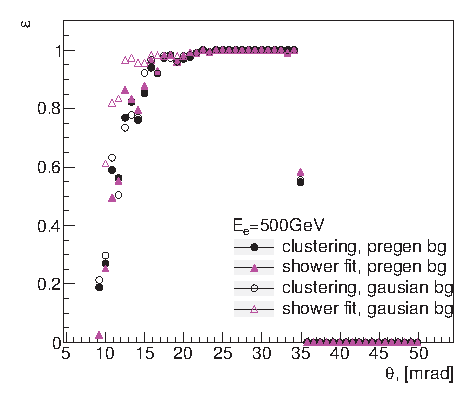
\includegraphics[width=\textwidth]{{{doubleHiggs/forward/ForwardBCAL}}}
    \caption{}
    \label{fig:doubleHiggsForwardBCAL}
  \end{subfigure}
  \hfill
  \begin{subfigure}[b]{0.45\textwidth}
    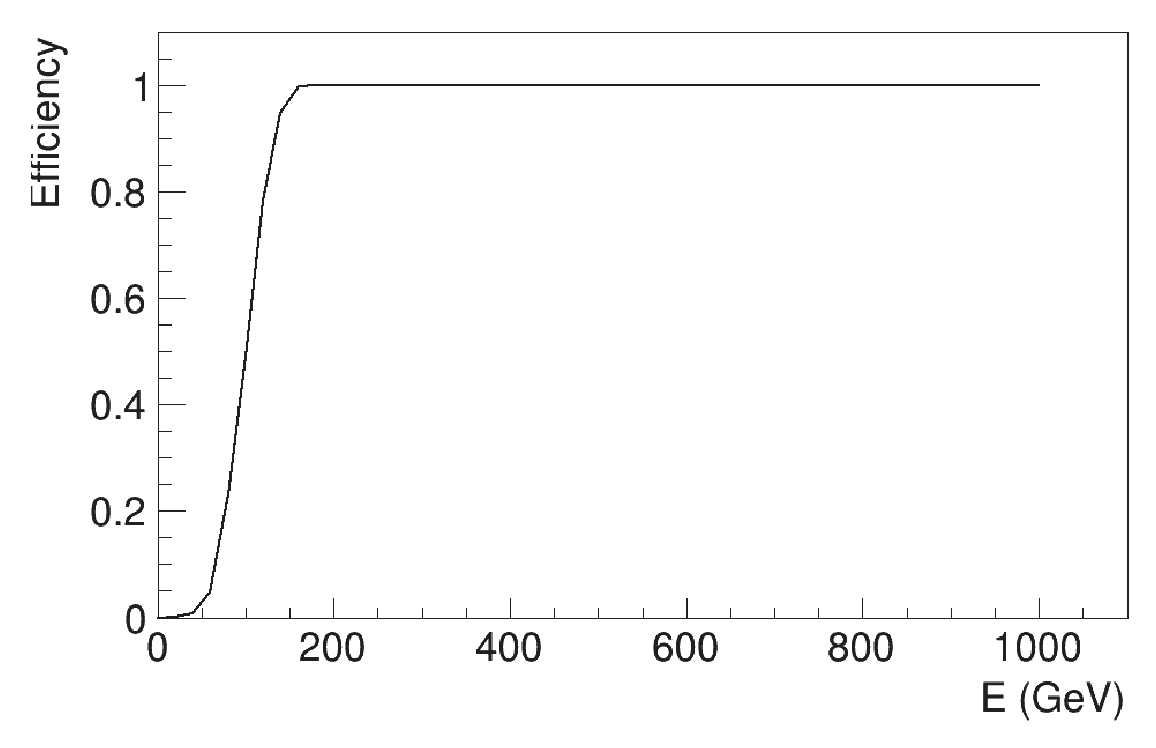
\includegraphics[width=\textwidth]{{{doubleHiggs/forward/ForwardLCAL}}}
    \caption{}
    \label{fig:doubleHiggsForwardLCAL}
  \end{subfigure}
\caption[\BeamCAL and \LumiCAL electron tagging efficiency.]%
   {\FIGURE{fig:doubleHiggsForwardBCAL} shows \BeamCAL 500\,GeV electron tagging efficiency as a function of polar angle with different methods to model backgrounds and fittings, taken from \cite{Sailer:2017onh}. \FIGURE{fig:doubleHiggsForwardLCAL} shows the \LumiCAL  electron tagging efficiency as a function of the electron energy, for polar angle $\theta = 50\,mrad$, taken from \cite{Lukic:forwardElectron}. }
   \label{fig:doubleHiggsForwardCAL}
\end{figure}

For the \LumiCAL,  \Figure{fig:doubleHiggsForwardCAL} shows the \LumiCAL  electron tagging efficiency as a function of the electron energy for polar angle $\theta = 50\,mrad$ where events are overlaid with background energy deposition integrated over 100 bunch crossings. Assuming that the \LumiCAL electron tagging efficiency in this analysis is the same as in \Figure{fig:doubleHiggsForwardCAL} for all polar angles and for \rootS{1.4} and 3\,TeV, \LumiCAL electron tagging efficiency, $\varepsilon$, is parameterised as

%The \LumiCAL electron tagging in this analysis is based on the performance plot in \Figure{fig:doubleHiggsForwardCAL}.

%the \HepProcess{\PHiggs \to \Pmu \Pmu} analysis in \cite{Milutinovic-Dumbelovic:2014uta,Grefe:2012rt} has developed an algorithm for electron tagging in the \LumiCAL with similar logic to the algorithm for the \BeamCAL.
% as this is the only study available for comparison.


\begin{equation}
\varepsilon=
\begin{cases}
  0, & \text{if}\ E < 50\,GeV,\\
  0.99 \times \frac{(erf(E - 100) + 1 )}{2}, & \text{otherwise},
\end{cases}
\end{equation}
where $E$ is the energy of the electron or the photon and $erf$ is the error function. For each MC electron in the \LumiCAL a random number between 0 and 1 is generated. If the random number is less than \varepsilon the MC electron is tagged.

%(see \Table{tab:detectorForwardILDvsCLICILD} for detector coverage)
Due to lack of tracking ability in the forward region, electrons and photons can not be differentiated in forward calorimeters. Therefore, both photons and electrons are tagged by the above algorithms.

%appear indistinguishable to the \BeamCAL and \LumiCAL and both photons and electrons are tagged by the above algorithms.


 %Due to the lack of tracking in these region, electrons and photons would have the same electromagnetic shower profile, with the given calorimeter resolution. MC photons and electrons are checked if they fall in the LCal or the BCal, and checked against the known detection efficiency.


%With the increase of the centre-of-mass energy, more  As discussed before, veto events with leptons help the signal selection. Hence the goal is to identify leptons in the forward region.

%These forward calorimeters were not simulated due to computational limitation.
% For \rootS(3), the BeamCal detection efficiency is provided by a software package \cite{}. For \rootS(1.4), the same software for the BeamCal is used, by scaling the energy of the MC particle by a factor of $\frac{3}{1.4}$. For the LumiCal, the identification efficiency is defined as


\subsection{Lepton identification performance}

The performance of all lepton finding processors on the signal and selected background process is shown in \Table{tab:doubleHiggsIsoLepPerformance}. The percentages represent the events without identified primary leptons.  \BonoLeptonFinder and \BonoTauFinder reject more background events than the \IsolatedLeptonFinderProcessor and \TauFinderProcessor. By combining the processors, 86.6\% signal events remain and 16.8\% of \HepProcess{\Pep \Pem \to \Pquark\Pquark\Pquark\Pquark\Plepton\Pnu} events survive after rejecting events where leptons are identified.
%Second sentence: can you say "" becase this would read better

\begin{table}[!tbp]
\begin{tabular}{lrr}
\hline
\hline
Efficiency (1.4\,TeV)  &  Signal & \HepProcess{\Pep \Pem \to \Pquark\Pquark\Pquark\Pquark\Plepton\Pnu} \\
\hline
\IsolatedLeptonFinderProcessor & 99.3\% & 50.3\%  \\
\BonoLeptonFinder & 99.1\% & 39.9\%  \\
\TauFinderProcessor & 97.5\% & 52.3\%  \\
\BonoTauFinder & 89.7\% & 38.5\%  \\
Forward Finder Processors & 98.9\% & 95.1\%  \\
\hline
Combined & 86.6\% & 16.8\%  \\
\hline
\hline

\end{tabular}
\caption{Isolated lepton finder processors performance on the signal and selected background events at \rootS{1.4}.}
\label{tab:doubleHiggsIsoLepPerformance}
\end{table}


The forward lepton finders are most effective at rejecting background events with primary leptons in the forward region. \TABLE{tab:doubleHiggsForwardPerformance} shows the performance of the processors with the signal and the  \egamma{\Pem}{\Pphoton}{BS}{\Pem \Pquark \Pquark \Pquark \Pquark} background events. 53.6\% of \egamma{\Pem}{\Pphoton}{BS}{\Pem \Pquark \Pquark \Pquark \Pquark} background events survive after rejecting events with primary leptons identified.


\begin{table}[!tbp]
\begin{tabular}{lrr}
\hline
\hline
Selection / Efficiency (1.4\,TeV)  &  Signal & \egamma{\Pem}{\Pphoton}{BS}{\Pem \Pquark \Pquark \Pquark \Pquark}  \\
\hline
Combined light lepton finder & 87.6\% & 67.5\%  \\
Forward Finder Processors & 98.9\% & 53.6\%  \\
\hline
Combined & 86.6\% & 30.8\%  \\
\hline
\hline

\end{tabular}
\caption{Very forward electron and photon finder performance on the signal and selected background events at \rootS{1.4}.}
\label{tab:doubleHiggsForwardPerformance}
\end{table}


\subsection{Other lepton identification processors}


Other isolated lepton identification processors have been tested, including IsolatedLeptonTagging and TauJetClustering. They either performed poorly comparing to the processors above, or became redundant after using the processors above. Therefore, these lepton identification processors are not used in this analysis.
%ATTN: does calibration/optimisation work better than tuning parameters?

\section{Jet reconstruction}

For the signal channel, \eeToHHbbWWHad, one Higgs boson decays to two \Pbottom quarks, resulting in two jets from quark hadronisation. Similarly the other Higgs boson decays to two \PW bosons, where each \PW boson decays into two quarks. Therefore, the expected number of jets is six.  Physical bosons,  \PW and \PHiggs, can be reconstructed from jets. Therefore, it is important to have efficient jet reconstruction to reconstruct physical bosons and the signal events. In this section, the optimisation of the jet reconstruction is discussed.

% A useful technique for the analysis is to reconstruct the multi-jet final state using jet algorithms. This allows discriminative variables to be calculated. A brief discussion about jet algorithms and its relevance for the \CLIC and this analysis are provided.

\subsection{Jet reconstruction optimisation}
\label{sec:doubleHiggsJetOptimisation}
Jet reconstruction algorithms group particles into jets. An overview of the jet algorithms can be found in \Section{sec:pandoraJetAlg}. Longitudinal invariant, \kt, jet algorithm is chosen for the jet clustering. The free parameters for \kt algorithm are the $R$ parameter, which controls the radius of the jet, and the choice of the \PFO collection, which incorporates different level of timing and \pT cuts to reduce beam induce background (see \Section{sec:pandoraggHad}).
%Both parameters are optimised for \rootS{1.4} and \rootS{3}.

The metric for optimising the $R$ parameter, and the \PFO collection, is the invariant mass and mass resolution of \PHiggs and \PW. An optimised jet reconstruction is chosen such that invariant masses of \PHiggs and \PW are close to their true masses, and invariant mass widths are small.

%For the jet reconstruction optimisation, only signal events are used and jets are paired to using MC truth information (see \Section{sec:pandoraMCtruthLink}).

%The sample for the optimisation is \eeToHH.

The signal channel, hadronic decay of \eeToHHbbWWHad, is used for the jet reconstruction optimisation. The signal events  are processed through \kt jet algorithm  in the 6-jet exclusive mode. The six jet are paired using the MC truth information (see \Section{sec:pandoraMCtruthLink}) by examining the decay chain of MC particles. Four invariant mass distributions are obtained: two Higgs masses, $m_{\Hbb}$, $m_{\HWW}$, and two \PW masses $m_{\PW}$, $m_{\W*}$. \W* indicates the off-mass-shell \PW boson because when a Higgs boson decays into two \PW bosons, one \PW is off the mass shell, as the Higgs mass is less than the sum two \PW masses (see \Section{sec:theoryHiggsBoson}).
%The six jets are paired up using  MC truth information to the corresponding Higgs and \PW boson.
%I'm not sure this last sentence is worded correctly. Doesn't make sense to me but I'm not a physicist!

\paragraph{Mass resolution fit}
Three invariant mass distributions are compared for optimising jet reconstruction:  $m_{\Hbb}$, $m_{\HWW}$, and $m_{\PW}$. The optimal jet reconstruction should produce a sharp mass peak around the particle's simulated mass (see \Section{sec:pandoraCLICsimMass}). An example of $m_{\Hbb}$ invariant mass distribution is shown in \Figure{fig:doubleHiggsFitMCMass}. An analytical functional form is fitted to quantitatively describe the shape. The basic fitting function is a Gaussian function. Although the underlying mass distribution of particles like $m_{\PW}$ is a Breit-Wigner distribution, the overall mass distribution is Gaussian like, as the overall mass distribution is a convolution of a narrow \PW Breit-Wigner distribution and a wide Gaussian distribution for the detector resolution. The $m_{\Hbb}$  mass distribution is gaussian like but with asymmetrical width, due to \Pbottom quarks decaying to neutrinos, leading to a loss of detectable particles.

As only the peak region of the mass distribution is Gaussian like, free parameters are used in the fitting function to fit the tail distribution. The fitting function takes the form of
\begin{equation}
f(m)=A e^{- \frac{(m - \mu)^2}{g}}
\end{equation}
\begin{equation}
g=
\begin{cases}
2\sigma_L + \alpha_L(m - \mu), & \text{if}\ m < \mu,\\
2\sigma_R + \alpha_R(m - \mu), & \text{if}\ m \geqslant \mu,
\end{cases}
\end{equation}
where $m$ is binned mass distribution with 50 bins in range [0, 200]\,GeV. $\mu$ is the fitted mass peak position in GeV. $\sigma_L$ and $\sigma_R$ allow asymmetrical width of the distribution. $\alpha_L$ and  $\alpha_R$  control the fit of tail distribution.  $A$ is the normalisation factor.


\begin{figure}[!htbp]
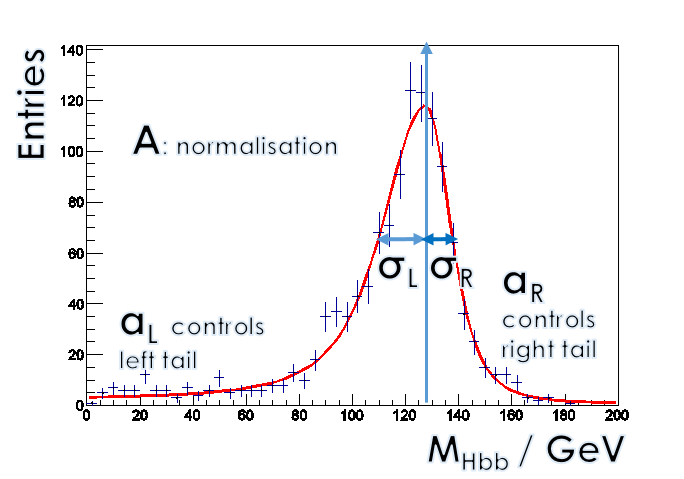
\includegraphics[width=\largefigwidth]{doubleHiggs/MCmassFit}
\caption[Example MC mass fit for jet optimisation in double Higgs analysis]%
   {A typical example of  $m_{\Hbb}$  mass distribution with the superimposed fitting function in red. The arrow shows the fitted mean peak position in GeV.}
   \label{fig:doubleHiggsFitMCMass}
\end{figure}

\paragraph{Optimal $R$ and \PFO collection}

%The mass fit is performed for $m_{\Hbb}$, $m_{\HWW}$, and $m_{\PW}$ distributions.  The optimal jet reconstruction should have the mass peak close to the particle's simulated mass and a narrow peak width.

Due to the asymmetrical functional fit, the overall relative width is defined as $\left(\sigma_L  + \sigma_R\right)/M$. Smaller width indicates better mass resolution. This mass fit is repeated for reconstruction with $R$ values of 0.5 to 1.3, at interval of 0.1, and with three \PFO collections: loose, normal, and tight (see \Section{sec:pandoraggHad}).

\FIGURE{fig:doubleHiggs1.4TeVMassFit} shows the mass peak and the relative width as a function of $R$ and \PFO collections, for $m_{\Hbb}$, $m_{\HWW}$, and $m_{\PW}$. The mass peak position, $\mu$, increases as $R$ increases. This is because more particles are included in jets with increasing jet radius. Hence a larger invariant mass is obtained. For the relative width, the values for \Hbb in \Figure{fig:doubleHiggs1.4Higgs1Sigma} increase with increasing jet radius, but the values for \HWW  in \Figure{fig:doubleHiggs1.4Higgs2Sigma} decrease  with increasing jet radius. This is due to a compensating effect. \HWW decays to 4 jets, which prefers a large jet radius, whilst \Hbb decays to 2 jets, which prefers a small jet radius. Similarly, \PW prefers a small jet radius and the relative width increases with increasing $R$.

The choice of \PFO collection impacts number of \PFOs in the event. The loose \PFO selection has the most \PFOs in the event and, therefore, the largest invariant mass and worst mass resolution. This trend is consistent when comparing three \PFO collections.

The optimal choice, \normalPFO with $R = 0.7$  gives good fitted mass peak positions for \Hbb, \HWW and \PW. The extracted fitted parameters of optimal jet reconstructions are summarised in \Table{tab:doubleHiggsFitParameters}.


\begin{figure}[!tbp]
  \begin{subfigure}[b]{0.45\textwidth}
    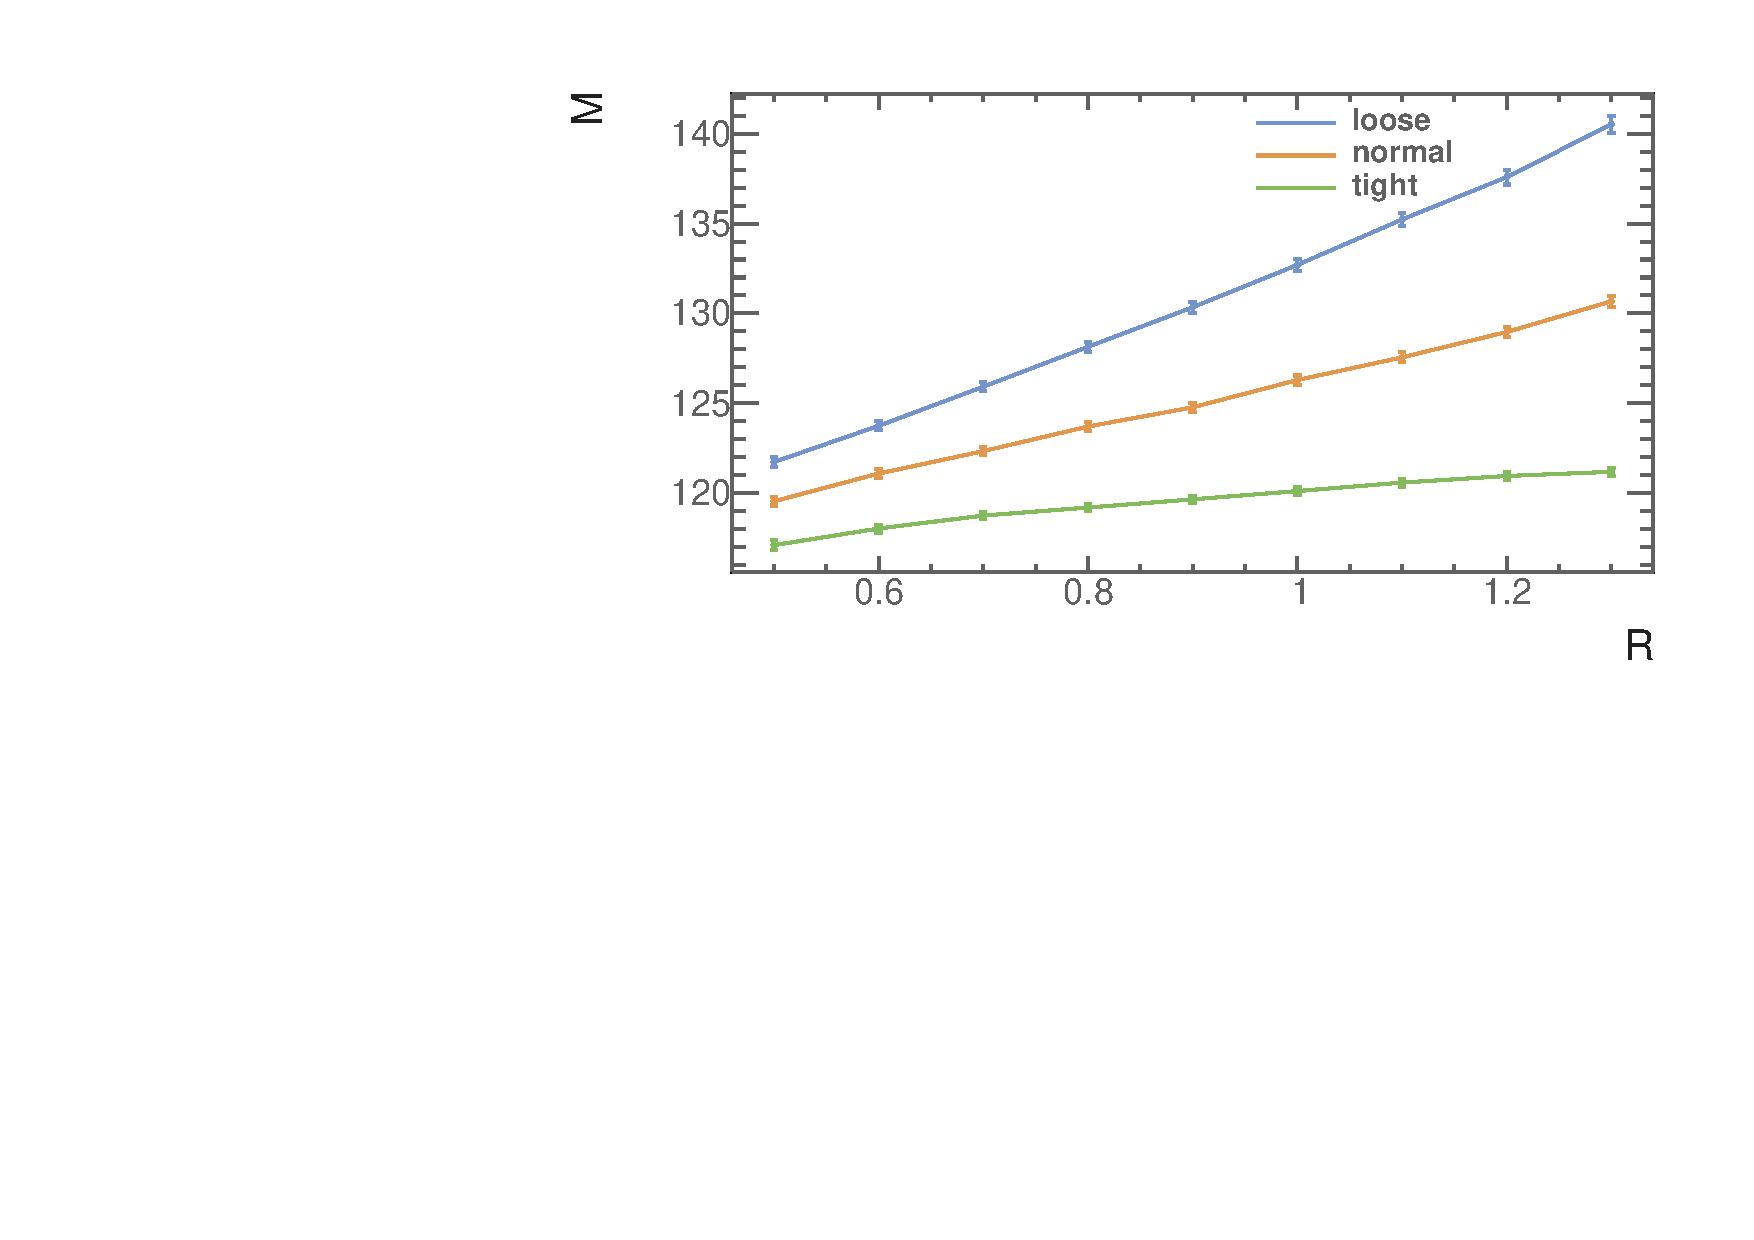
\includegraphics[width=\textwidth]{{doubleHiggs/resolution/ILD_1.4TeV_Higgs1_M_R}.pdf}
    \caption{}
    \label{fig:doubleHiggs1.4Higgs1M}
  \end{subfigure}
  \begin{subfigure}[b]{0.45\textwidth}
    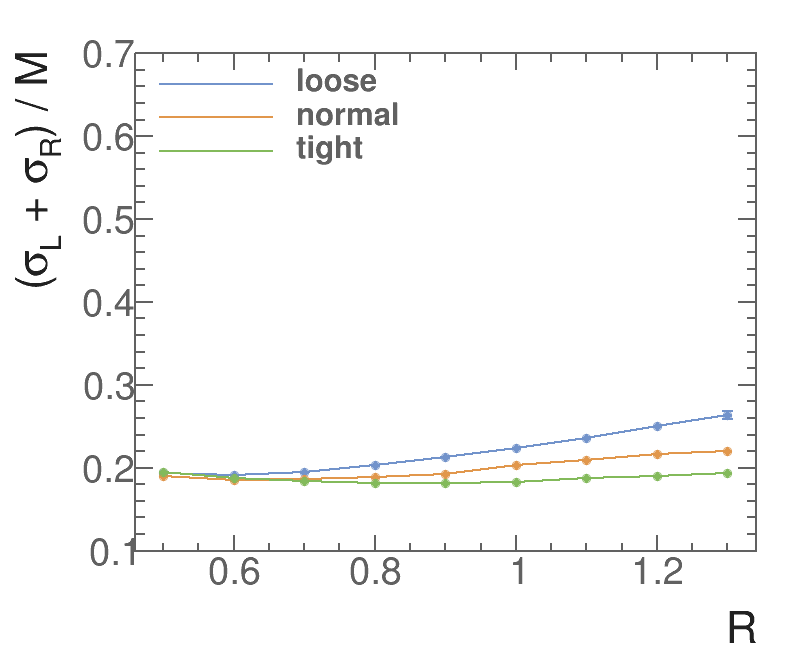
\includegraphics[width=\textwidth]{{doubleHiggs/resolution/ILD_1.4TeV_Higgs1_SigmaL_add_SigmaR_divide_M_testR}.pdf}
    \caption{}
    \label{fig:doubleHiggs1.4Higgs1Sigma}
  \end{subfigure}
  \begin{subfigure}[b]{0.45\textwidth}
    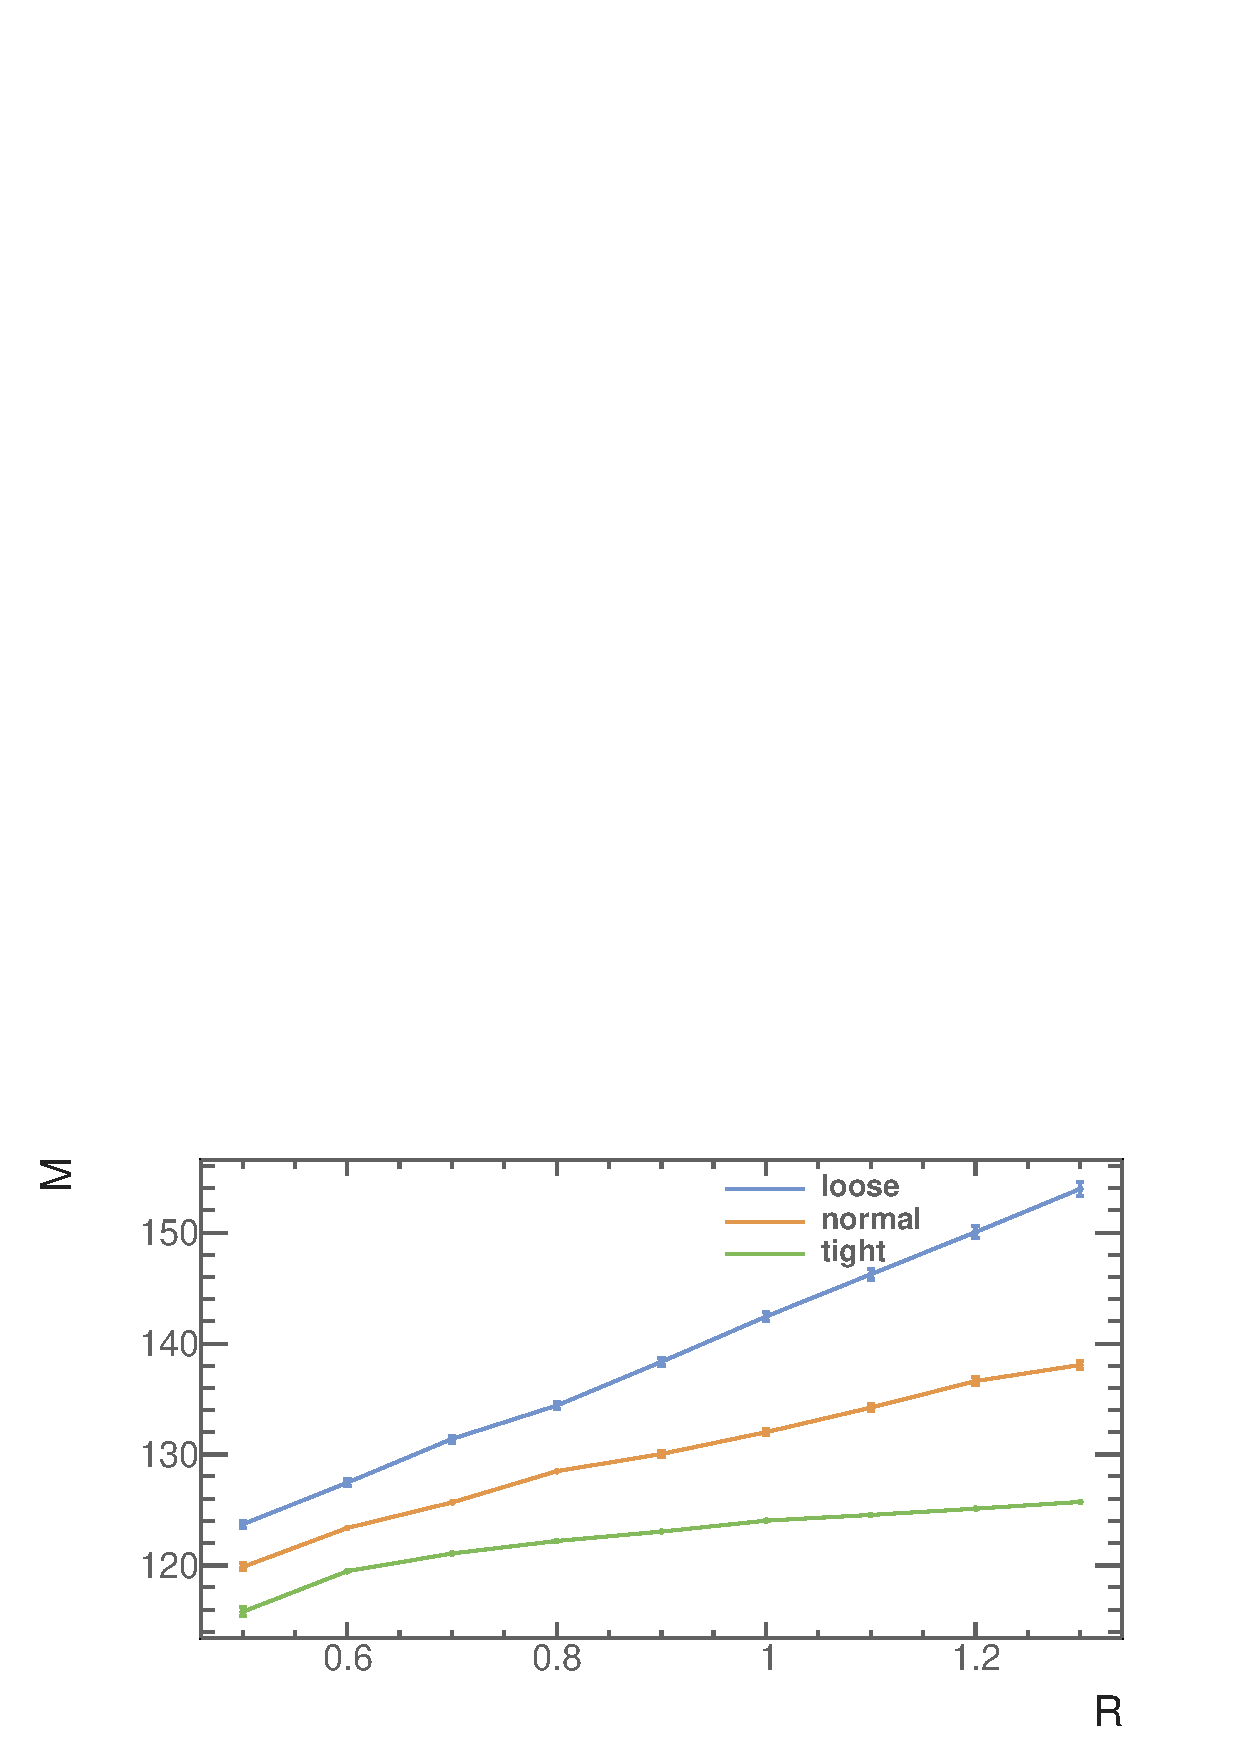
\includegraphics[width=\textwidth]{{doubleHiggs/resolution/ILD_1.4TeV_Higgs2_M_R}.pdf}
    \caption{}
    \label{fig:doubleHiggs1.4Higgs2M}
  \end{subfigure}
  \begin{subfigure}[b]{0.45\textwidth}
    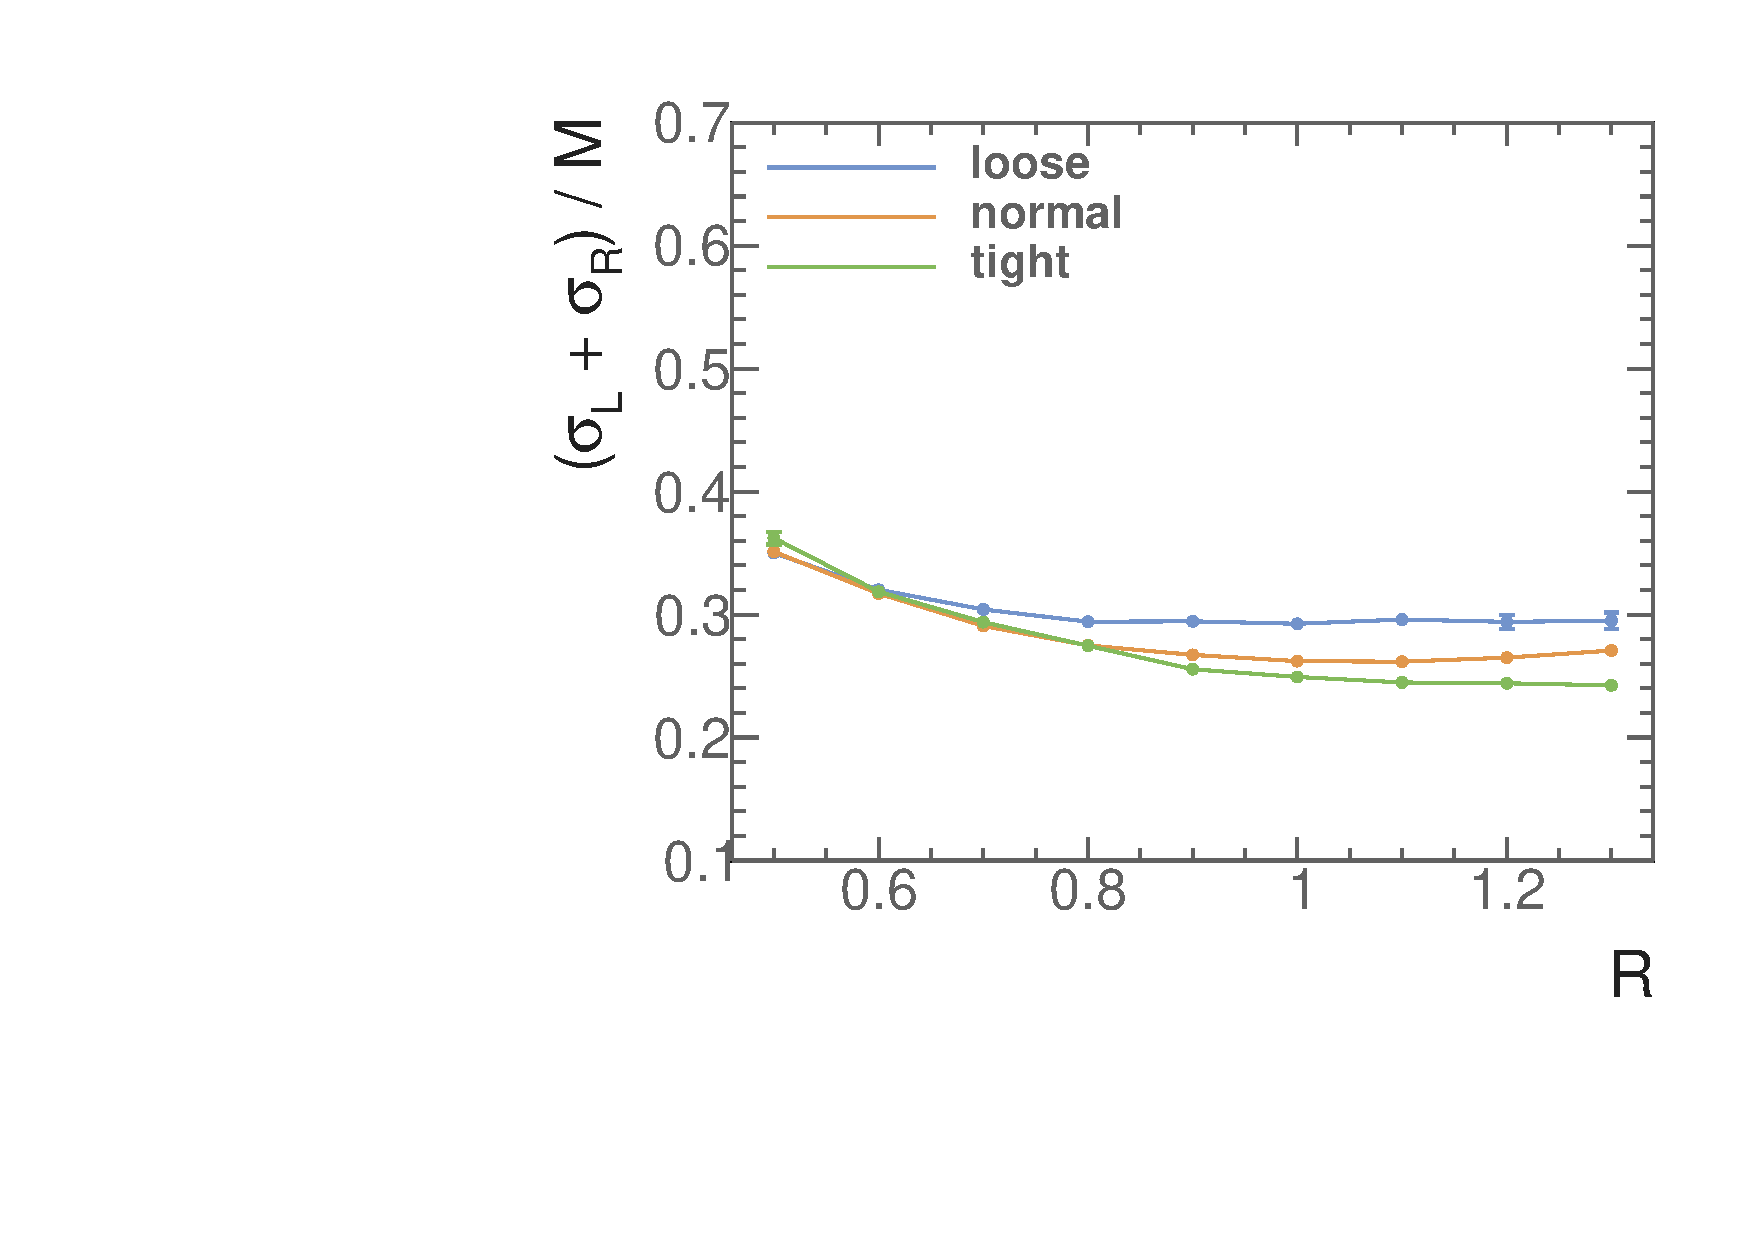
\includegraphics[width=\textwidth]{{doubleHiggs/resolution/ILD_1.4TeV_Higgs2_SigmaL_add_SigmaR_divide_M_testR}.pdf}
    \caption{}
    \label{fig:doubleHiggs1.4Higgs2Sigma}
  \end{subfigure}
  \begin{subfigure}[b]{0.45\textwidth}
    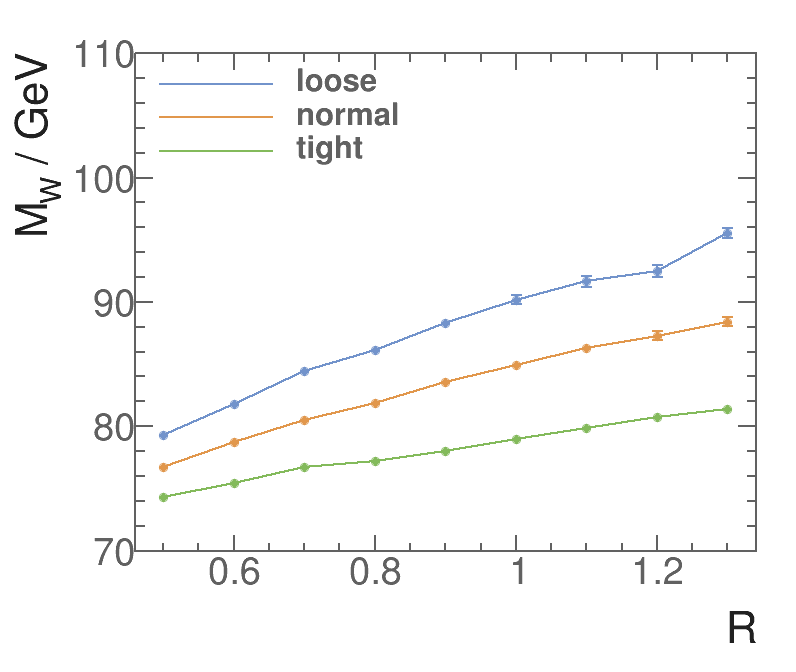
\includegraphics[width=\textwidth]{{doubleHiggs/resolution/ILD_1.4TeV_W_M_testR}.pdf}
    \caption{}
    \label{fig:doubleHiggs1.4WM}
  \end{subfigure}
  \begin{subfigure}[b]{0.45\textwidth}
    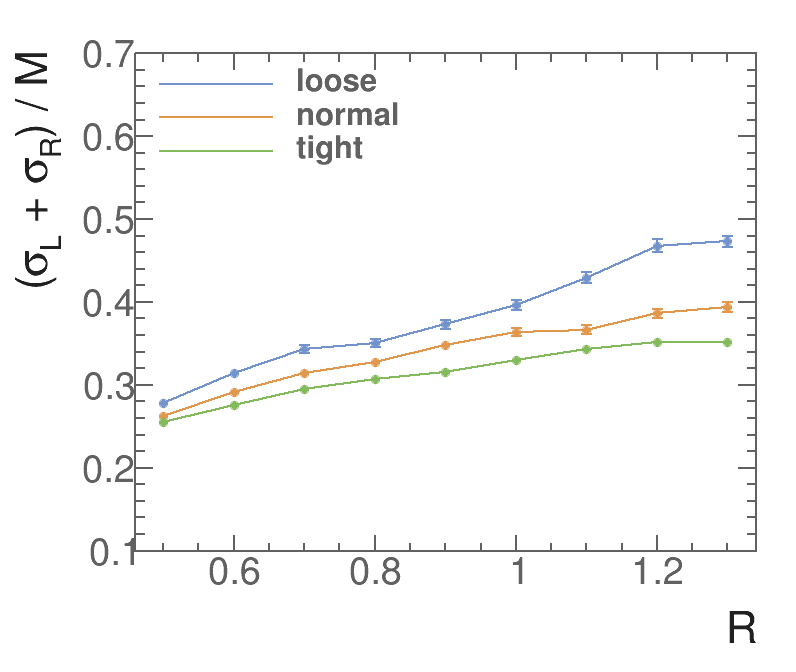
\includegraphics[width=\textwidth]{{doubleHiggs/resolution/ILD_1.4TeV_W_SigmaL_add_SigmaR_divide_M_testR}.pdf}
    \caption{}
    \label{fig:doubleHiggs1.4WSigma}
  \end{subfigure}
\caption[Fitted mass, and resolution of \Hbb, \HWW and \PW at \rootS{1.4}]%
   {\FIGURE{fig:doubleHiggs1.4Higgs1M}, \ref{fig:doubleHiggs1.4Higgs2M}, and \ref{fig:doubleHiggs1.4WM}  show fitted mass peak positions of \Hbb, \HWW, and \PW as a function of $R$, for loose, normal and tight selected PFO collection at \rootS{1.4}. \FIGURE{fig:doubleHiggs1.4Higgs1Sigma}, \ref{fig:doubleHiggs1.4Higgs2Sigma}, and \ref{fig:doubleHiggs1.4WSigma} show relative mass peak width of \Hbb, \HWW, and \PW as a function of $R$  for loose, normal and tight selected \PFO collection at \rootS{1.4}.}
   \label{fig:doubleHiggs1.4TeVMassFit}
\end{figure}

\begin{table}[!htbp]
\begin{tabular}{lr}
\hline
\hline
Fitted jet parameters  &  \rootS{1.4}  \\
\hline
$\mu_{\Hbb}$ & $122.3_{\pm0.2}$  \\
$\sigma_{L,\Hbb}$ & $15.2_{\pm0.2}$   \\
$\sigma_{R,\Hbb}$ & $7.55_{\pm0.16}$   \\
\hline
$\mu_{\HWW}$ & $125.7_{\pm0.2}$   \\
$\sigma_{L,\HWW}$ & $29.4_{\pm0.3}$  \\
$\sigma_{R,\HWW}$ & $7.18_{\pm0.17}$ \\
\hline
$\mu_{\PW}$ & $80.5_{\pm0.2}$\\
$\sigma_{L,\PW}$ & $16.2_{\pm0.3}$  \\
$\sigma_{R,\PW}$ & $9.03_{\pm0.16}$  \\
\hline
\hline
\end{tabular}
\caption
[The fitted parameters of optimal jet reconstruction at \rootS{1.4}] %
{The fitted parameters of optimal jet reconstruction, \normalPFO with $R = 0.7$, at \rootS{1.4}.}
\label{tab:doubleHiggsFitParameters}
\end{table}

\section{Jet flavour tagging}
\label{sec:doubleHiggsFlavourTagging}

As the signal channel, \eeToHHbbWWHad,  has two \Pbottom quarks in the final state, identifying jets originated from \Pbottom quarks help to select signal events. To establish the likelihood of a \Pbottom jet, also known as \Pbottom tag value, \lcfiplus \cite{Suehara:2015ura} software package is used. An overview of the flavour tagging processor is provided in \Section{sec:pandoraLCFI}.

The flavour tagging is performed after the initial jet reconstruction using optimal jet reconstruction parameters.  \PFOs in the reconstructed jets are the inputs to the flavour tagging processor. \lcfiplus processor includes a multiclass classifier which needs to be trained. The samples for training the multiclass classifier are \HepProcess{\Pep \Pem \to \PZ \APnu \Pnu} at \rootS{1.4}, where \PZ decays to \HepProcess{\Pbottom\APbottom}, \HepProcess{\Pcharm\APcharm}, or \HepProcess{\Pup\APup/\Pdown\APdown/\Pstrange\APstrange}. At the training stage, the  jet clustering step is set to find two jets. The outputs for a jet is three values, corresponding to the likelihood of the jet being a b-jet, a c-jet, or a light flavour quark jet.  The selection efficiency of b jets and c jets with training samples is shown in \Figure{fig:doubleHiggs1.4Btag}.


\begin{figure}[!tbp]
    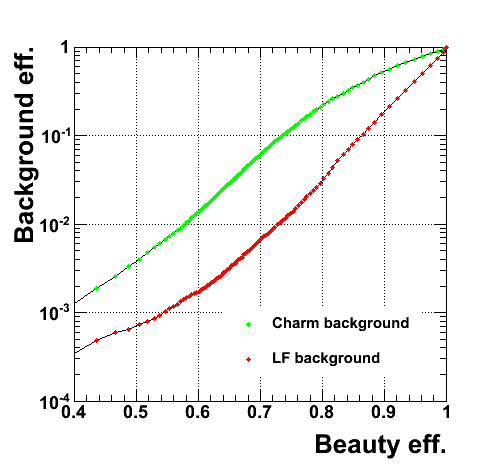
\includegraphics[width=0.45\textwidth]{{doubleHiggs/eval-lcfiweights_R0_7_2jets-test}.pdf}
    \caption
   {Performance of b-jet tagging with training samples at \rootS{1.4}.}
   \label{fig:doubleHiggs1.4Btag}
\end{figure}

To use the trained  multiclass classifier in the \lcfiplus processor, all the \PFOs in the initial reconstructed jet are fed into the processor. The jet clustering step in the \lcfiplus is set to find six jets. For each jet, values for the likelihood of a b-jet and a c-jet are obtained.

\section{Jet pairing}

Having optimised the jet reconstruction, and obtained the six jets from the jet clustering step in the \lcfiplus processor, the next step is to group jets according to event topology. Jets are paired up such that there are two jets for \HepProcess{\PHiggs \to \Pbottom \APbottom}, two jets for hadroinc decay of a \PW, two jets  for hadroinc decay  of a \W*, and the two $\PW{s}$ forming a  \PHiggs boson.
%off-mass-shell and off the mass shell? Is the "the" pertinent? Should they both be hyphenated?

The jet pairing scheme provides reconstructed invariant masses of \Hbb, \HWW, and \PW. The jet pairing metric states:
\begin{equation}
	\chi^2 = \left(\frac{m_{ij}-\mu_{\Hbb}}{\sigma_{\Hbb}^{\prime}}\right)^2 + \left(\frac{m_{klmn}-\mu_{\HWW}}{\sigma_{\HWW}^{\prime}}\right)^2  + \left(\frac{m_{kl}-\mu_{\PW}}{\sigma_{\PW}^{\prime}}\right)^2,
%\label{eqn:eq_chi2_HHWWbb}
\end{equation}

\begin{equation}
	\sigma_{\Hbb}^{\prime}=
    \begin{cases}
      \sigma_{L,\Hbb}, & \text{if}\ m_{ij} < \mu_{\Hbb}\\
     \sigma_{R,\Hbb}, & \text{otherwise} \\
   \end{cases}
\end{equation}

\begin{equation}
	\sigma_{\HWW}^{\prime}=
    \begin{cases}
      \sigma_{L,\HWW}, & \text{if}\ m_{klmn} < \mu_{\HWW}\\
     \sigma_{R,\HWW}, & \text{otherwise} \\
   \end{cases}
\end{equation}


\begin{equation}
	\sigma_{\PW}^{\prime}=
    \begin{cases}
      \sigma_{L,\PW}, & \text{if}\ m_{kl} < \mu_{\PW}\\
     \sigma_{R,\PW}, & \text{otherwise} \\
   \end{cases}
\end{equation}

where $i$ to $l$ indicate the one of the six jets with all possible combinations. $\mu$ and $\sigma$ are the fitted invariant mass and the fitted width from \Table{tab:doubleHiggsFitParameters}. The asymmetrical structure of the fitting function is reflected in the jet pairing metric. The paired jets with minimal $\chi^2$ is chosen with an additional requirement of at least one of two jets forming \Hbb having a \Pbottom-jet tag greater than 0.2.


\section{Pre-selection}
\label{sec:doubleHiggsPreSelection}
With reconstructed jets paired up, kinematic and topological variables can be calculated for the signal selection. A set of pre-selection cuts are placed to aid the multivariate analysis. The pre-selection cuts have three categories: discriminative pre-selection cuts, the mutually exclusive cuts with the \eeToHHbbqqqq sub-channel, and cuts to aid the MVA.

\subsection{Discriminative pre-selection cuts}

This set of  pre-selection cuts are designed to discard events that are dominated by background events. For the signal events, the double Higgs system have substantial invariant mass as both \PHiggs are on mass shell. The two \Pbottom jets in the signal final state are a clear signature. There is missing momentum as the final state contains neutrinos. The pre-selection cuts are listed in \Table{tab:doubleHiggsPreSel}. The distributions of variables used for discriminative pre-selection cuts are shown in \Figure{fig:doubleHiggs1.4TeVPreSelection}.

\FIGURE{fig:doubleHiggs1.4PreSelmHH} shows the distribution of the invariant mass of the two Higgs system, where the cut above 150\,GeV is effective against samples with two quark final states. \FIGURE{fig:doubleHiggs1.4PreSelbtag} shows the distribution of the second highest b-jet tag value, where the cut above 0.2 helps to reduce background events with no b-jets in final states. \FIGURE{fig:doubleHiggs1.4PreSelpT} shows the distribution of the transverse momentum  of the two Higgs system, where the cut above 30\,GeV  is extremely effective against background channels with no neutrinos in the final state.

\begin{table}[!htbp]
\begin{tabular}{lr}
\hline
\hline
Pre-selection  &  \rootS{1.4}  \\
\hline
Discriminative pre-selection & \multicolumn{1}{R{0.5\textwidth}}{$m_{\HH} > 150\,GeV$, $B_2 > 0.2$,  $\pT_{\HH} > 30\,GeV$} \\
Loose cuts for MVA &  \multicolumn{1}{R{0.5\textwidth}}{$m_{\Hbb} < 500\,GeV$, $m_{\HWW} < 800\,GeV$, $m_{\PW} < 200\,GeV$, $m_{\HH} < 1400\,GeV$} \\
Mutually exclusive & \sumBtag{4} < 2.3, \y{34} < 3.7 \\
\hline
\hline
\end{tabular}
\caption
{Pre-selection cuts at \rootS{1.4}.}
\label{tab:doubleHiggsPreSel}
\end{table}

\begin{figure}[!tbp]
  \begin{subfigure}[b]{0.45\textwidth}
    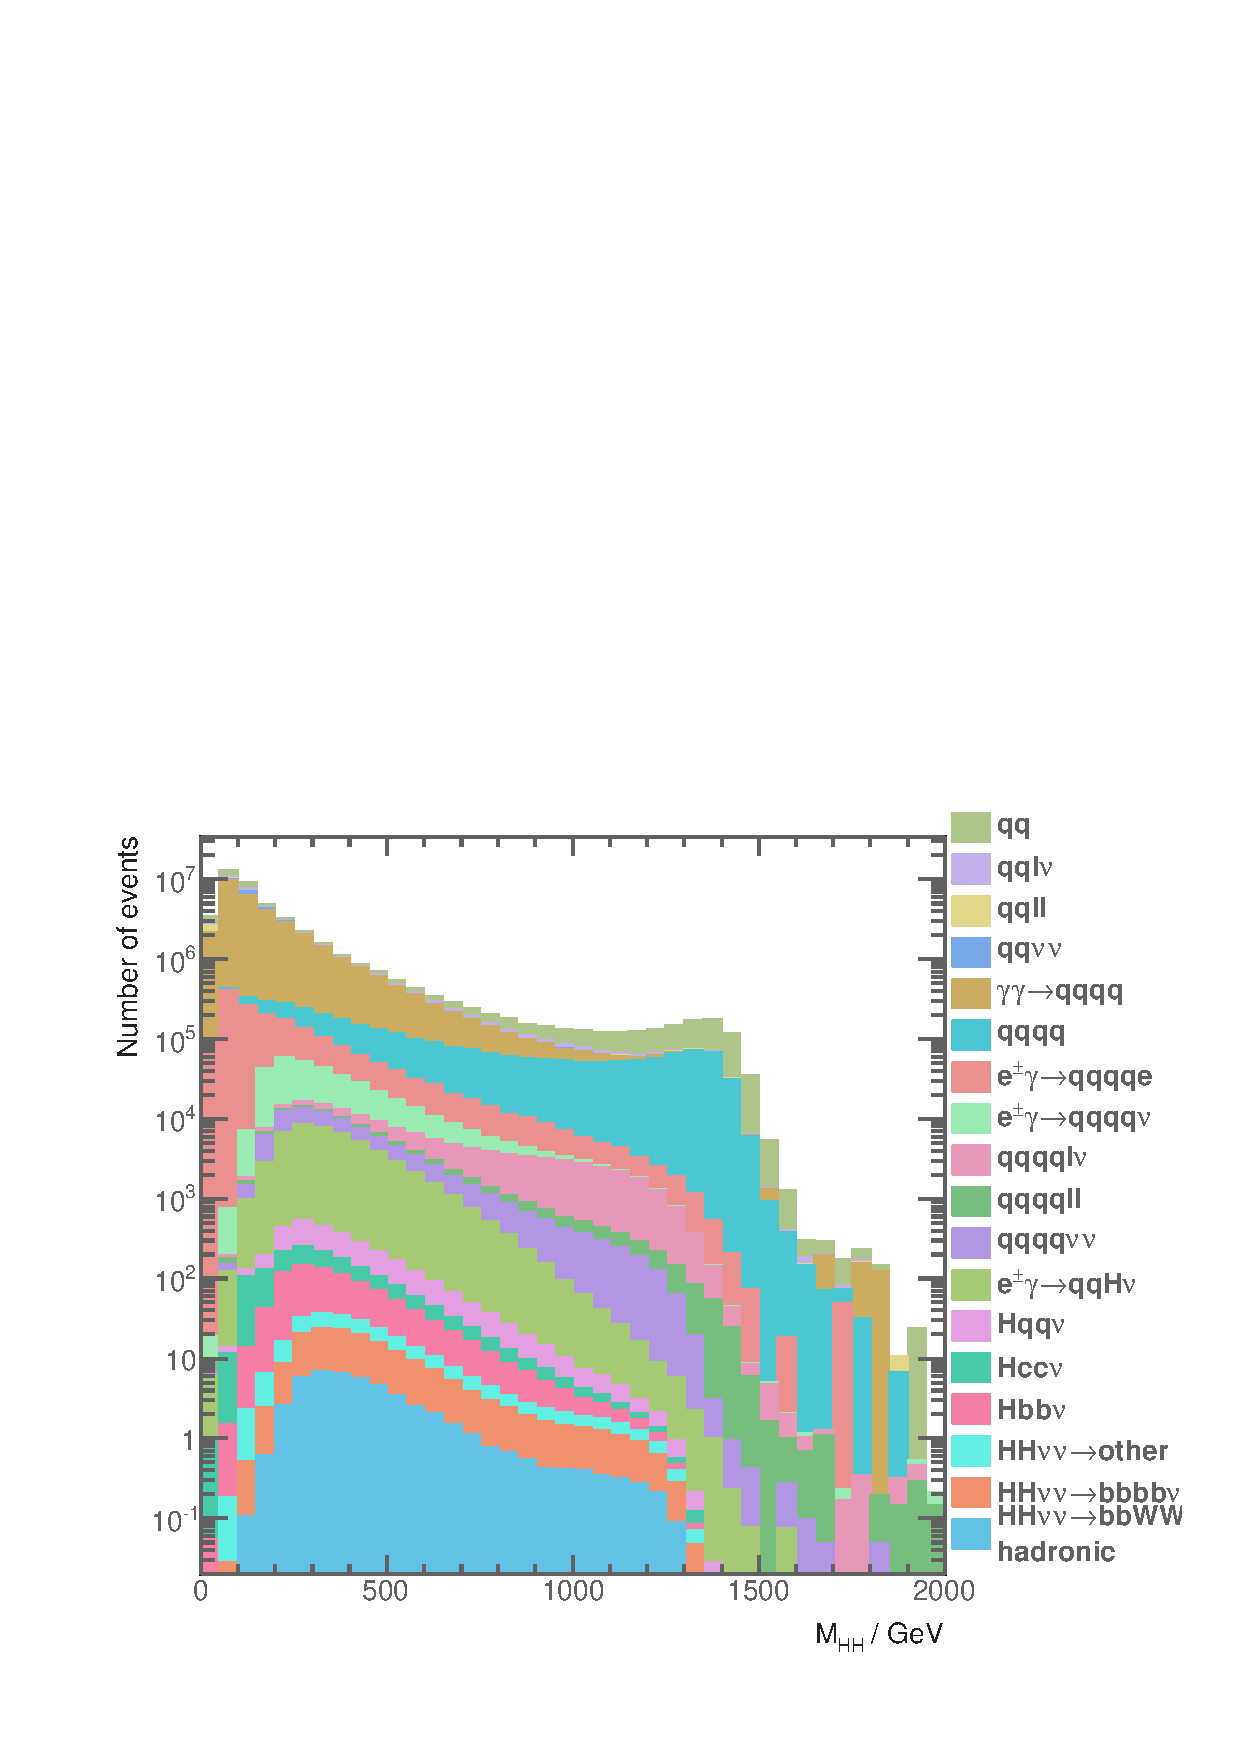
\includegraphics[width=\textwidth]{{doubleHiggs/preSel/nR0_7_6jet_btag2_Higgs_all_M_TMVA20161208R0_7_qq_btag2_prepare}.pdf}
    \caption{}
    \label{fig:doubleHiggs1.4PreSelmHH}
  \end{subfigure}
    \begin{subfigure}[b]{0.45\textwidth}
    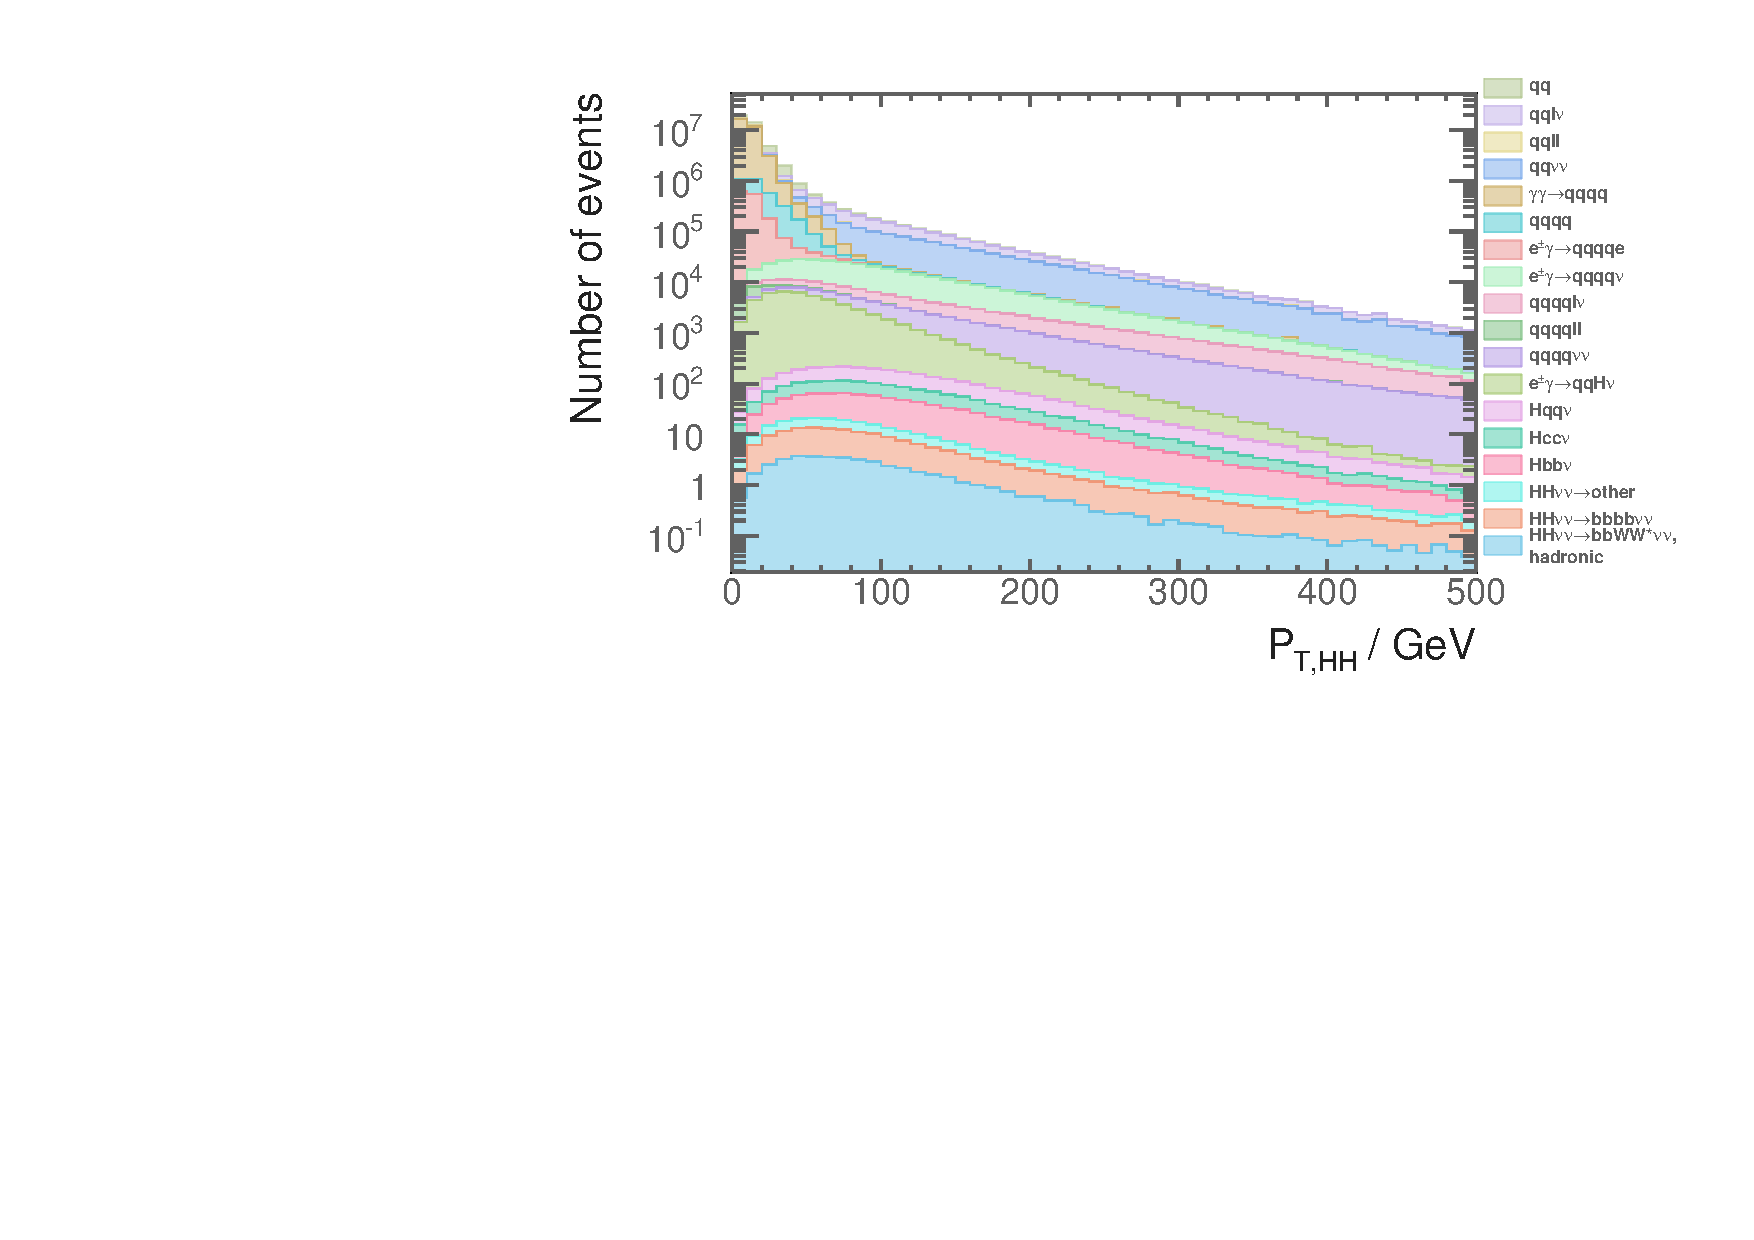
\includegraphics[width=\textwidth]{{doubleHiggs/preSel/nR0_7_6jet_btag2_Higgs_all_Pt_TMVA20161208R0_7_qq_btag2_prepare}.pdf}
    \caption{}
    \label{fig:doubleHiggs1.4PreSelpT}
  \end{subfigure}
      \begin{subfigure}[b]{0.45\textwidth}
    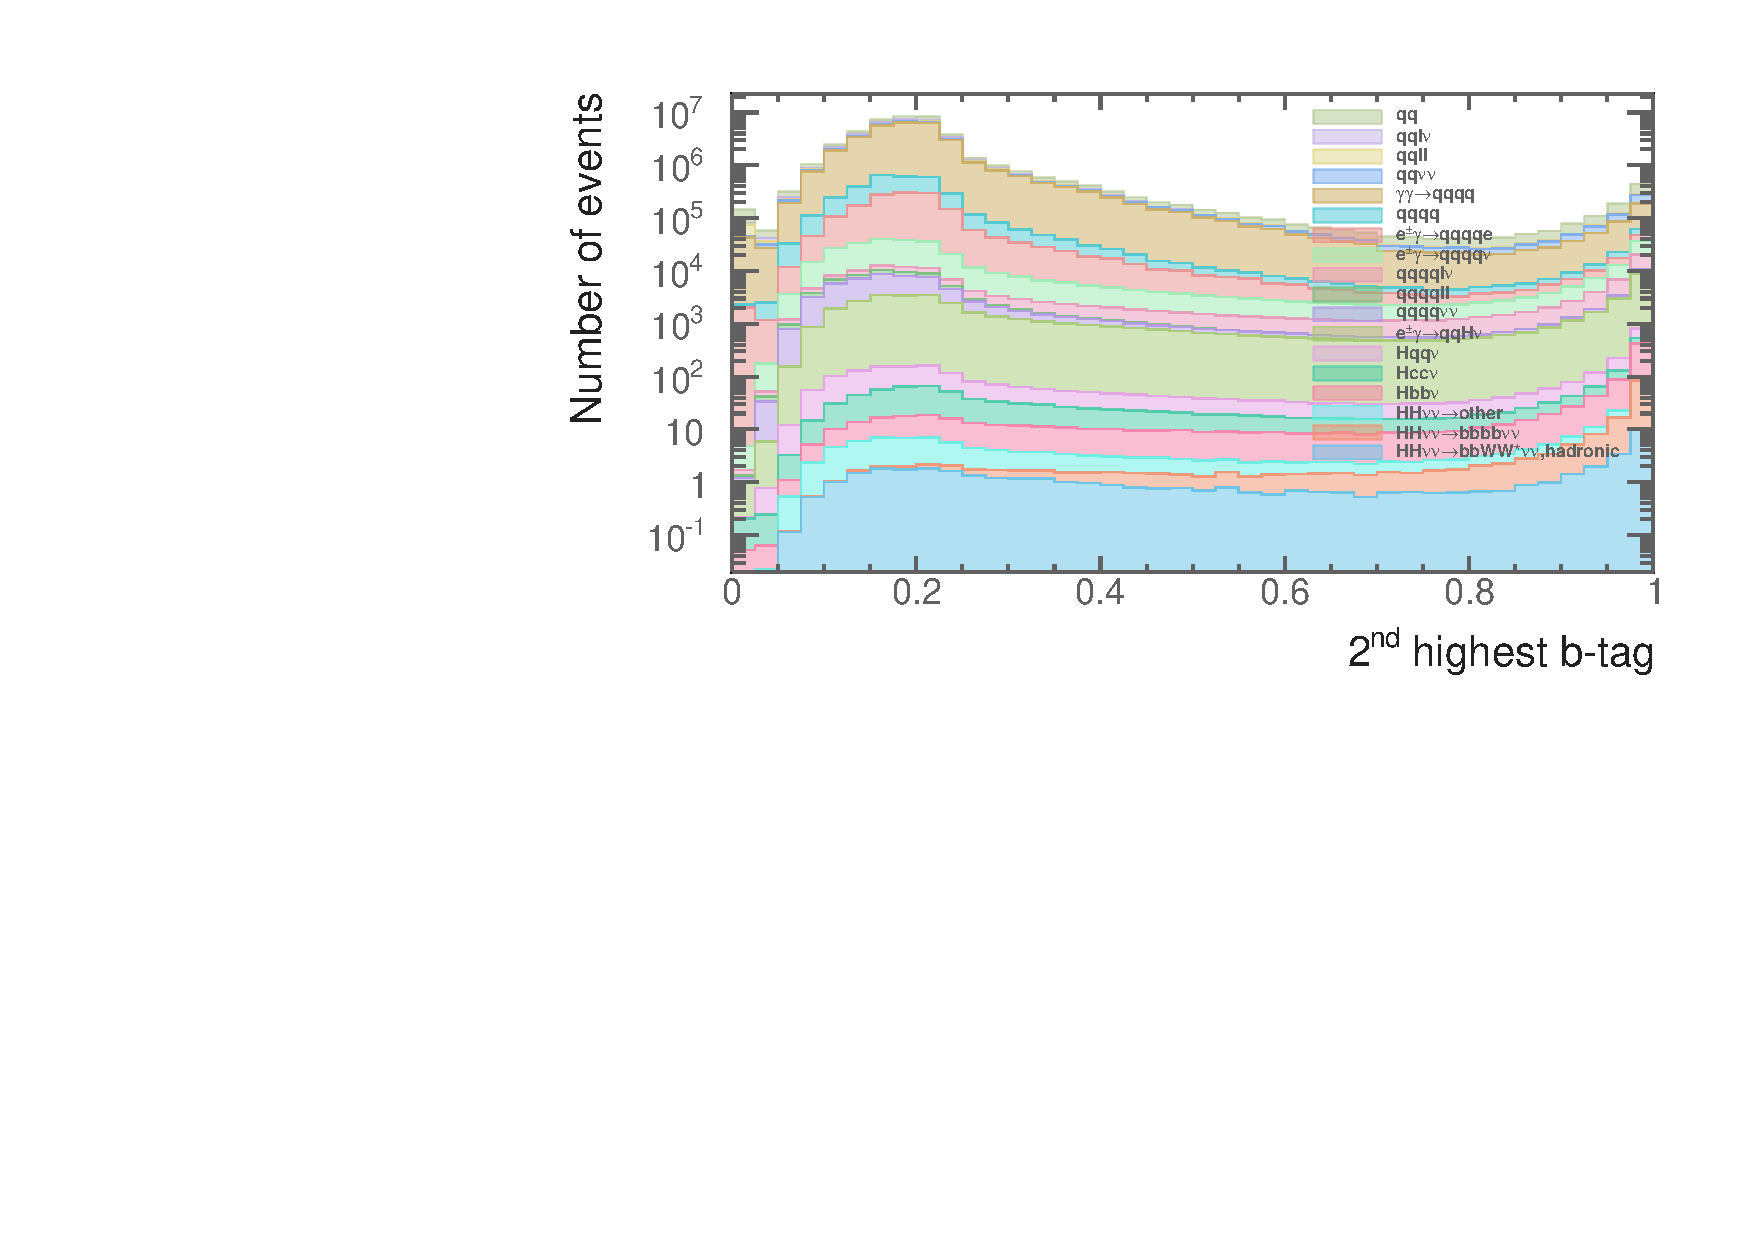
\includegraphics[width=\textwidth]{{doubleHiggs/preSel/nR0_7_6jet_btag2_bTag2_TMVA20161208R0_7_qq_btag2_prepare}.pdf}
    \caption{}
    \label{fig:doubleHiggs1.4PreSelbtag}
  \end{subfigure}

\caption[Distributions of discriminative pre-selection variables for \rootS{1.4}.]%
   {Distributions of discriminative pre-selection variables for \rootS{1.4}. \Figure{fig:doubleHiggs1.4PreSelmHH},  \Figure{fig:doubleHiggs1.4PreSelpT}, and ,  \Figure{fig:doubleHiggs1.4PreSelbtag} show distributions for he invariant mass of the two Higgs system,  the second highest b-jet tag value, and the transverse momentum  of the two Higgs system respectively.}
   \label{fig:doubleHiggs1.4TeVPreSelection}
\end{figure}


\begin{table}[!tbp]\centering
% TODO fix lumi correction for e gamma, gamma e
% TODO change some of sample cross section for  electron-photon interaction with four quarks and a neutrino final state
%\small{
\small
\begin{tabular}{lrrrrr}
\hline \hline
 \multicolumn{1}{m{3.5cm}}{Channel / Efficiency \rootS{1.4}} &  \multicolumn{1}{m{2cm}}{Expected number of events}  & \multicolumn{1}{m{2cm}}{Lepton ID and jet pairing} & \multicolumn{1}{m{1.5cm}}{$m_{HH}>150\xspace{GeV}$} & \multicolumn{1}{m{1.5cm}}{$B_{2}>0.2$} & \multicolumn{1}{m{1.5cm}}{$\Pt>30\xspace{GeV}$}  \\
\hline
\eeToHH $\to$ \\
\HepProcess{ \Pbottom \APbottom \PWplus \PWminus \Pnue \APnue}, hadronic             &27.9& 85.8\% & 85.6\% & 73.7\%& 66.4\%\\
\hline
\eeToHH $\to$ \\
\HepProcess{ \Pbottom \APbottom \Pbottom \APbottom \Pnue \APnue}             &67.6& 90.8\% & 90.5\% & 90.1\% & 80.6\%\\
\eeToHH $\to$ other & 128.0 & 36.2\% & 35.3\% & 27.7\% & 24.7\%\\
\hline
\eeTo{\qlight \qlight \PHiggs \Pnu \APnu}  & 1304.0 & 60.7\% & 59.8\% & 44.9\%& 42.0\%\\
\eeTo{\Pcharm \APcharm \PHiggs \Pnu \APnu}  & 546.1 & 67.4\%& 57.7\%& 46.5\%& 43.4\%\\
\eeTo{\Pbottom \APbottom \PHiggs \Pnu \APnu}  & 463.0 & 73.9\%& 72.6\%& 68.7\%& 64.2\%\\

\eeTo{ \Pquark \Pquark \Pquark \Pquark}   &   1867650.0& 48.8\% & 46.1\%& 17.3\%& 4.7\%\\
\eeTo{ \Pquark \Pquark \Pquark \Pquark \Plepton \Plepton}& 93150.0 & 5.0\%& 4.9\%& 1.5\%& 0.3\%\\
\eeTo{ \Pquark \Pquark \Pquark \Pquark \Plepton \Pnu}& 165600.0 & 15.1\%& 15.1\%& 12.4\%& 11.4\%\\
\eeTo{ \Pquark \Pquark \Pquark \Pquark \Pnu \APnu} & 34800.0& 50.7\%& 50.0\%& 20.1\%& 18.8\%\\

\eeTo{ \Pquark \Pquark} &  6014250.0 & 54.5\%& 17.5\%& 8.4\%& 2.2\%\\
\eeTo{ \Pquark \Pquark \Plepton \Pnu} &  6464550.0 & 14.1\%& 5.3\%& 2.0\%& 1.6\%\\
\eeTo{ \Pquark \Pquark \Pl \Pl} &  4088700.0 & 13.0\%& 1.1\%& 0.6\%& 0.1\%\\
\eeTo{ \Pquark \Pquark \Pnu \Pnu} & 1181550.0 & 60.1\%& 12.3\%& 6.2\%& 5.8\% \\
\hline
\egamma{\Pepm}{\Pphoton}{BS}{\Pepm \Pquark \Pquark \Pquark \Pquark} & 2606625.5  & 23.3\%& 10.6\%& 4.4\%& 0.4\%\\
%\egamma{\Pem}{\Pphoton}{BS}{\Pem \Pquark \Pquark \Pquark \Pquark} & 1305787.5  & 23.3\%& 10.6\%& 4.4\%& 0.4\%\\
%\egamma{\Pep}{\Pphoton}{BS}{\Pep \Pquark \Pquark \Pquark \Pquark} & 1300837.5 & 23.4\%& 10.5\%& 4.3\%& 0.4\%\\
\egamma{\Pepm}{\Pphoton}{EPA}{\Pepm \Pquark \Pquark \Pquark \Pquark} & 861000.0 & 11.1\%& 5.4\%& 2.2\%& 0.3\%\\
%\egamma{\Pem}{\Pphoton}{EPA}{\Pem \Pquark \Pquark \Pquark \Pquark} & 430650.0 & 11.1\%& 5.4\%& 2.2\%& 0.3\%\\
%\egamma{\Pep}{\Pphoton}{EPA}{\Pep \Pquark \Pquark \Pquark \Pquark}  & 430350.0 & 11.1\% & 5.3\%& 2.1\%& 0.3\%\\
\egamma{\Pepm}{\Pphoton}{BS}{\Pnu \Pquark \Pquark \Pquark \Pquark}& 178987.5  & 58.0\%& 56.5\%& 30.7\%& 27.5\%\\
%\egamma{\Pem}{\Pphoton}{BS}{\Pnu \Pquark \Pquark \Pquark \Pquark}& 89775.0  & 58.3\%& 56.8\%& 31.0\%& 27.7\%\\
%\egamma{\Pep}{\Pphoton}{BS}{\APnu \Pquark \Pquark \Pquark \Pquark}& 89212.5 & 57.6\% & 56.1\%& 30.3\%& 27.3\%\\
\egamma{\Pepm}{\Pphoton}{EPA}{\Pnu \Pquark \Pquark \Pquark \Pquark}& 52050.0  & 29.4\% & 28.7\%& 15.2\%& 13.8\%\\
%\egamma{\Pem}{\Pphoton}{EPA}{\Pnu \Pquark \Pquark \Pquark \Pquark}& 26100.0  & 29.6\% & 28.9\%& 15.4\%& 13.9\%\\
%\egamma{\Pep}{\Pphoton}{EPA}{\APnu \Pquark \Pquark \Pquark \Pquark}& 25950.0  & 29.2\%& 28.5\%& 15.0\% & 13.7\%\\
\egamma{\Pepm}{\Pphoton}{BS}{\Pquark \Pquark \PHiggs \Pnu} & 35437.5  & 61.0\% & 59.9\%& 45.5\%& 34.6\%\\
%\egamma{\Pem}{\Pphoton}{BS}{\Pquark \Pquark \PHiggs \Pnu} & 17775  & 61.0\% & 59.8\%& 45.5\%& 34.6\%\\
%\egamma{\Pep}{\Pphoton}{BS}{\Pquark \Pquark \PHiggs \Pnu} & 17662.5  & 61.1\% & 60.0\% & 45.6\% & 34.6\%\\
\egamma{\Pepm}{\Pphoton}{EPA}{\Pquark \Pquark \PHiggs \Pnu} & 10170.0  & 31.8\% & 31.2\% & 23.7\%& 18.3\%\\
%\egamma{\Pem}{\Pphoton}{EPA}{\Pquark \Pquark \PHiggs \Pnu} & 5085  & 31.8\% & 31.2\% & 23.7\%& 18.2\%\\
%\egamma{\Pep}{\Pphoton}{EPA}{\Pquark \Pquark \PHiggs \Pnu} & 5085   & 31.9\% & 31.3\% & 23.8\% & 18.4\%\\
\hline
\gammagamma{\Pphoton}{BS}{\Pphoton}{BS}{ \Pquark \Pquark \Pquark \Pquark}& 2054951.5  & 56.3\%& 23.9\%& 9.6\%& 0.3\%\\
\gammagamma{\Pphoton}{BS}{\Pphoton}{EPA}{ \Pquark \Pquark \Pquark \Pquark}& 4521037.5  &33.6\%& 14.2\%& 5.7\%& 0.4\%\\
\gammagamma{\Pphoton}{EPA}{\Pphoton}{BS}{ \Pquark \Pquark \Pquark \Pquark}& 4539150.0 & 33.7\%& 14.2\%& 5.7\%& 0.4\%\\
\gammagamma{\Pphoton}{EPA}{\Pphoton}{EPA}{ \Pquark \Pquark \Pquark \Pquark}& 1129500.0 & 21.1\% & 9.1\% & 3.7\%& 0.4\%\\
\hline \hline
\end{tabular}

\caption[Pre-selection efficiencies at \rootS{1.4}.]%
{Pre-selection cut efficiencies for signal and background samples at \rootS{1.4}, assuming a luminosity of 1500\,$fb^{-1}$. The selection efficiencies are presented in a ``flow'' fashion. Every selection cut contains all the cuts to the left of it.}
\label{tab:doubleHiggs1.4TeVPreslection}
\end{table}

\subsection{Mutually exclusive cuts for \eeToHHbbWW and \eeToHHbbbb}
\label{sec:doubleHiggsMutualExclusive}
This set of cuts is designed to divide samples, both signal and background, into two mutually exclusive sets for the parallel analyses of  two sub-channels; \eeToHHbbWWHad and \eeToHHbbbb. This eases the difficulty of combining sub-channels as correlations between sub-channels need not to be considered where samples are mutually exclusive.

The most distinctive difference between the two sub-channels is the different number of jets and the different number of b-jets in the final state. Variables relating to the number of b-jets and number of overall jets are suitable for separating two sub-channels.

As demonstrated in \Figure{fig:doubleHiggsMutualPreselection}, two sub-channels can be clearly separated in the two dimensional parameter space. The optimal rectangular cuts were selected by scanning the two parameters and maximising a variant of Gini Index (see \Section{sec:pandoraDecisionTree}):
\begin{equation}
\varepsilon = P(subchannel_1|selection) \times P(subchannel_2|\neg{selection}),
\end{equation}
where $selection$ represents the phase space covered by the mutually exclusive cuts, $\neg{selection}$ indicates the phase space not covered by the $selection$.

Variables tested include \sumBtag{4}, \partialSumBtag{1}{3}{4}, \y{34}, \y{45}, \y{56}, \y{67}.  The \sumBtag{4} is the sum of the b-jet tag values when clustering an event into four jets. \y{} parameters measures the number of jets in an event (see \Section{sec:pandoraYparameter}). The performance of optimal  mutually exclusive cuts is summarised in \Table{tab:doubleHiggsMutualCuts}.

\begin{figure}[!tbp]
  \begin{subfigure}[b]{0.45\textwidth}
    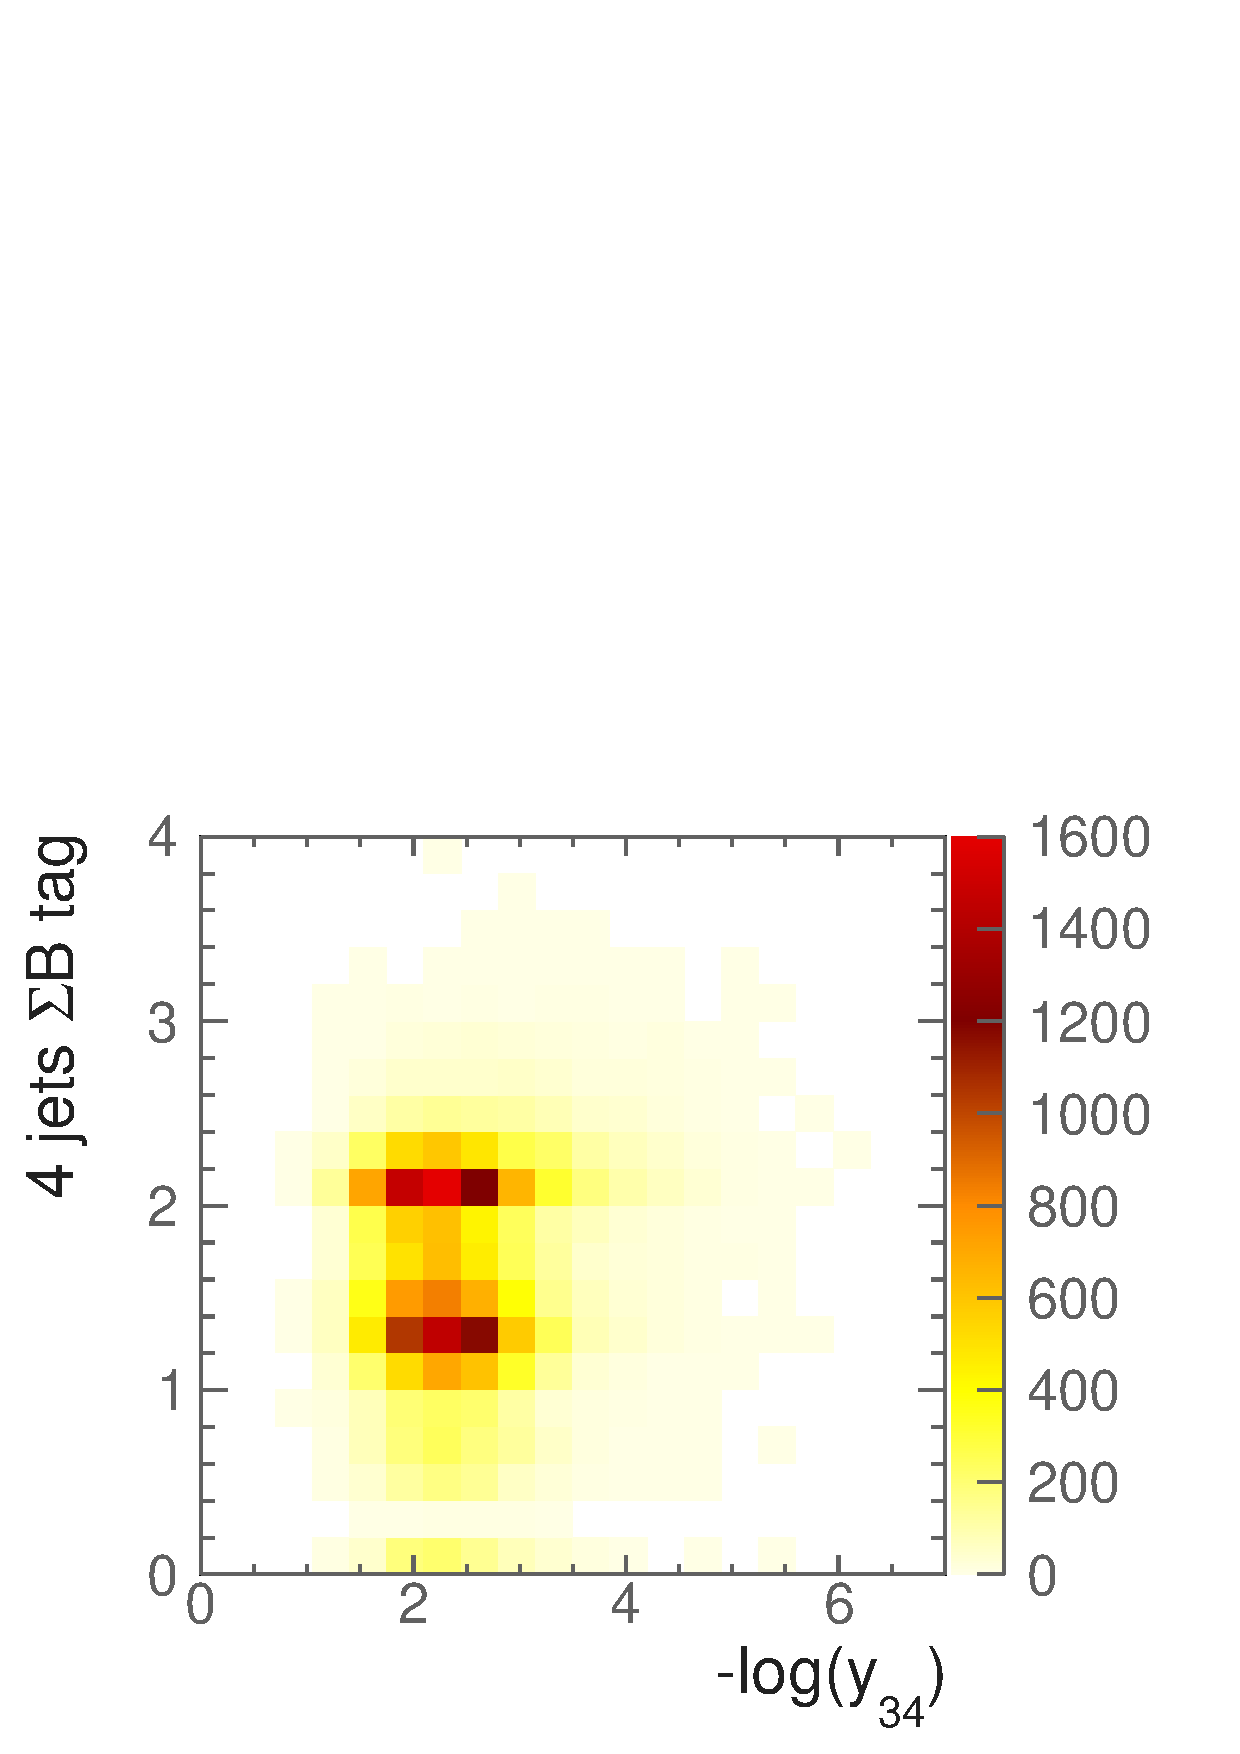
\includegraphics[width=\textwidth]{{doubleHiggs/mutual6022bbWW}.pdf}
    \caption{\eeToHHbbWW, hadronic}
    \label{fig:doubleHiggs1.4MutualbbWW}
  \end{subfigure}
    \begin{subfigure}[b]{0.45\textwidth}
    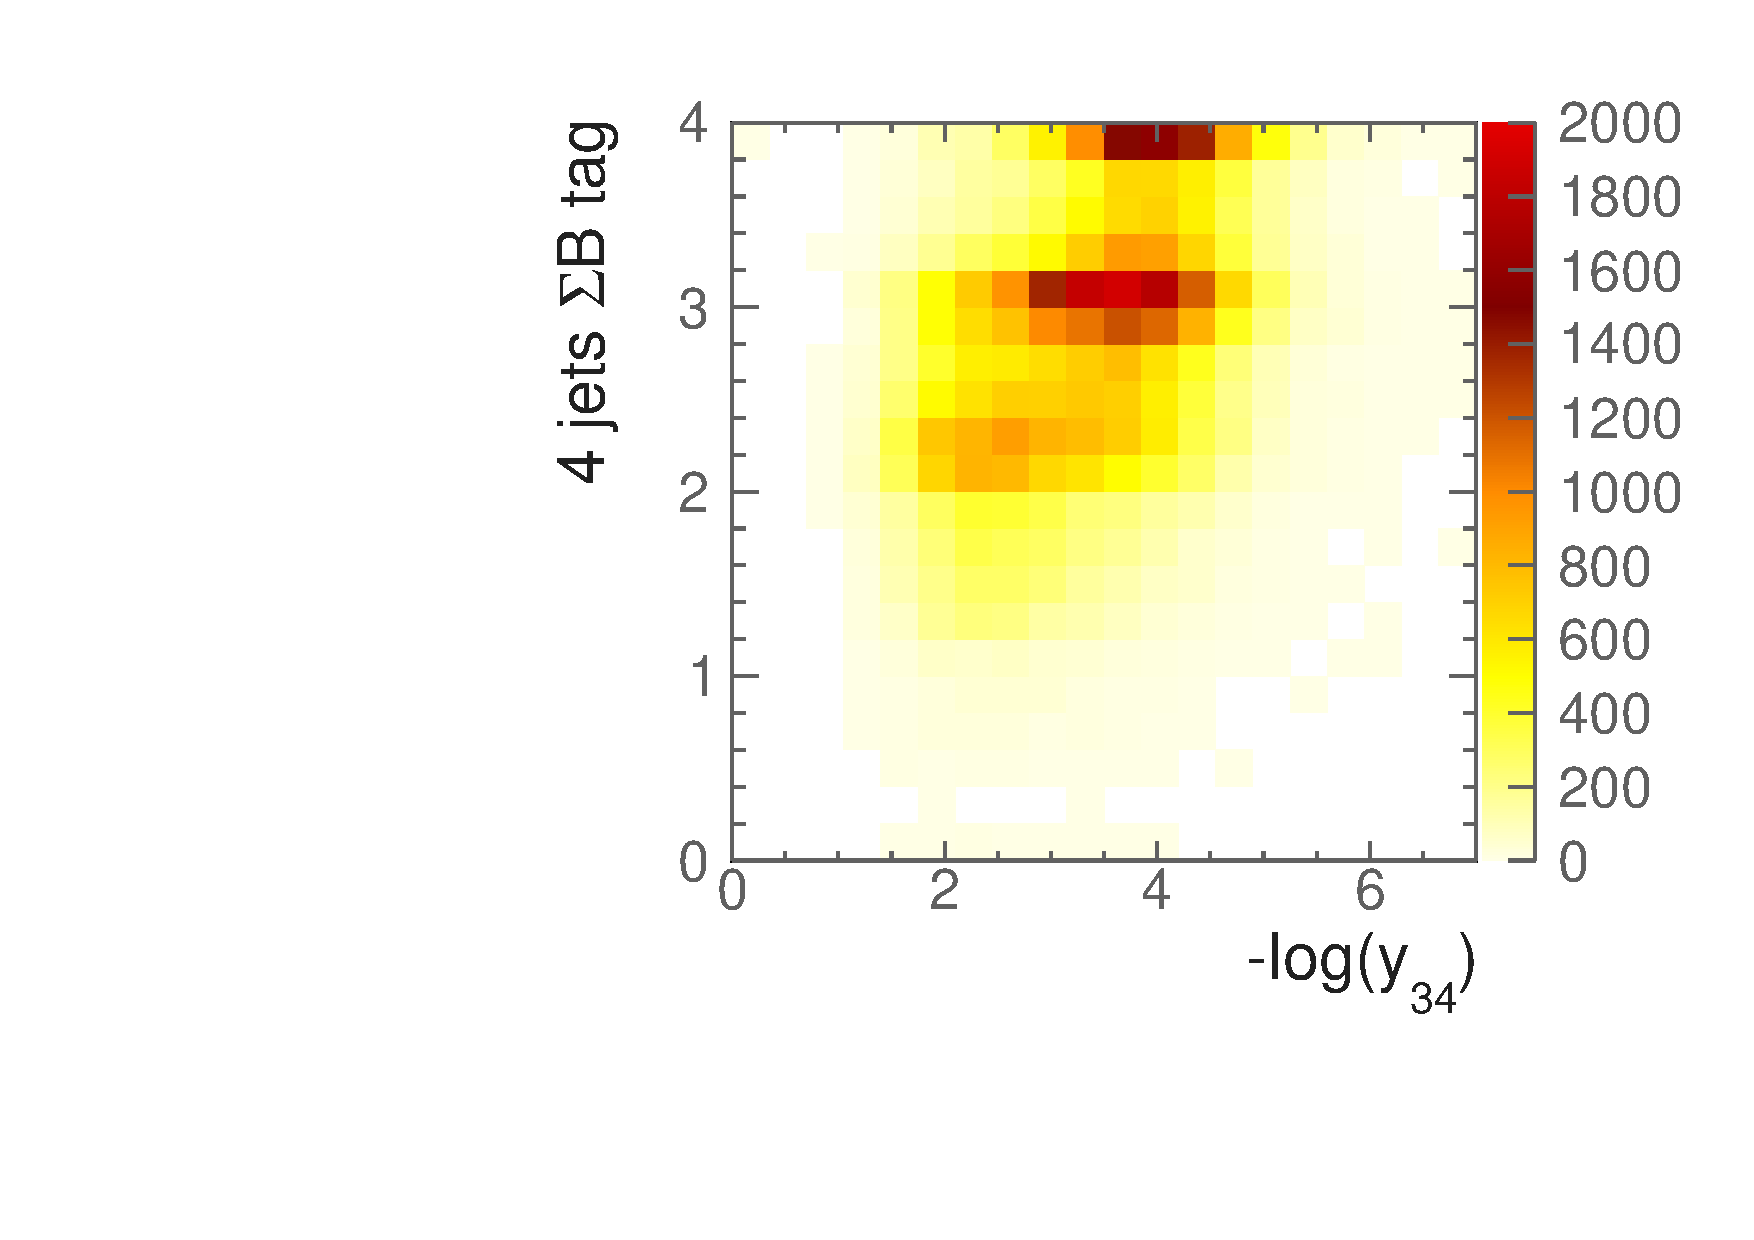
\includegraphics[width=\textwidth]{{doubleHiggs/mutual6022bbbb}.pdf}
    \caption{\eeToHHbbbb}
    \label{fig:doubleHiggs1.4Mutualbbbb}
  \end{subfigure}
\caption[Sum of b-jet tag values as a function of $-\log\parenths{\y{34}}$ at \rootS{1.4}]%
   {[Sum of b-jet tag values as a function of $-\log\parenths{\y{34}}$ at \rootS{1.4}, shown for hadronic decay of \eeToHHbbWW and \eeToHHbbWW sub-channel. }
   \label{fig:doubleHiggsMutualPreselection}
\end{figure}

\begin{table}[!tbp]
\centering
\begin{tabular}{lrr}
\hline
\hline
Selection efficiency & \multicolumn{1}{R{0.4\textwidth}}{\eeToHHbbWW, hadronic} & \multicolumn{1}{R{0.3\textwidth}}{\eeToHHbbbb} \\
\sumBtag{4} < 2.3 and \y{34} < 3.7 & 86\% & 78\% \\
\hline
\hline
\end{tabular}
\caption[Mutually exclusive cuts at \rootS{1.4}.] %
{Events passed mutually exclusive cuts at \rootS{1.4} for hadronic decay of \eeToHHbbWW and \eeToHHbbbb sub-channels.}
\label{tab:doubleHiggsMutualCuts}
\end{table}

The selection efficiencies of signal and background events after mutually exclusive cuts are listed in \Table{tab:doubleHiggsPreslectionPart2}. As designed, the mutually exclusive cuts reject most \eeToHHbbbb events.

\begin{table}[!tbp]\centering
\small
\begin{tabular}{lrr}
\hline \hline
 \multicolumn{1}{L{0.3\textwidth}}{Channel} &  \multicolumn{1}{R{0.3\textwidth}}{Previous cuts and loose cuts}  & \multicolumn{1}{R{0.3\textwidth}}{Mutually exclusive} \\
\hline
\eeToHH $\to$ \\
\HepProcess{ \Pbottom \APbottom \PWplus \PWminus \Pnue \APnue}, hadronic             & 66.4\%& 59.7\% \\
\hline
\eeToHH $\to$ \\
\HepProcess{ \Pbottom \APbottom \Pbottom \APbottom \Pnue \APnue}             &80.6\%& 15.4\%  \\
\eeToHH $\to$ other & 24.7\% & 20.5\%  \\
\hline
\eeTo{\qlight \qlight \PHiggs \Pnu \APnu}  & 42.0\% & 39.5\% \\
\eeTo{\Pcharm \APcharm \PHiggs \Pnu \APnu}  & 43.4\% & 31.7\%\\
\eeTo{\Pbottom \APbottom \PHiggs \Pnu \APnu}  & 64.2\% & 25.2\%\\

\eeTo{ \Pquark \Pquark \Pquark \Pquark}   & 4.6\%  & 3.4\%\\
\eeTo{ \Pquark \Pquark \Pquark \Pquark \Plepton \Plepton}& 3.3\% & 3.1\%\\
\eeTo{ \Pquark \Pquark \Pquark \Pquark \Plepton \Pnu}& 11.4\%. & 9.8\%\\
\eeTo{ \Pquark \Pquark \Pquark \Pquark \Pnu \APnu} & 18.8\% & 16.6\%\\

\eeTo{ \Pquark \Pquark} &  2.0\% & 0.8\%\\
\eeTo{ \Pquark \Pquark \Plepton \Pnu} &  1.6\% & 0.9\%\\
\eeTo{ \Pquark \Pquark \Pl \Pl} &  0.1\% & 0.1\%\\
\eeTo{ \Pquark \Pquark \Pnu \Pnu} & 5.8\% & 4.0\%\\
\hline
\egamma{\Pepm}{\Pphoton}{BS}{\Pepm \Pquark \Pquark \Pquark \Pquark} & 0.4\%  & 0.3\%\\
%\egamma{\Pem}{\Pphoton}{BS}{\Pem \Pquark \Pquark \Pquark \Pquark} & 0.4\%  & 0.3\%\\
%\egamma{\Pep}{\Pphoton}{BS}{\Pep \Pquark \Pquark \Pquark \Pquark} & 0.4\% & 0.4\%\\
\egamma{\Pepm}{\Pphoton}{EPA}{\Pepm \Pquark \Pquark \Pquark \Pquark} & 0.3\% & 0.2\%\\
%\egamma{\Pem}{\Pphoton}{EPA}{\Pem \Pquark \Pquark \Pquark \Pquark} & 0.3\% & 0.2\%\\
%\egamma{\Pep}{\Pphoton}{EPA}{\Pep \Pquark \Pquark \Pquark \Pquark}  & 0.3\% & 0.3\% \\
\egamma{\Pepm}{\Pphoton}{BS}{\Pnu \Pquark \Pquark \Pquark \Pquark}& 27.5\%  & 25.6\%\\
%\egamma{\Pem}{\Pphoton}{BS}{\Pnu \Pquark \Pquark \Pquark \Pquark}& 27.7\%  & 25.3\%\\
%\egamma{\Pep}{\Pphoton}{BS}{\APnu \Pquark \Pquark \Pquark \Pquark}& 27.3\% & 24.9\% \\
\egamma{\Pem}{\Pphoton}{EPA}{\Pnu \Pquark \Pquark \Pquark \Pquark}&  13.8\% & 12.5\% \\
%\egamma{\Pem}{\Pphoton}{EPA}{\Pnu \Pquark \Pquark \Pquark \Pquark}&  13.9\% & 12.6\% \\
%\egamma{\Pep}{\Pphoton}{EPA}{\APnu \Pquark \Pquark \Pquark \Pquark}& 13.7\%  & 12.3\% \\
\egamma{\Pepm}{\Pphoton}{BS}{\Pquark \Pquark \PHiggs \Pnu} & 34.6\%  & 30.6\% \\
%\egamma{\Pem}{\Pphoton}{BS}{\Pquark \Pquark \PHiggs \Pnu} & 34.6\%  & 30.6\% \\
%\egamma{\Pep}{\Pphoton}{BS}{\Pquark \Pquark \PHiggs \Pnu} & 34.6\% & 30.6\%  \\
\egamma{\Pem}{\Pphoton}{EPA}{\Pquark \Pquark \PHiggs \Pnu} & 18.3\% & 16.0\%  \\
%\egamma{\Pem}{\Pphoton}{EPA}{\Pquark \Pquark \PHiggs \Pnu} & 18.2\% & 16.0\%  \\
%\egamma{\Pep}{\Pphoton}{EPA}{\Pquark \Pquark \PHiggs \Pnu} & 18.4\%   & 16.1\%  \\
\hline
\gammagamma{\Pphoton}{BS}{\Pphoton}{BS}{ \Pquark \Pquark \Pquark \Pquark}& 0.3\%  & 0.3\%\\
\gammagamma{\Pphoton}{BS}{\Pphoton}{EPA}{ \Pquark \Pquark \Pquark \Pquark}& 0.4\%  &0.3\%\\
\gammagamma{\Pphoton}{EPA}{\Pphoton}{BS}{ \Pquark \Pquark \Pquark \Pquark}& 0.4\% & 0.3\%\\
\gammagamma{\Pphoton}{EPA}{\Pphoton}{EPA}{ \Pquark \Pquark \Pquark \Pquark}& 0.4\% & 0.3\% \\
\hline \hline
\end{tabular}
\caption[List of signal and background samples after loose cuts and mutually exclusive cuts at \rootS{1.4}.]
{List of signal and background samples after loose cuts and mutually exclusive cuts at \rootS{1.4}. The selection efficiencies are presented in a ``flow'' fashion. Every selection cut contains all the cuts to the left of it.}
\label{tab:doubleHiggsPreslectionPart2}
\end{table}


\begin{comment}
    const TCut selectionCut3000 = "tR0_7_6jet_btag2_ChiSquared<20  && TightIsoLepTauAll_nPfo < 1 && BonoForwardElectronPhotons_nPfo < 1 && \
         tR0_7_6jet_btag2_Higgs_all_M>150  && \
       tR0_7_4jet_btag2_Higgs_all_bTag < 2.3 && tR0_7_6jet_btag2_minusLogY34 < 3.7 \
       && tR0_7_6jet_btag2_bTag1 > 0.7 &&\
        tR0_7_6jet_btag2_Higgs_all_M  < 3000 &&  tR0_7_6jet_btag2_Higgs1_M < 500 &&  tR0_7_6jet_btag2_Higgs2_M < 800 &&  tR0_7_6jet_btag2_W_Onshell_M < 200";

    const TCut selectionCut1400 = "nR0_7_6jet_btag2_ChiSquared<20  && IsoLepTauAll_nPfo < 1      && BonoForwardElectronPhotons_nPfo < 1 && nR0_7_6jet_btag2_Higgs_all_M>150 && \
        nR0_7_4jet_btag2_Higgs_all_bTag < 2.3  && nR0_7_6jet_btag2_minusLogY34 < 3.6 \
        &&  nR0_7_6jet_btag2_bTag2 > 0.2 && nR0_7_6jet_btag2_Higgs_all_Pt> 30 &&\
        nR0_7_6jet_btag2_Higgs_all_M  < 1400 &&  nR0_7_6jet_btag2_Higgs1_M < 500 &&  nR0_7_6jet_btag2_Higgs2_M < 800 &&  nR0_7_6jet_btag2_W_Onshell_M < 200";
\end{comment}

\subsection{Cuts to aid the MVA}

A set of physics-motivated cuts aims to reduce the range of invariant masses variables in order to increase the effectiveness of the MVA. (See \Section{sec:pandoraMVAbdtVar}). The invariant masses of physical bosons are required to be within a certain range to avoid the effect of extreme values on the MVA. The cuts are listed in \Table{tab:doubleHiggsPreSel} and the performance is shown in \Figure{tab:doubleHiggsPreslectionPart2}.


The selection efficiencies of all pre-selection cuts are shown in \Table{tab:doubleHiggs1.4TeVPreslection}. As the signal cross section is small compared to the background, only the signal events with very clear characteristic topologies would be selected by the MVA. Therefore, pre-selection cuts would not be detrimental to the final signal selection. On the contrary, pre-selection cuts improve the final signal selection efficiency as the MVA can focus on the difficult background events where their topologies are similar to the signal events.


\section{Discriminative variables for MVA}

A series of discriminative variables are calculated to differentiate the signal and background events. These variables are fed into MVA for signal selection. A full list of variables can be found in \Table{tab:doubleHiggsVaraibles}.

Invariant mass of $m_{\Hbb}$ and $m_{\HWW}$ are very effective at selecting signal events as no background events have double Higgs bosons in final states. \FIGURE{fig:doubleHiggs1.4varMHbb} and \Figure{fig:doubleHiggs1.4varMHWW} show the distributions of $m_{\Hbb}$ and $m_{\HWW}$ after all pre-selection cuts.

For the off-shell \W*, its energy is used as its mass distribution does not have a resonance peak. The recoil momenta, which is calculated by assuming the collision at \sqrtS and a beam crossing angle of 20\,mrad. The pseudorapidity is used to describe the angle and focus on the forward region, defined as:
\begin{equation}
\eta \equiv  - \ln \left[ \tan \left( \frac{\theta}{2} \right) \right],
\end{equation}
where $\theta$ is the polar angle in a spherical polar coordinate system. Acollinearity, \acolinearity{12}, measures the angle between the two constituent jets, defined as:
\begin{equation}
\acolinearity{12} = \pi - \cos^{-1}\left(\textbf{\^{p}}_1\cdot\textbf{\^{p}}_2\right),
\end{equation}
where $\textbf{\^{p}}_1$ is the unit momentum three-vector of jet 1. \cosStar{12} is the cosine of the angle between the two constituent jets in their decay rest frame. \FIGURE{fig:doubleHiggs1.4varAcolHbb} and \Figure{fig:doubleHiggs1.4varSpinHbb} compares the \acolinearity{\Hbb} and  \cosStar{\Hbb}. Both show clear differences for the signal and background channels. For the signal, \cosStar{\Hbb} has a flat distribution, as expected from a back-to-back decay of \HepProcess{\PHiggs \to \Pbottom \APbottom}. For the background, \cosStar{\Hbb} peaks at 1.

The global event shape variables include \y{} variables (see \Section{sec:pandoraYparameter}), and the sphericity,  \sphericity. \sphericity is a measurement of the spherically symmetry of the event (see \Section{sec:pandoraEvtShape}).

The flavour tagging variables are discussed in \Section{sec:doubleHiggsFlavourTagging}. For example, \btagFull{1,\Hbb} denotes the highest b-jet tag value of two jets forming \Hbb. The number of \PFOs variables are effective against background events with fewer than six quarks in final states.

An optimal set of 32 variables are chosen for the best MVA performance, whilst no strong ($>80\%$) pair-wise correlation exists between any two variables. %shown in \Figure{fig:doubleHiggs1.4Corr}.


 \begin{table}[!tbp]\centering
\begin{tabular}{lr}
\hline
\hline
Category &  Variable \\
\hline
Invariant mass &  \multicolumn{1}{R{0.6\textwidth}}{$m_{\Hbb}$, $m_{\HWW}$, $m_{\PW}$, $m_{\HH}$} \\
Energy and momentum & \multicolumn{1}{R{0.6\textwidth}}{$E_{\W*}$, $E_{mis}$, $\pT_{\Hbb}$, $\pT_{\HWW}$, $\pT_{\PW}$, $\pT_{\HH}$} \\
Angles in lab frame & \multicolumn{1}{R{0.6\textwidth}}{$\eta_{mis}$, $\acolinearity{\Hbb}$, $\acolinearity{\PW}$, $\acolinearity{\HH}$} \\
Angles in boosted frames & \multicolumn{1}{R{0.6\textwidth}}{$\cosStar{\Hbb}$, $\cosStar{\HWW}$, $\cosStar{\PW}$, $\cosStar{\W*}$, $\cosStar{\HH}$} \\
Event shape & \multicolumn{1}{R{0.6\textwidth}}{$\abs{\sphericity}$, $-\ln(\y{23})$, $-\ln(\y{34})$, $-\ln(\y{45})$, $-\ln(\y{56})$} \\
\Pbottom and \Pcharm tag & \multicolumn{1}{R{0.6\textwidth}}{$\btagFull{1,\Hbb}$, $\btagFull{2,\Hbb}$, $\btagFull{1,\PW}$, $\btagFull{1,\W*}$, $\ctagFull{1,\Hbb}$, $\ctagFull{1,\PW}$} \\
Number of \PFOs &  \multicolumn{1}{R{0.6\textwidth}}{$\npfo{\Hbb}$, $\npfo{\HWW}$, $\npfo{\PW}$, $\npfo{\W*}$} \\
\hline
\hline
\end{tabular}
\caption
{Variables used in MVA at \rootS{1.4}}
\label{tab:doubleHiggsVaraibles}
\end{table}



 \begin{figure}[!tbp]
  \begin{subfigure}[b]{0.45\textwidth}
    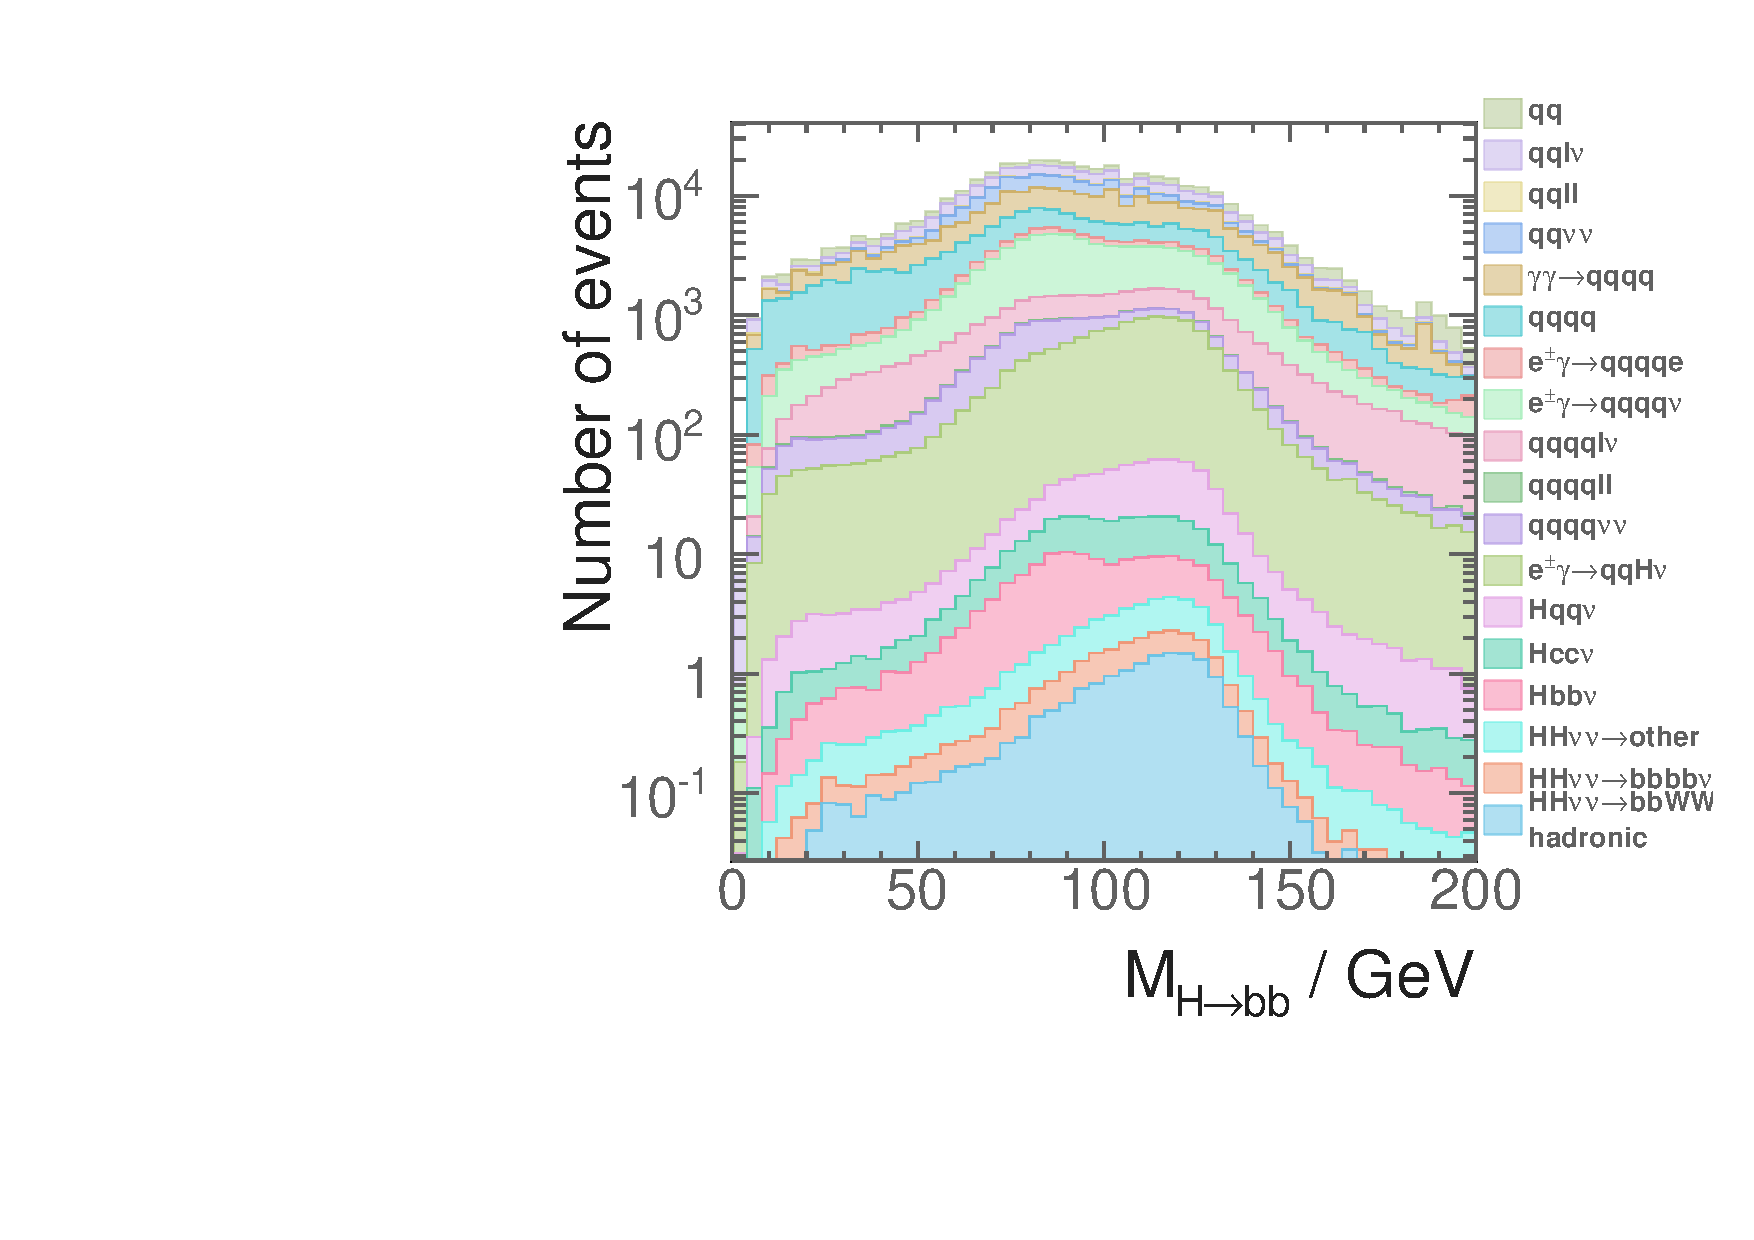
\includegraphics[width=\textwidth]{{doubleHiggs/1400var/nR0_7_6jet_btag2_Higgs1_M_TMVA20161208R0_7_qq_btag2_prepare_testNew2}.pdf}
    \caption{}
    \label{fig:doubleHiggs1.4varMHbb}
  \end{subfigure}
    \begin{subfigure}[b]{0.45\textwidth}
    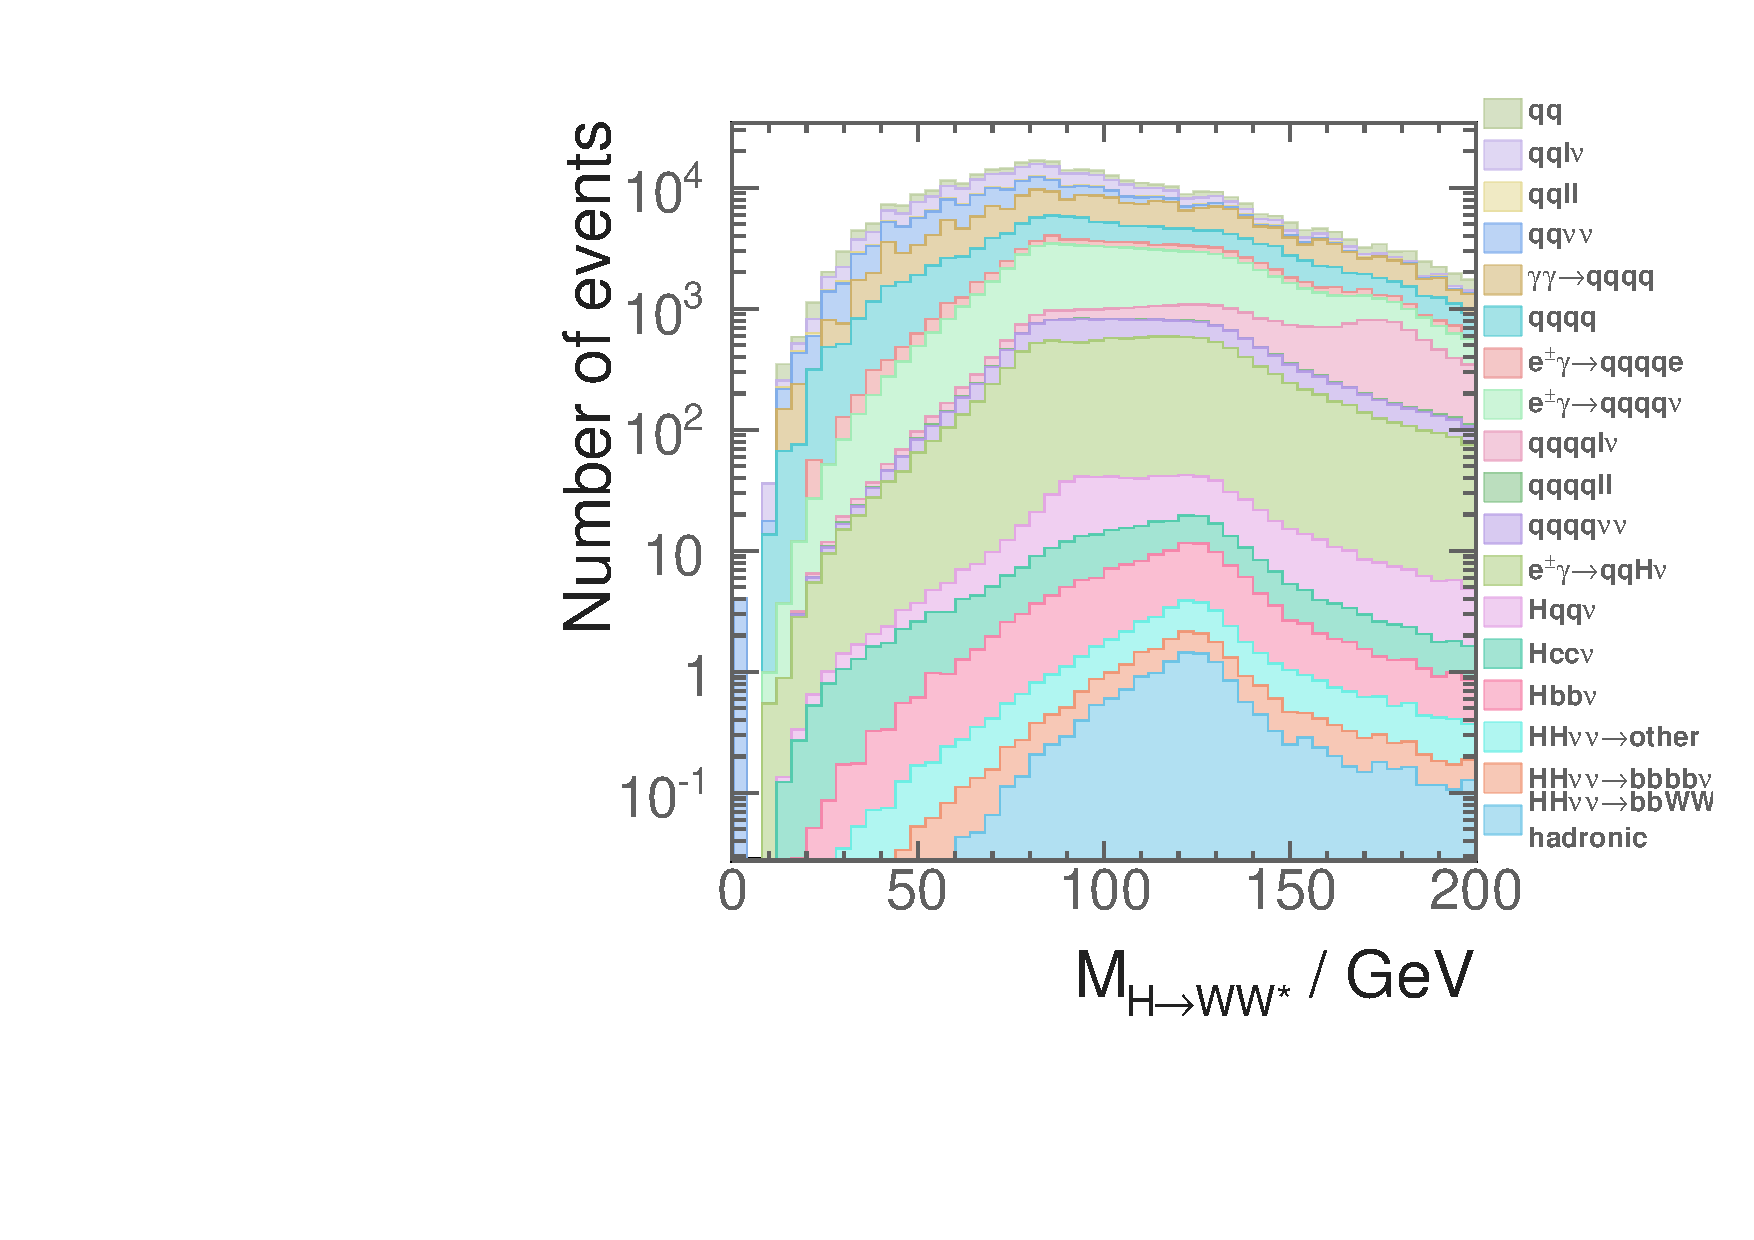
\includegraphics[width=\textwidth]{{doubleHiggs/1400var/nR0_7_6jet_btag2_Higgs2_M_TMVA20161208R0_7_qq_btag2_prepare_testNew2}.pdf}
    \caption{}
    \label{fig:doubleHiggs1.4varMHWW}
  \end{subfigure}
    \begin{subfigure}[b]{0.45\textwidth}
    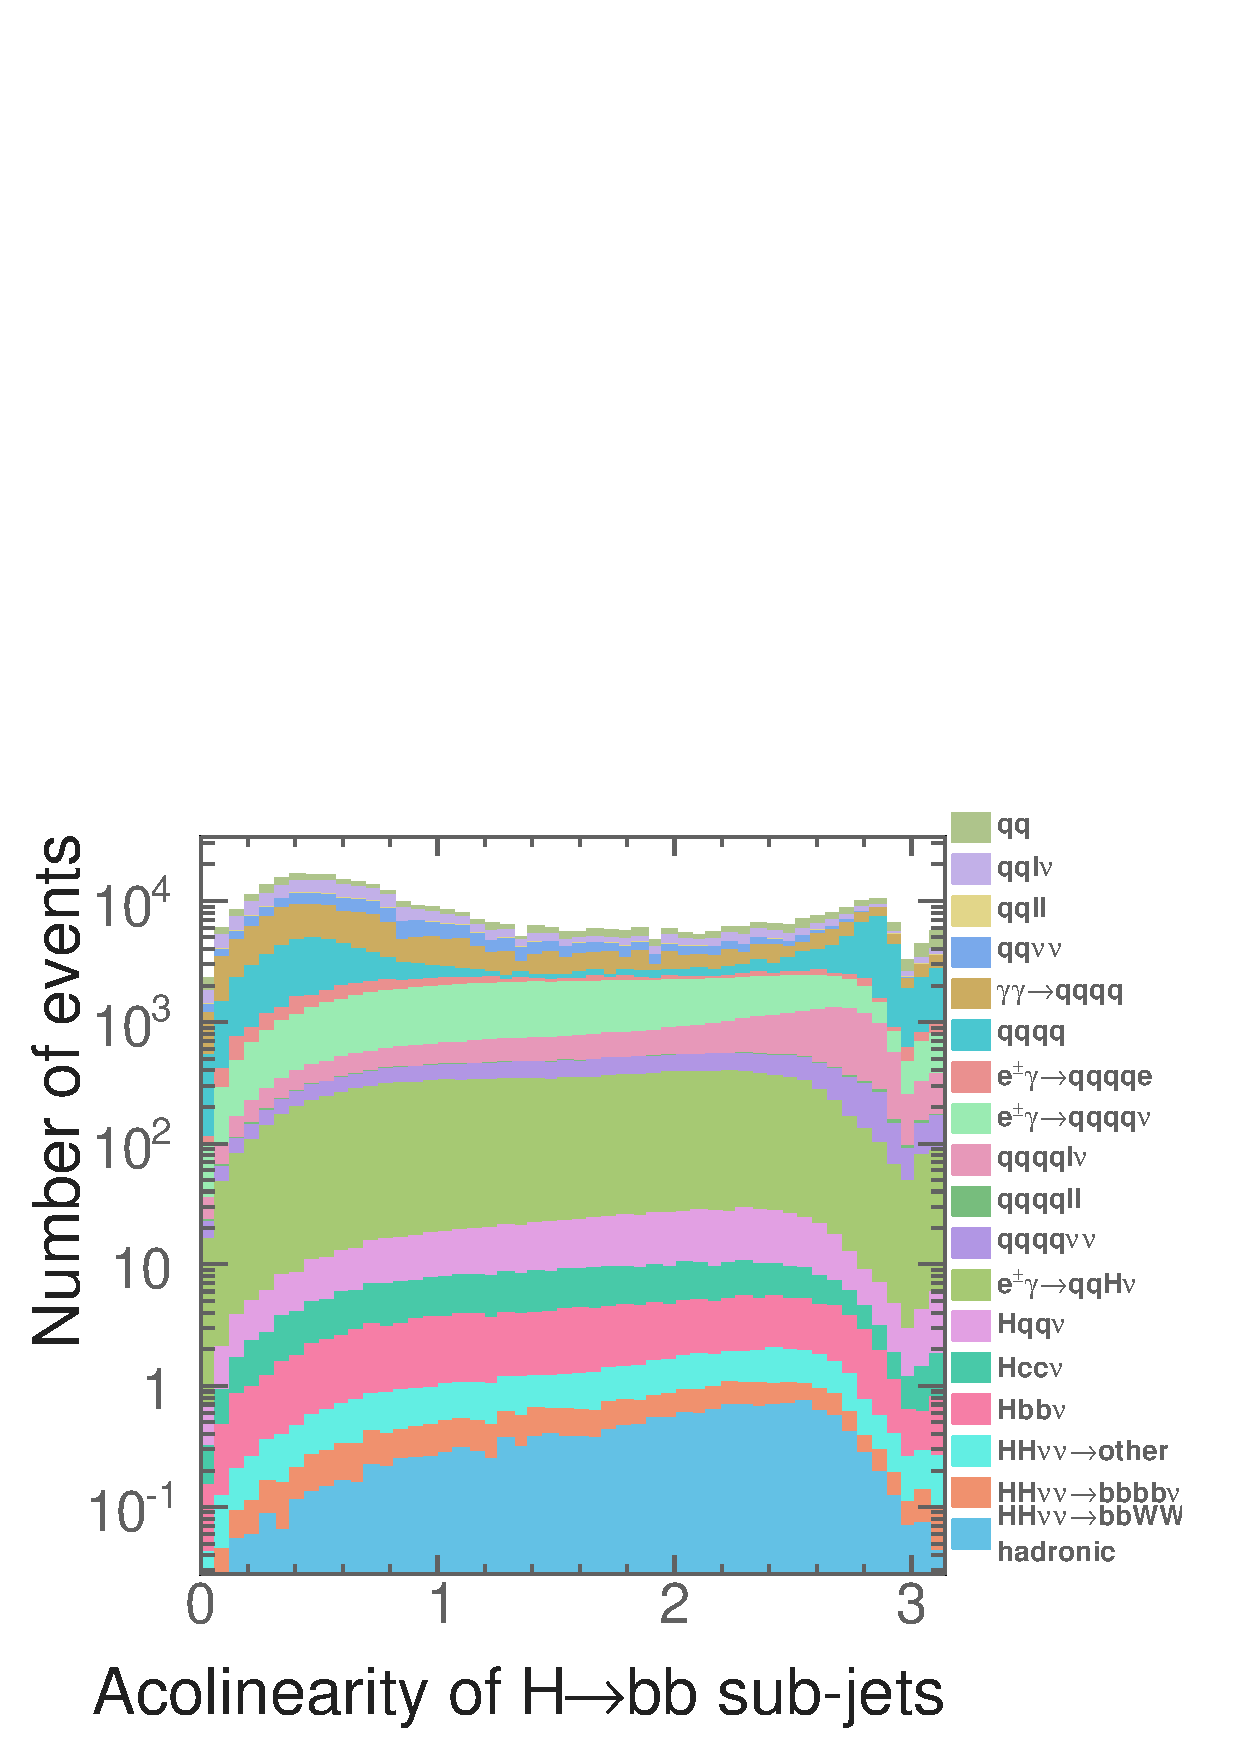
\includegraphics[width=\textwidth]{{doubleHiggs/1400var/nR0_7_6jet_btag2_Higgs1_acolinearity_TMVA20161208R0_7_qq_btag2_prepare_testNew2}.pdf}
    \caption{}
    \label{fig:doubleHiggs1.4varAcolHbb}
  \end{subfigure}
    \begin{subfigure}[b]{0.45\textwidth}
    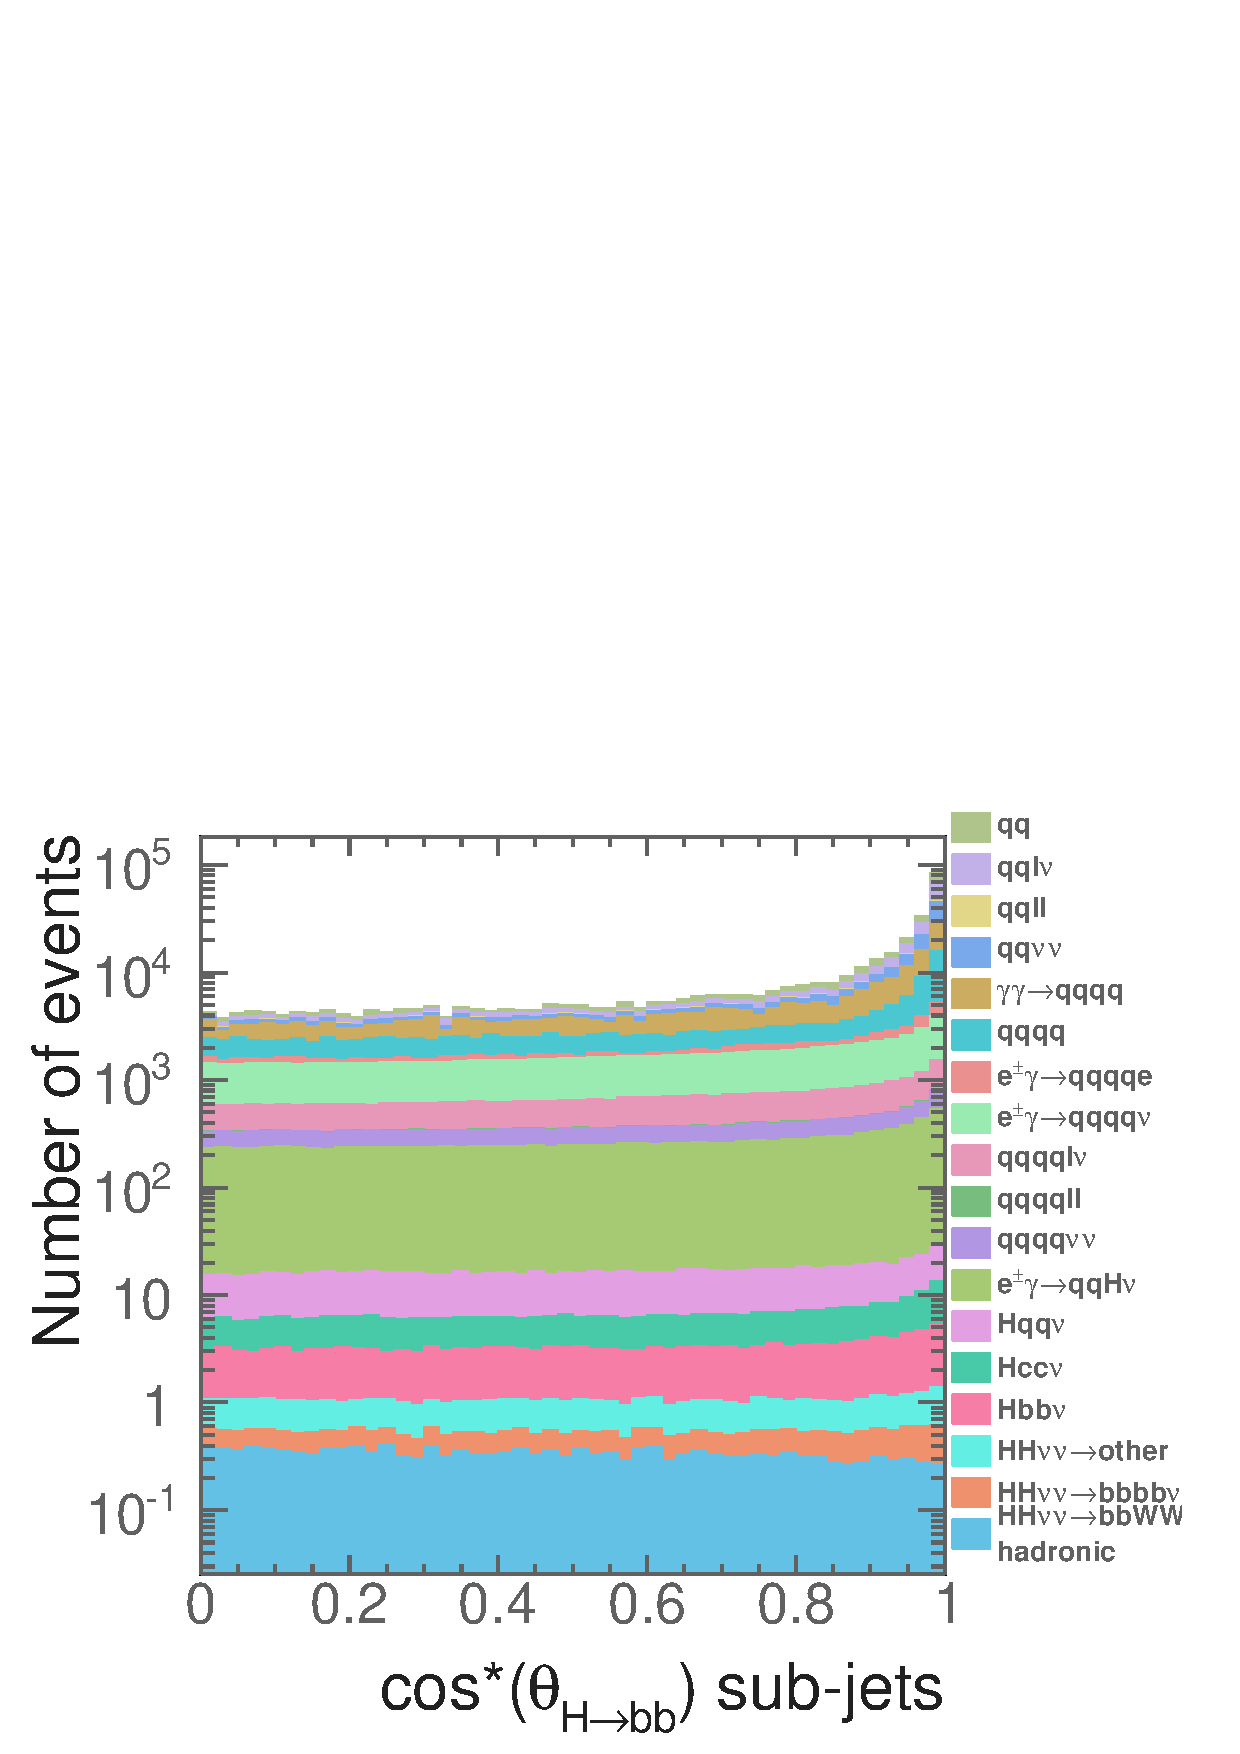
\includegraphics[width=\textwidth]{{doubleHiggs/1400var/nR0_7_6jet_btag2_Higgs1_spin_TMVA20161208R0_7_qq_btag2_prepare_testNew2}.pdf}
    \caption{}
    \label{fig:doubleHiggs1.4varSpinHbb}
  \end{subfigure}
\caption[Stacked plots of discriminative variables distributions used in the MVA at \rootS{1.4} after all pre-MVA cuts.]
   {Stacked plots of discriminative variables distributions used in the MVA at \rootS{1.4} after all pre-MVA cuts. \FIGURE{fig:doubleHiggs1.4varMHbb} and \Figure{fig:doubleHiggs1.4varMHWW} show the invariant mass distributions of \Hbb and \HWW. \FIGURE{fig:doubleHiggs1.4varAcolHbb} and \Figure{fig:doubleHiggs1.4varSpinHbb} show the acollinearity and the opening angle in the decay rest frame of the two jets forming \Hbb.}
   \label{fig:doubleHiggs1.4var}
\end{figure}

\begin{comment}
 \begin{figure}[!tbp]
  \begin{subfigure}[b]{0.45\textwidth}
    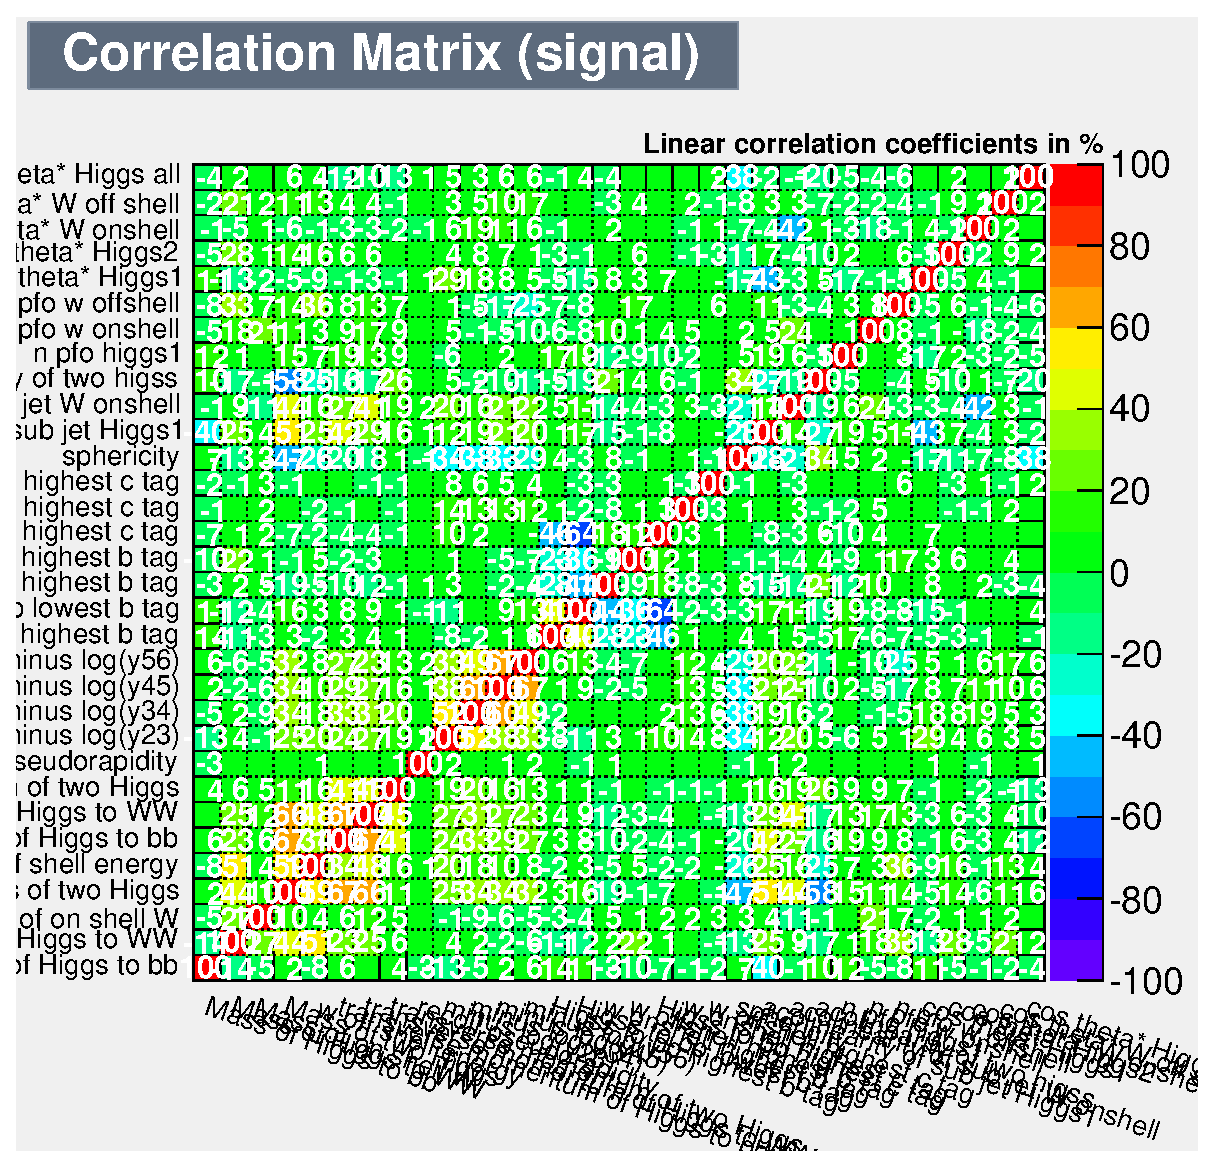
\includegraphics[width=\textwidth]{{doubleHiggs/mva/1400signalCorr}}
    \caption{}
    \label{fig:doubleHiggs1.4signalCorr}
  \end{subfigure}
    \begin{subfigure}[b]{0.45\textwidth}
    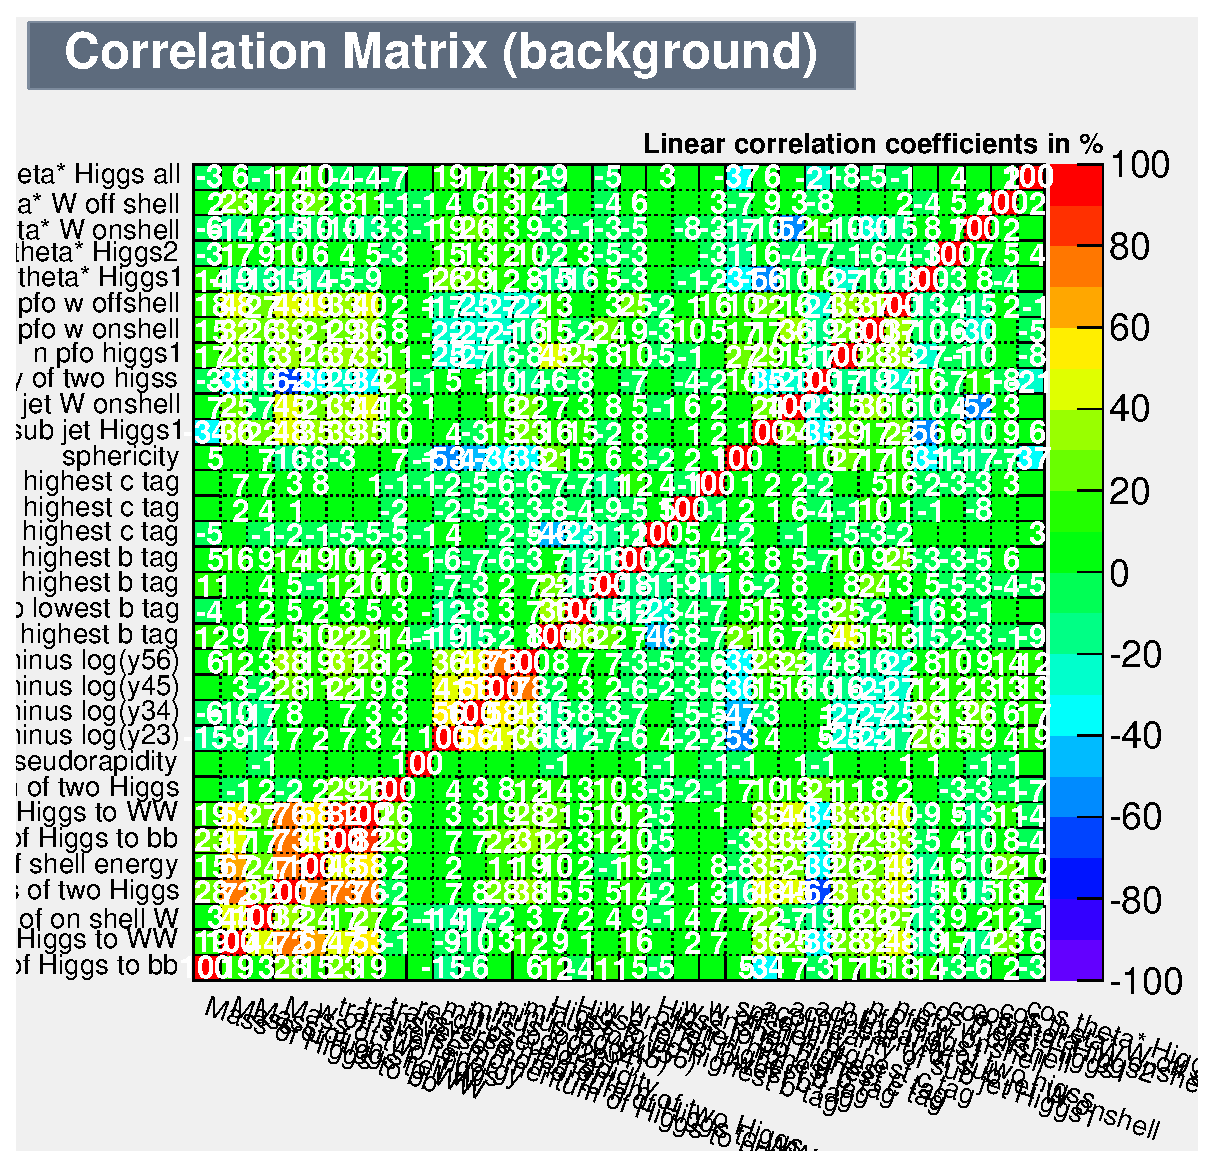
\includegraphics[width=\textwidth]{{doubleHiggs/mva/1400backgroundCorr}}
    \caption{}
    \label{fig:doubleHiggs1.4backgroundCorr}
  \end{subfigure}
\caption
   {The pair-wise correlation between discriminative variables for signal and background events at \rootS{1.4} after all pre-selection cuts.}
   \label{fig:doubleHiggs1.4Corr}
\end{figure}
\end{comment}

\section{Multivariate analysis}
\label{sec:doubleHiggsMVA}
After gathering information and applying  pre-selection cuts, signal events selection is performed using the multivariate analysis (MVA) with Boosted Decision Tree classifier (BDT). The parameters for boosted decision tree are optimised and checked for overtraining. A brief discussion on the MVA, classifier, and overtraining can be found in \Section{sec:pandoraMVA}.

The optimisation of the BDT follows the strategy outlined in \Section{sec:pandoraMVAbdtVar}. The optimised parameters are listed in \Table{tab:doubleHiggsBDTparameters}. The optimal values are obtained by choosing the best performance without overfitting.
%at \rootS{3}. The same optimised parameters are used for \rootS{1.4} analysis.

\begin{table}[!tbp]\centering
%\small{
\small
\begin{tabular}{lr}
\hline \hline
 Parameter &  Value \\
\hline
Depth of tree & 4 \\
Number of trees & 4000 \\
The minimum number of events in a node &  0.25\% of the total events \\
Boosting & adaptive boost \\
Learning rate of the adaptive boost & 0.5 \\
Metric for the optimal cuts & Gini Index \\
Bagging fraction & 0.5 \\
Number of bins per variables & 40 \\
End node output & x $\in [0,1]$ \\
Do-PreSelection & yes \\
\hline \hline
\end{tabular}

\caption
{Optimised parameters for the boosted decision tree classifier. See \Section{sec:pandoraMVAbdtVar} for detailed explanation of variables.}
\label{tab:doubleHiggsBDTparameters}
\end{table}

\begin{comment}
  "!H:!V:NTrees=4000:MinNodeSize=0.25%:MaxDepth=4:BoostType=RealAdaBoost:AdaBoostBeta=0.5:UseBaggedBoost:BaggedSampleFraction=0.5:SeparationType=GiniIndex:nCuts=40:DoPreselection=True" );
\end{comment}

Half of the samples were used for training, and the other half used for testing and classifier optimisation. The signal for the MVA is the hadronic decay of \eeToHH $\to$ \HepProcess{ \Pbottom \APbottom \PWplus \PWminus \Pnue \APnue}. \eeToHH decaying to other final states does not participate in the MVA training step. Although they are from the Feynman diagrams as the signal (see \Section{fig:doubleHiggsFeynman}), event topologies are different. They participate in the MVA applying stage.

\section{Signal selection results}
\label{sec:doubleHiggsSignalSelResult}
%first sentence doesn't make sense. Should there be an "and" in there?

Efficiencies of events passed the pre-selection cut and the MVA classifier are listed in \Table{tab:doubleHiggs1.4TeVMVA}, alongside with number of events after the MVA selection. A few  background channels have non-zero events after the MVA selection. \eeTo{\Pquark \APquark \PHiggs \Pnu \APnu} is difficult to discard because its topology, one single Higgs plus neutrino, is very similar to the signal event topology. Similarly, \eeTo{ \Pquark \Pquark \Pquark \Pquark \Plepton \Pnu} can be confused as the signal when the lepton is undetected in the forward region, or the lepton's energy is too low to be tagged. \eeTo{ \Pquark \Pquark \Pquark \Pquark \Pnu \APnu} can also have a similar topology to the signal. Other background channels that are not discarded after the MVA are the electron-photon and photon interactions with the same final states as the above channels.



Before interpreting the result at \rootS{1.4}, the analyses at \rootS{3} and  the semi-leptonic channel of \eeToHH $\to$ \HepProcess{ \Pbottom \APbottom \PWplus \PWminus \Pnue \APnue} are presented.

\begin{table}[!tbp]\centering
%\small{
\small
\begin{tabular}{lrrrr}
\hline \hline
 \multicolumn{1}{m{3.5cm}}{Channel / Efficiency \rootS{1.4}} &  \multicolumn{1}{m{2cm}}{N}  & \multicolumn{1}{m{2cm}}{$\varepsilon_{presel}$} & \multicolumn{1}{m{2cm}}{$\varepsilon_{MVA}$} & \multicolumn{1}{m{2cm}}{$N_{MVA}$} \\
\hline
\eeToHH $\to$ \\
\HepProcess{ \Pbottom \APbottom \PWplus \PWminus \Pnue \APnue}, hadronic             &27.9& 59.8\% & 8.2\% & 1.29 \\
\hline
\eeToHH $\to$ \\
\HepProcess{ \Pbottom \APbottom \Pbottom \APbottom \Pnue \APnue}             &67.6& 15.4\%  & 0.5\% & 0.05\\
\eeToHH $\to$ other                             & 128.0 & 20.4\% & 1.7\% & 0.45\\
\hline
\eeTo{\qlight \qlight \PHiggs \Pnu \APnu}  & 1304.0 & 39.5\% & 0.05\%& 0.29\\
\eeTo{\Pcharm \APcharm \PHiggs \Pnu \APnu}  & 546.1 & 31.6\%& 0.1\%& 0.16\\
\eeTo{\Pbottom \APbottom \PHiggs \Pnu \APnu}  & 463.0 & 24.7\%& 0.3\%& 0.37\\

\eeTo{ \Pquark \Pquark \Pquark \Pquark}   &   1867650.0& 3.3\% & - & -\\
\eeTo{ \Pquark \Pquark \Pquark \Pquark \Plepton \Plepton}& 93150.0 & 0.3\%& - &  - \\
\eeTo{ \Pquark \Pquark \Pquark \Pquark \Plepton \Pnu}& 165600.0 & 9.8\%& 0.01\%& 2.06\\
\eeTo{ \Pquark \Pquark \Pquark \Pquark \Pnu \APnu} & 34800.0& 16.5\%& 0.002\% & 0.10\\

\eeTo{ \Pquark \Pquark} &  6014250.0 & 0.8\%& - & - \\
\eeTo{ \Pquark \Pquark \Plepton \Pnu} &  6464550.0 & 0.9\%&  - & - \\
\eeTo{ \Pquark \Pquark \Pl \Pl} &  4088700.0 & 0.08\%& - & - \\
\eeTo{ \Pquark \Pquark \Pnu \Pnu} & 1181550.0 & 4.0\%& - & - \\
\hline
\egamma{\Pepm}{\Pphoton}{BS}{\Pepm \Pquark \Pquark \Pquark \Pquark} & 2606625.0  & 0.3\%& - & -\\
%\egamma{\Pem}{\Pphoton}{BS}{\Pem \Pquark \Pquark \Pquark \Pquark} & 1305787.5  & 0.3\%& - & -\\
%\egamma{\Pep}{\Pphoton}{BS}{\Pep \Pquark \Pquark \Pquark \Pquark} & 1300837.5 & 0.4\%& -& -\\
\egamma{\Pepm}{\Pphoton}{EPA}{\Pepm \Pquark \Pquark \Pquark \Pquark} & 861000.0 & 0.3\%&  - &  - \\
%\egamma{\Pem}{\Pphoton}{EPA}{\Pem \Pquark \Pquark \Pquark \Pquark} & 430650.0 & 0.3\%&  - &  - \\
%\egamma{\Pep}{\Pphoton}{EPA}{\Pep \Pquark \Pquark \Pquark \Pquark}  & 430350.0 & 0.3\% & - & -\\
\egamma{\Pepm}{\Pphoton}{BS}{\Pnu \Pquark \Pquark \Pquark \Pquark}& 178987.5  & 25.7\%& 0.005\%& 2.05\\
%\egamma{\Pem}{\Pphoton}{BS}{\Pnu \Pquark \Pquark \Pquark \Pquark}& 89775.0  & 25.4\%& 0.005\%& 1.09\\
%\egamma{\Pep}{\Pphoton}{BS}{\APnu \Pquark \Pquark \Pquark \Pquark}& 89212.5 & 24.9\% & 0.004\%& 0.96\\
\egamma{\Pepm}{\Pphoton}{EPA}{\Pnu \Pquark \Pquark \Pquark \Pquark}& 52050.0  & 12.5\% & 0.004\% & 0.27 \\
%\egamma{\Pem}{\Pphoton}{EPA}{\Pnu \Pquark \Pquark \Pquark \Pquark}& 26100.0  & 12.6\% & - &  - \\
%\egamma{\Pep}{\Pphoton}{EPA}{\APnu \Pquark \Pquark \Pquark \Pquark}& 25950.0  & 12.4\%& 0.008\% & 0.27\\
\egamma{\Pepm}{\Pphoton}{BS}{\Pquark \Pquark \PHiggs \Pnu} & 35437.5   & 30.7\% & 0.02\% & 2.16 \\
%\egamma{\Pem}{\Pphoton}{BS}{\Pquark \Pquark \PHiggs \Pnu} & 17775   & 30.8\% & 0.02\% & 1.00 \\
%\egamma{\Pep}{\Pphoton}{BS}{\Pquark \Pquark \PHiggs \Pnu} & 17662.5  & 30.6\% & 0.02\% & 1.16 \\
\egamma{\Pepm}{\Pphoton}{EPA}{\Pquark \Pquark \PHiggs \Pnu} & 10170.0  & 16.1\% & 0.06\% & 0.95 \\
%\egamma{\Pem}{\Pphoton}{EPA}{\Pquark \Pquark \PHiggs \Pnu} & 5085  & 16.0\% & 0.04\% & 0.33 \\
%\egamma{\Pep}{\Pphoton}{EPA}{\Pquark \Pquark \PHiggs \Pnu} & 5085   & 16.2\% & 0.08\% & 0.62 \\
\hline
\gammagamma{\Pphoton}{BS}{\Pphoton}{BS}{ \Pquark \Pquark \Pquark \Pquark}& 2054951.5  & 0.2\%&  - & -\\
\gammagamma{\Pphoton}{BS}{\Pphoton}{EPA}{ \Pquark \Pquark \Pquark \Pquark}& 4521037.5  & 0.4\%& - & - \\
\gammagamma{\Pphoton}{EPA}{\Pphoton}{BS}{ \Pquark \Pquark \Pquark \Pquark}& 4539150.0 & 0.3\%&  - & - \\
\gammagamma{\Pphoton}{EPA}{\Pphoton}{EPA}{ \Pquark \Pquark \Pquark \Pquark}& 1129500.0 & 0.3\% & - & -\\
\hline \hline
\end{tabular}

\caption[Selection efficiency and number of events for signal and background at \rootS{1.4}.]%
{List of signal and background samples with selection efficiency and number of events at \rootS{1.4}, assuming a luminosity of 1500$fb^{-1}$. The number of events, selection efficiency of pre-selection, selection efficiency of MVA after pre-selection, number of events after MVA are shown. - represents a number less than 0.01.}
\label{tab:doubleHiggs1.4TeVMVA}
\end{table}



\section{\eeToHH $\to$ \HepProcess{ \Pbottom \APbottom \PWplus \PWminus \Pnu \APnu} hadronic decay at \rootS{3} analysis}

The \eeToHH $\to$ \HepProcess{ \Pbottom \APbottom \PWplus \PWminus \Pnu \APnu} hadronic decay at \rootS{3} analysis follows the same strategy as the analysis at \rootS{1.4}. A brief discussion of each step and the results are provided and differences are highlighted. Cross sections of used samples are listed in \Table{tab:doubleHiggs3crossSection}.

\begin{table}[!tbp]\centering
% TODO fix lumi correction for e gamma, gamma e
% TODO change some of sample cross section for  electron-photon interaction with four quarks and a neutrino final state
\small
%{

\begin{tabular}{lrr}
\hline \hline
Channel  &  $\sigma(\rootS{3})$ / fb   \\
\hline
\eeToHH &0.588 \\
\hline
\eeToHHbbWWFull,hadronic &0.07 \\
\eeToHHbbbbFull  &0.19 \\
\eeToHHotherFull &0.34 \\
\hline
\eeTo{\qlight \qlight \PHiggs \Pnu \APnu} & 1.78 \\
\eeTo{\Pcharm \APcharm \PHiggs \Pnu \APnu} & 1.12\\
\eeTo{\Pbottom \APbottom \PHiggs \Pnu \APnu}  & 1.91\\

\eeTo{ \Pquark \Pquark \Pquark \Pquark} & 546.5*\\
\eeTo{ \Pquark \Pquark \Pquark \Pquark \Plepton \Plepton}&169.3*\\
\eeTo{ \Pquark \Pquark \Pquark \Pquark \Plepton \Pnu} &106.6*\\
\eeTo{ \Pquark \Pquark \Pquark \Pquark \Pnu \APnu}&71.5*\\

\eeTo{ \Pquark \Pquark} &2948.9\\
\eeTo{ \Pquark \Pquark \Plepton \Pnu} &5561.1\\
\eeTo{ \Pquark \Pquark \Pl \Pl}&3319.6\\
\eeTo{ \Pquark \Pquark \Pnu \Pnu} &1317.5 \\
\hline
\egamma{\Pepm}{\Pphoton}{BS}{\Pepm \Pquark \Pquark \Pquark \Pquark} & 2536.3*\\
%\egamma{\Pem}{\Pphoton}{BS}{\Pem \Pquark \Pquark \Pquark \Pquark} & 1268.7*\\
%\egamma{\Pep}{\Pphoton}{BS}{\Pep \Pquark \Pquark \Pquark \Pquark}  & 1267.6*\\
\egamma{\Pepm}{\Pphoton}{EPA}{\Pepm \Pquark \Pquark \Pquark \Pquark}  & 575.7*\\
%\egamma{\Pem}{\Pphoton}{EPA}{\Pem \Pquark \Pquark \Pquark \Pquark}  & 287.9*\\
%\egamma{\Pep}{\Pphoton}{EPA}{\Pep \Pquark \Pquark \Pquark \Pquark}   & 287.8*\\
\egamma{\Pepm}{\Pphoton}{BS}{\Pnu \Pquark \Pquark \Pquark \Pquark}  & 524.8*\\
%\egamma{\Pem}{\Pphoton}{BS}{\Pnu \Pquark \Pquark \Pquark \Pquark}  & 262.5*\\
%\egamma{\Pep}{\Pphoton}{BS}{\APnu \Pquark \Pquark \Pquark \Pquark} & 262.3*\\
\egamma{\Pepm}{\Pphoton}{EPA}{\Pnu \Pquark \Pquark \Pquark \Pquark}  & 108.4*\\
%\egamma{\Pem}{\Pphoton}{EPA}{\Pnu \Pquark \Pquark \Pquark \Pquark}  & 54.2*\\
%\egamma{\Pep}{\Pphoton}{EPA}{\APnu \Pquark \Pquark \Pquark \Pquark}& 54.2*\\
\egamma{\Pepm}{\Pphoton}{BS}{\Pquark \Pquark \PHiggs \Pnu}   & 117.1* \\
%\egamma{\Pem}{\Pphoton}{BS}{\Pquark \Pquark \PHiggs \Pnu}   & 58.6* \\
%\egamma{\Pep}{\Pphoton}{BS}{\Pquark \Pquark \PHiggs \Pnu}  & 58.5* \\
\egamma{\Pepm}{\Pphoton}{EPA}{\Pquark \Pquark \PHiggs \Pnu} & 22.4* \\
%\egamma{\Pem}{\Pphoton}{EPA}{\Pquark \Pquark \PHiggs \Pnu} & 11.7* \\
%\egamma{\Pep}{\Pphoton}{EPA}{\Pquark \Pquark \PHiggs \Pnu} & 11.7* \\
\hline
\gammagamma{\Pphoton}{BS}{\Pphoton}{BS}{ \Pquark \Pquark \Pquark \Pquark}&13050.3*\\
\gammagamma{\Pphoton}{BS}{\Pphoton}{EPA}{ \Pquark \Pquark \Pquark \Pquark}&2420.6*\\
\gammagamma{\Pphoton}{EPA}{\Pphoton}{BS}{ \Pquark \Pquark \Pquark \Pquark}&2423.1*\\
\gammagamma{\Pphoton}{EPA}{\Pphoton}{EPA}{ \Pquark \Pquark \Pquark \Pquark}&402.7* \\
\hline \hline
\end{tabular}

\caption[Cross sections of samples at \rootS{3}.]
{List of signal and background samples with the corresponding cross sections at \rootS{3}. \Pquark can be \Pup, \Pdown, \Pstrange, \Pbottom or \Ptop. Unless specified, \Pquark, \Plepton and \Pnu represent particles and their corresponding anti-particles. \Pphoton(BS) represents a real photon from beamsstrahlung (BS). \Pphoton(EPA) represents a ``quasi-real'' photon simulated with the Equivalent Photon Approximation. For processes involving Higgs production explicitly, simulated Higgs mass is 126\,GeV. Otherwise, Higgs mass is set to 14\,TeV. For processes labelled with *, the generator level cut requires invariant mass of quarks greater than 50\,GeV.}
\label{tab:doubleHiggs3crossSection}
\end{table}

The lepton finding processors are either developed or optimised with samples at \rootS{1.4}, and checked with samples at \rootS{3} (see \Section{sec:doubleHiggsLepton}).  It was found that the same set of parameters for lepton identifiers works well under \rootS{1.4} and 3\,TeV. The performance of the lepton processors is shown in \Table{tab:doubleHiggs3TeVIsoLepPerformance}.

\begin{table}[!tbp]
\begin{tabular}{lrr}
\hline
\hline
Efficiency (3\,TeV)  &  Signal  & \HepProcess{\Pep \Pem \to \Pquark\Pquark\Pquark\Pquark\Plepton\Pnu} \\
\hline
\IsolatedLeptonFinderProcessor & 99.5\% & 66.8\%  \\
\BonoLeptonFinder & 99.0\% & 52.5\%  \\
\TauFinderProcessor & 97.7\% & 79.5\%  \\
\BonoTauFinder & 86.3\% & 60.3\%  \\
Forward Finder Processors & 95.9\% & 80.7\%  \\
\hline
Combined & 81.0\% & 23.3\%  \\
\hline
\hline

\end{tabular}
\caption{Isolated lepton finder processors performance with the signal and selected background samples at \rootS{3}.}
\label{tab:doubleHiggs3TeVIsoLepPerformance}
\end{table}

%Would this read better if you explained why 1.4 is better rather than why 3 is worse? Better should be the focus, no?
When comparing \rootS{1.4} and \rootS{3}, the lepton finding performance is better for \rootS{1.4}. This is because at \rootS{3}, particles are  boosted and spatial separation between particles is smaller. The effect of high \sqrtS also reflects on the performance of the  ForwardFinderProcessor. Whilst at \rootS{1.4}, the processor only rejects 5\% \HepProcess{\Pep \Pem \to \Pquark\Pquark\Pquark\Pquark\Plepton\Pnu} background and 1\% signal, at \rootS{3} it rejects 19\% background and 4\% signal, as more primary leptons are in the forward region.

\begin{comment}
\begin{table}[!tbp]
\begin{tabular}{lrr}
\hline
\hline
Processor / Efficiency (3\,TeV)  &  Signal  & \egamma{\Pem}{\Pphoton}{BS}{\Pem \Pquark \Pquark \Pquark \Pquark}  \\
\hline
Combined light lepton finder & 84.4\% & 72.7\%  \\
ForwardFinderProcessor & 95.9\% & 55.4\%  \\
Combined & 81.0\% &  33.4\%  \\
\hline
\hline

\end{tabular}
\caption{Very forward electron and photon finder performance on the signal and selected background samples.}
\label{tab:doubleHiggs3TeVForwardPerformance}
\end{table}
\end{comment}

For the jet reconstruction optimisation, the same strategy outlined in \Section{sec:doubleHiggsJetOptimisation} is used. \FIGURE{fig:doubleHiggs3TeVMassFit} shows fitted mass peak positions for \Hbb, \HWW, and \PW, along with the relative mass resolutions. The relative resolution of \PW worsen with increasing $R$, hence optimal choice favours a small $R$ and \tightPFO. The optimal jet reconstruction parameters is  \tightPFO with $R = 0.7$. The excellent mass resolution with the optimal choice compensates for the invariant masses being slightly smaller than simulated values. The fitted mass peak positions and mass resolutions  1of the chosen jet reconstruction are listed in \Table{tab:doubleHiggs3TeVFitParameters}
% The optimal "what?" chosen is tight tightPFO?

\begin{figure}[!tbp]
  \begin{subfigure}[b]{0.45\textwidth}
    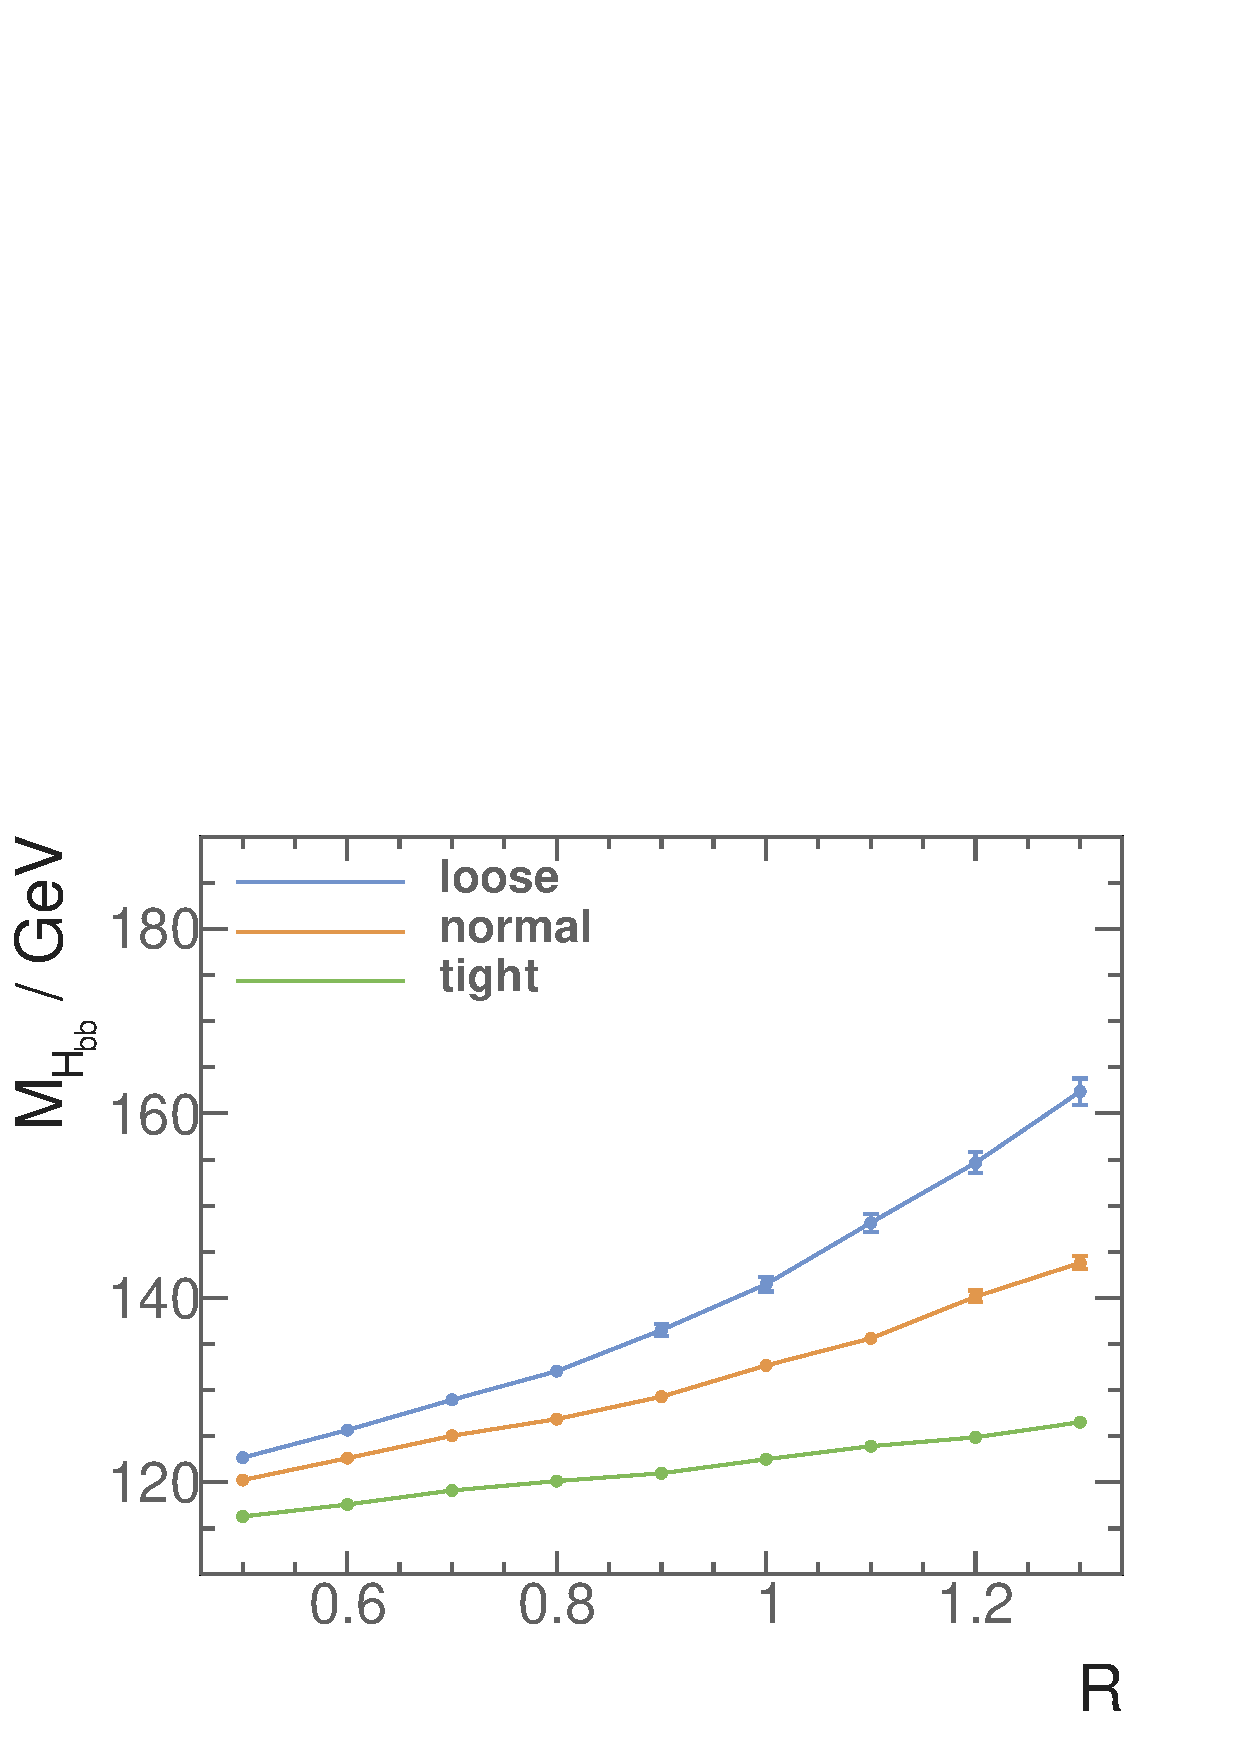
\includegraphics[width=\textwidth]{{doubleHiggs/resolution/ILD_3TeV_Higgs1_M_R}.pdf}
    \caption{}
    \label{fig:doubleHiggs3Higgs1M}
  \end{subfigure}
  \begin{subfigure}[b]{0.45\textwidth}
    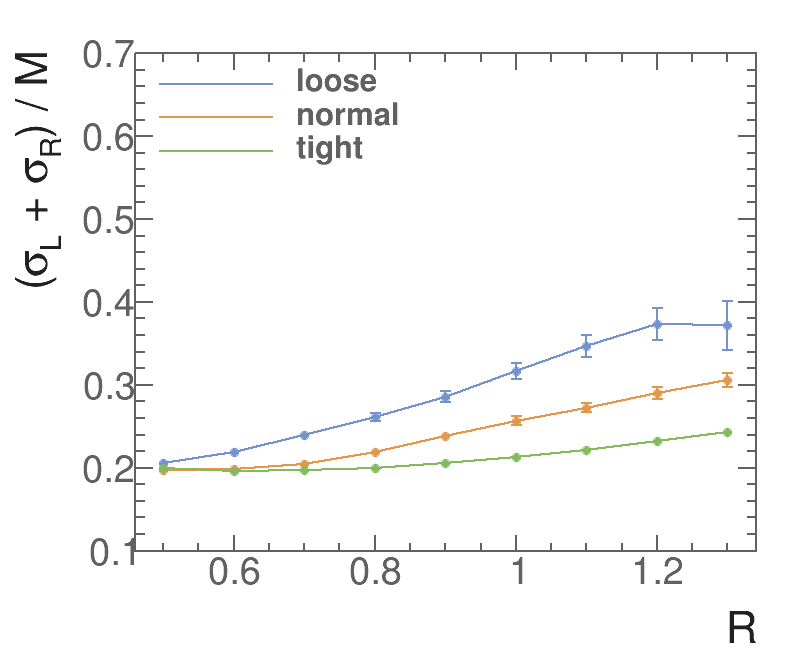
\includegraphics[width=\textwidth]{{doubleHiggs/resolution/ILD_3TeV_Higgs1_SigmaL_add_SigmaR_divide_M_testR}.pdf}
    \caption{}
    \label{fig:doubleHiggs3Higgs1Sigma}
  \end{subfigure}
  \begin{subfigure}[b]{0.45\textwidth}
    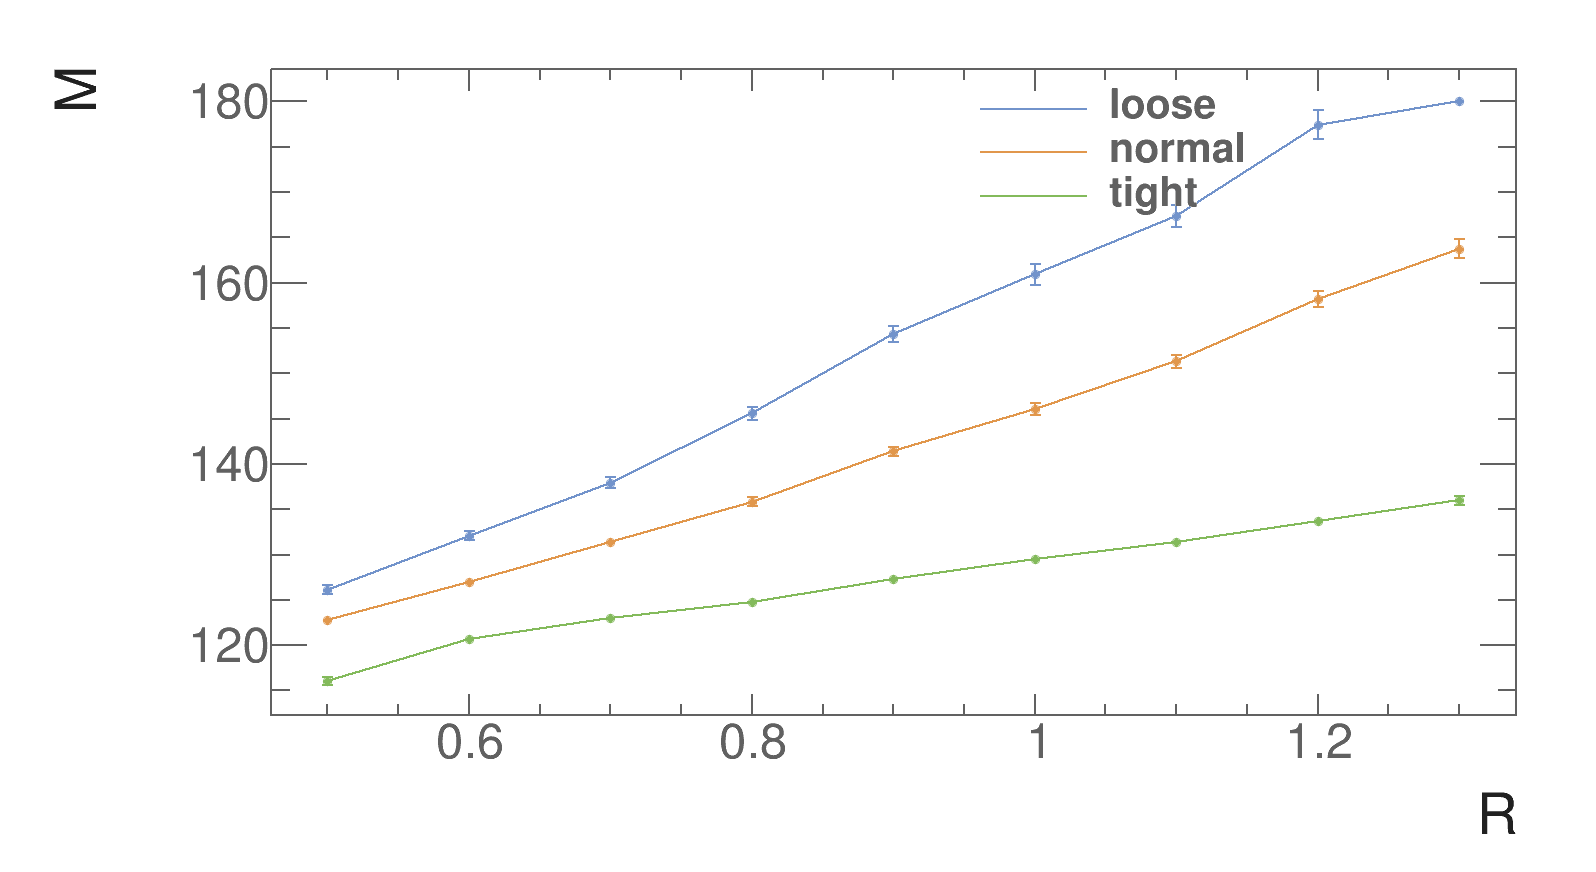
\includegraphics[width=\textwidth]{{doubleHiggs/resolution/ILD_3TeV_Higgs2_M_R}.pdf}
    \caption{}
    \label{fig:doubleHiggs3Higgs2M}
  \end{subfigure}
  \begin{subfigure}[b]{0.45\textwidth}
    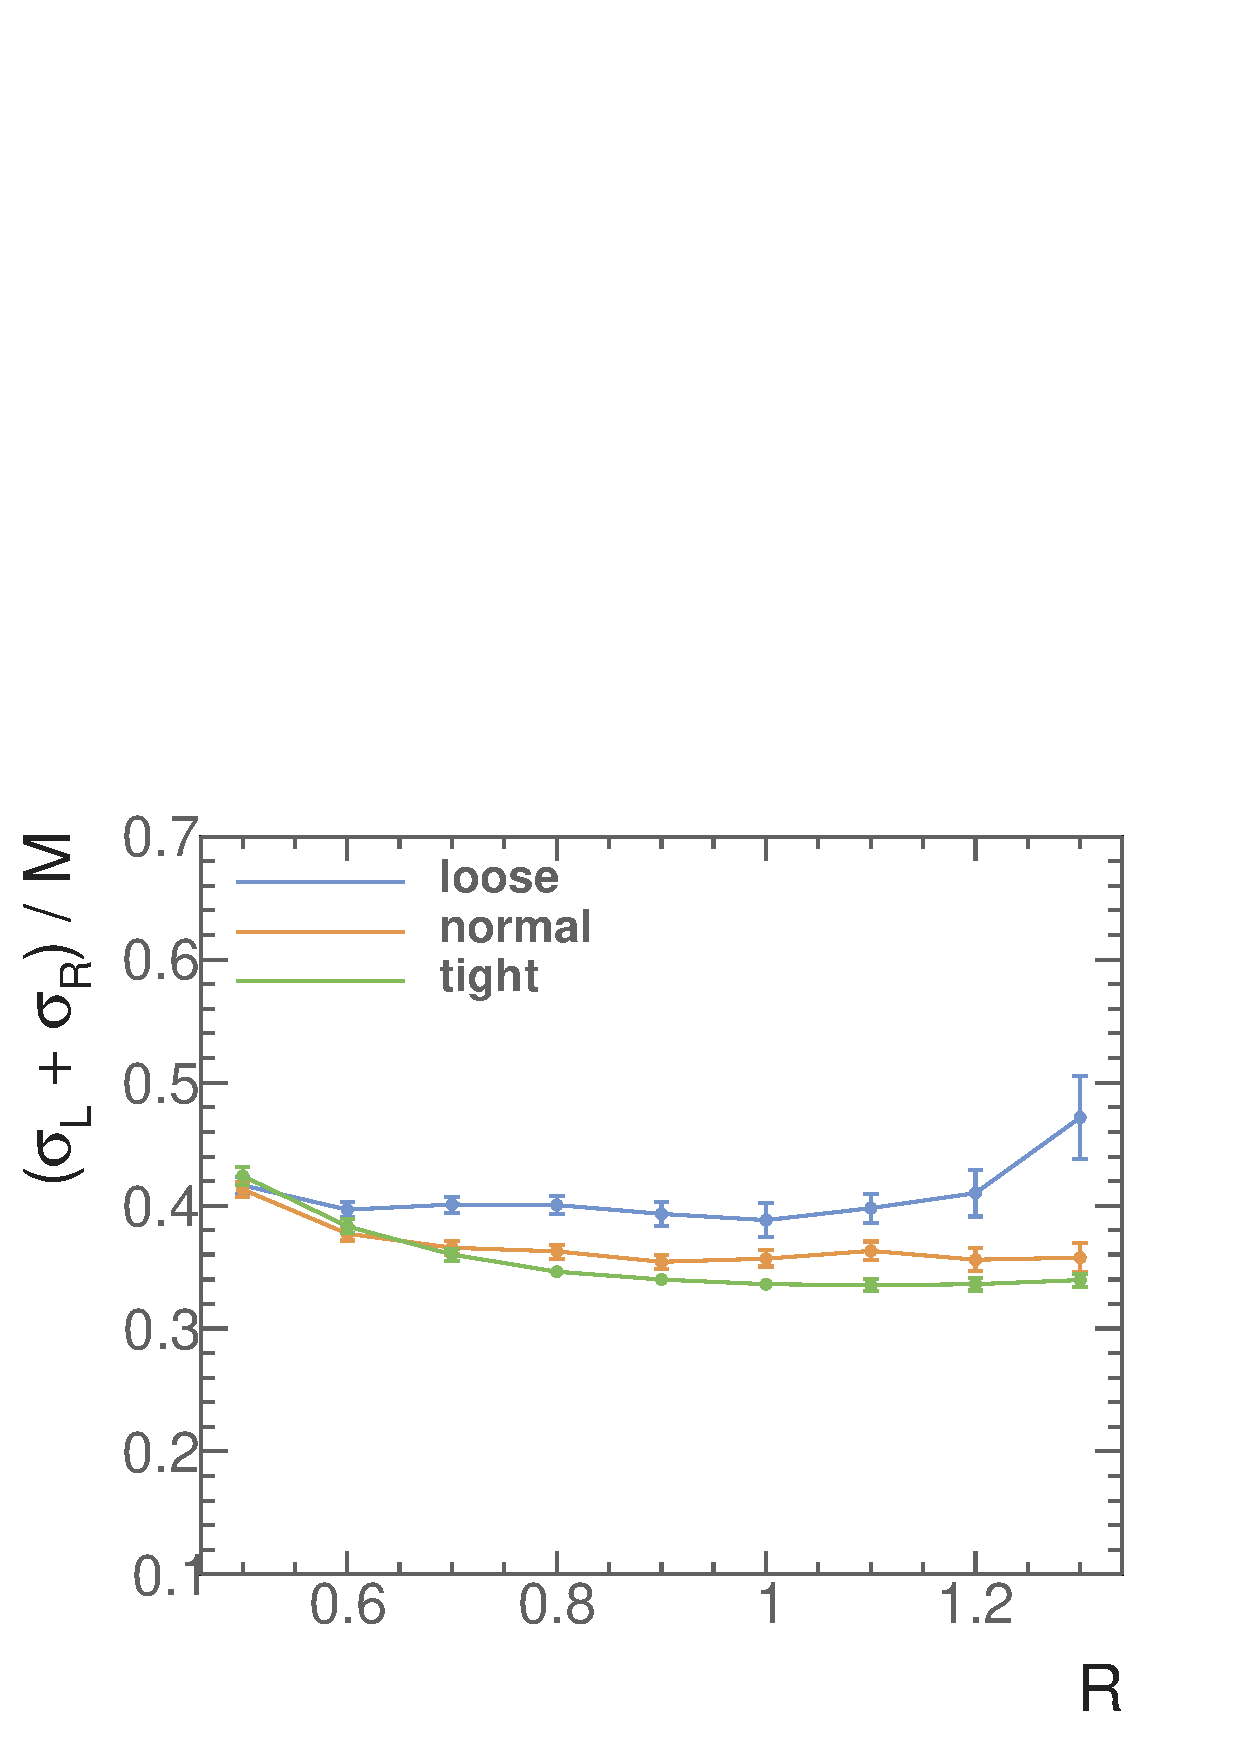
\includegraphics[width=\textwidth]{{doubleHiggs/resolution/ILD_3TeV_Higgs2_SigmaL_add_SigmaR_divide_M_testR}.pdf}
    \caption{}
    \label{fig:doubleHiggs3Higgs2Sigma}
  \end{subfigure}
  \begin{subfigure}[b]{0.45\textwidth}
    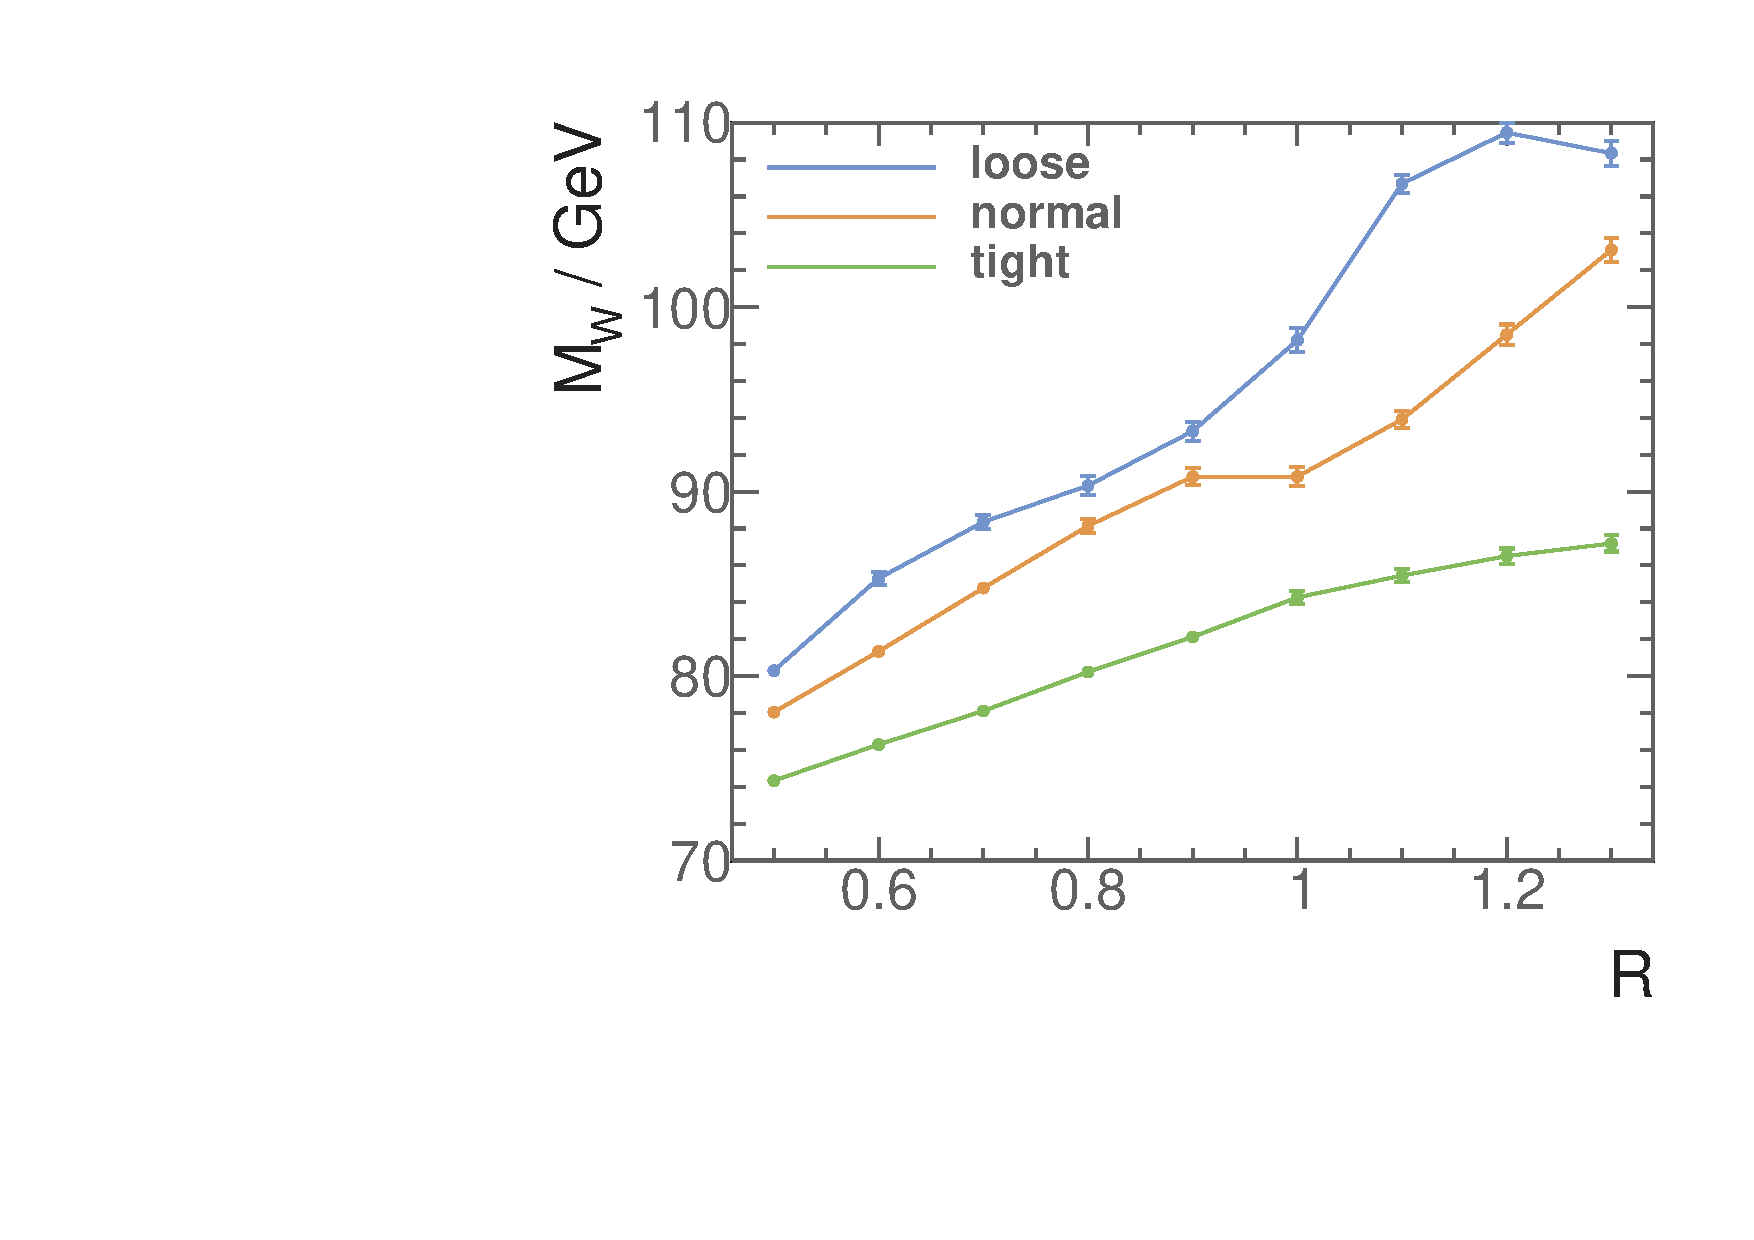
\includegraphics[width=\textwidth]{{doubleHiggs/resolution/ILD_3TeV_W_M_testR}.pdf}
    \caption{}
    \label{fig:doubleHiggs3WM}
  \end{subfigure}
  \begin{subfigure}[b]{0.45\textwidth}
    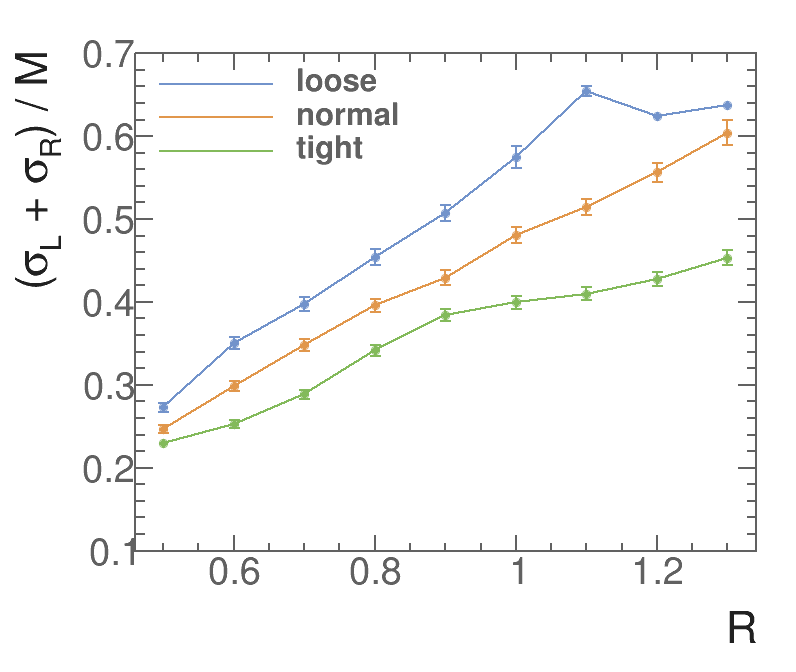
\includegraphics[width=\textwidth]{{doubleHiggs/resolution/ILD_3TeV_W_SigmaL_add_SigmaR_divide_M_testR}.pdf}
    \caption{}
    \label{fig:doubleHiggs3WSigma}
  \end{subfigure}
\caption[Fitted mass peak positions and relative mass resolution of \Hbb, \HWW and \PW at \rootS{3}.]%
   {\FIGURE{fig:doubleHiggs3Higgs1M}, \ref{fig:doubleHiggs3Higgs2M}, and \ref{fig:doubleHiggs3WM}  show fitted mass peak positions of \Hbb, \HWW, and \PW, respectively, for loose, normal and tight selected PFO collection as a function of $R$ at \rootS{3}. \FIGURE{fig:doubleHiggs3Higgs1Sigma}, \ref{fig:doubleHiggs3Higgs2Sigma}, and \ref{fig:doubleHiggs3WSigma} show relative mass resolutions of \Hbb, \HWW, and \PW, respectively, for loose, normal and tight selected \PFO collection as a function of  $R$ at \rootS{3}.}
   \label{fig:doubleHiggs3TeVMassFit}
\end{figure}

\begin{table}[!tbp]
\begin{tabular}{lrr}
\hline
\hline
Jet Parameters  & \rootS{3}  \\
\hline
$\mu_{\Hbb}$  & $119.1_{\pm0.3}$  \\
$\sigma_{L,\Hbb}$ & $15.0_{\pm0.3}$  \\
$\sigma_{R,\Hbb}$ & $8.4_{\pm0.2}$  \\
\hline
$\mu_{\HWW}$ &  $123.0_{\pm0.3}$  \\
$\sigma_{L,\HWW}$ & $36.6_{\pm0.6}$  \\
$\sigma_{R,\HWW}$ & $7.4_{\pm0.2}$  \\
\hline
$\mu_{\PW}$  & $78.1_{\pm0.3}$ \\
$\sigma_{L,\PW}$ & $13.1_{\pm0.4}$  \\
$\sigma_{R,\PW}$ &  $9.5_{\pm0.2}$  \\
\hline
\hline
\end{tabular}
\caption
[The extracted fitted parameters of optimal jet reconstructions at \rootS{3}.] %
{The extracted fitted parameters of optimal jet reconstructions for \tightPFO with $R = 0.7$ at \rootS{3}.}
\label{tab:doubleHiggs3TeVFitParameters}
\end{table}

The flavour tagging processor is trained with the optimal jet parameters at \rootS{3}. The performance of the flavour tagging  with training samples is shown in \Figure{fig:doubleHiggsBtag3TeV}. Comparing this to the performance at \rootS{1.4}, the performance is slightly worse, because at high \sqrtS, particles at more collimated and more difficult to separate.
%high energy or high energies?

\begin{figure}[!htbp]
    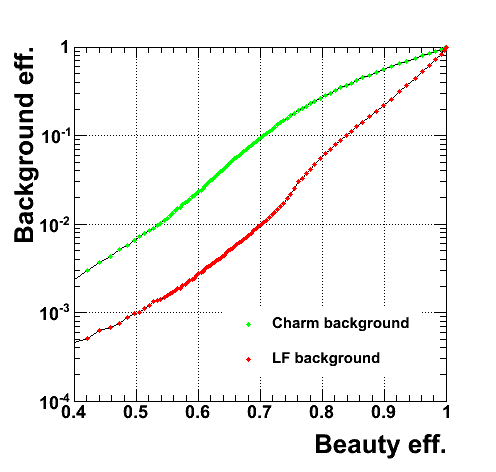
\includegraphics[width=0.45\textwidth]{{doubleHiggs/eval-lcfiweights_tR0_7_3000_2jets-test}.pdf}
    \caption
   {Performance of b-jet tagging with training samples at \rootS{3}.}
   \label{fig:doubleHiggsBtag3TeV}
\end{figure}

%why have the pre-selection cuts changed?
The pre-selection cuts at \rootS{3} are largely the same as ones for \rootS{1.4} analysis. The cuts are listed in \Table{tab:doubleHiggs3TeVPreSel}. The reason for using a different b-jet tag cut is because the performance of flavour tagging is worse at high \sqrtS. \FIGURE{fig:doubleHiggs3PreSelbtag} shows the distribution of the highest b-jet tag, where the cut above 0.7 helps to reduce background events with no b-jet in final states.  \FIGURE{fig:doubleHiggs3PreSelmHH} shows the distribution of the invariant mass of the two Higgs system, where the cut above 150\,GeV is effective against samples with two quark final states.

%The cut is aggressive to compensate for the worse performance of the flavour tagging at high \sqrtS.



\begin{table}[!htbp]
\begin{tabular}{lr}
\hline
\hline
Pre-selection  &  \rootS{3}  \\
\hline
Discriminative pre-selection & \multicolumn{1}{R{0.5\textwidth}}{$m_{\HH} > 150\,GeV$, $B_1 > 0.7$,  $\pT_{\HH} > 30\,GeV$} \\
Loose cuts for MVA &  \multicolumn{1}{R{0.5\textwidth}}{$m_{\Hbb} < 500\,GeV$, $m_{\HWW} < 800\,GeV$, $m_{\PW} < 200\,GeV$, $m_{\HH} <3000\,GeV$} \\
Mutually exclusive & \sumBtag{4} < 2.3, \y{34} < 3.6 \\
\hline
\hline
\end{tabular}
\caption
{Pre-selection cuts at \rootS{3}.}
\label{tab:doubleHiggs3TeVPreSel}
\end{table}

\begin{figure}[!tbp]
  \begin{subfigure}[b]{0.45\textwidth}
    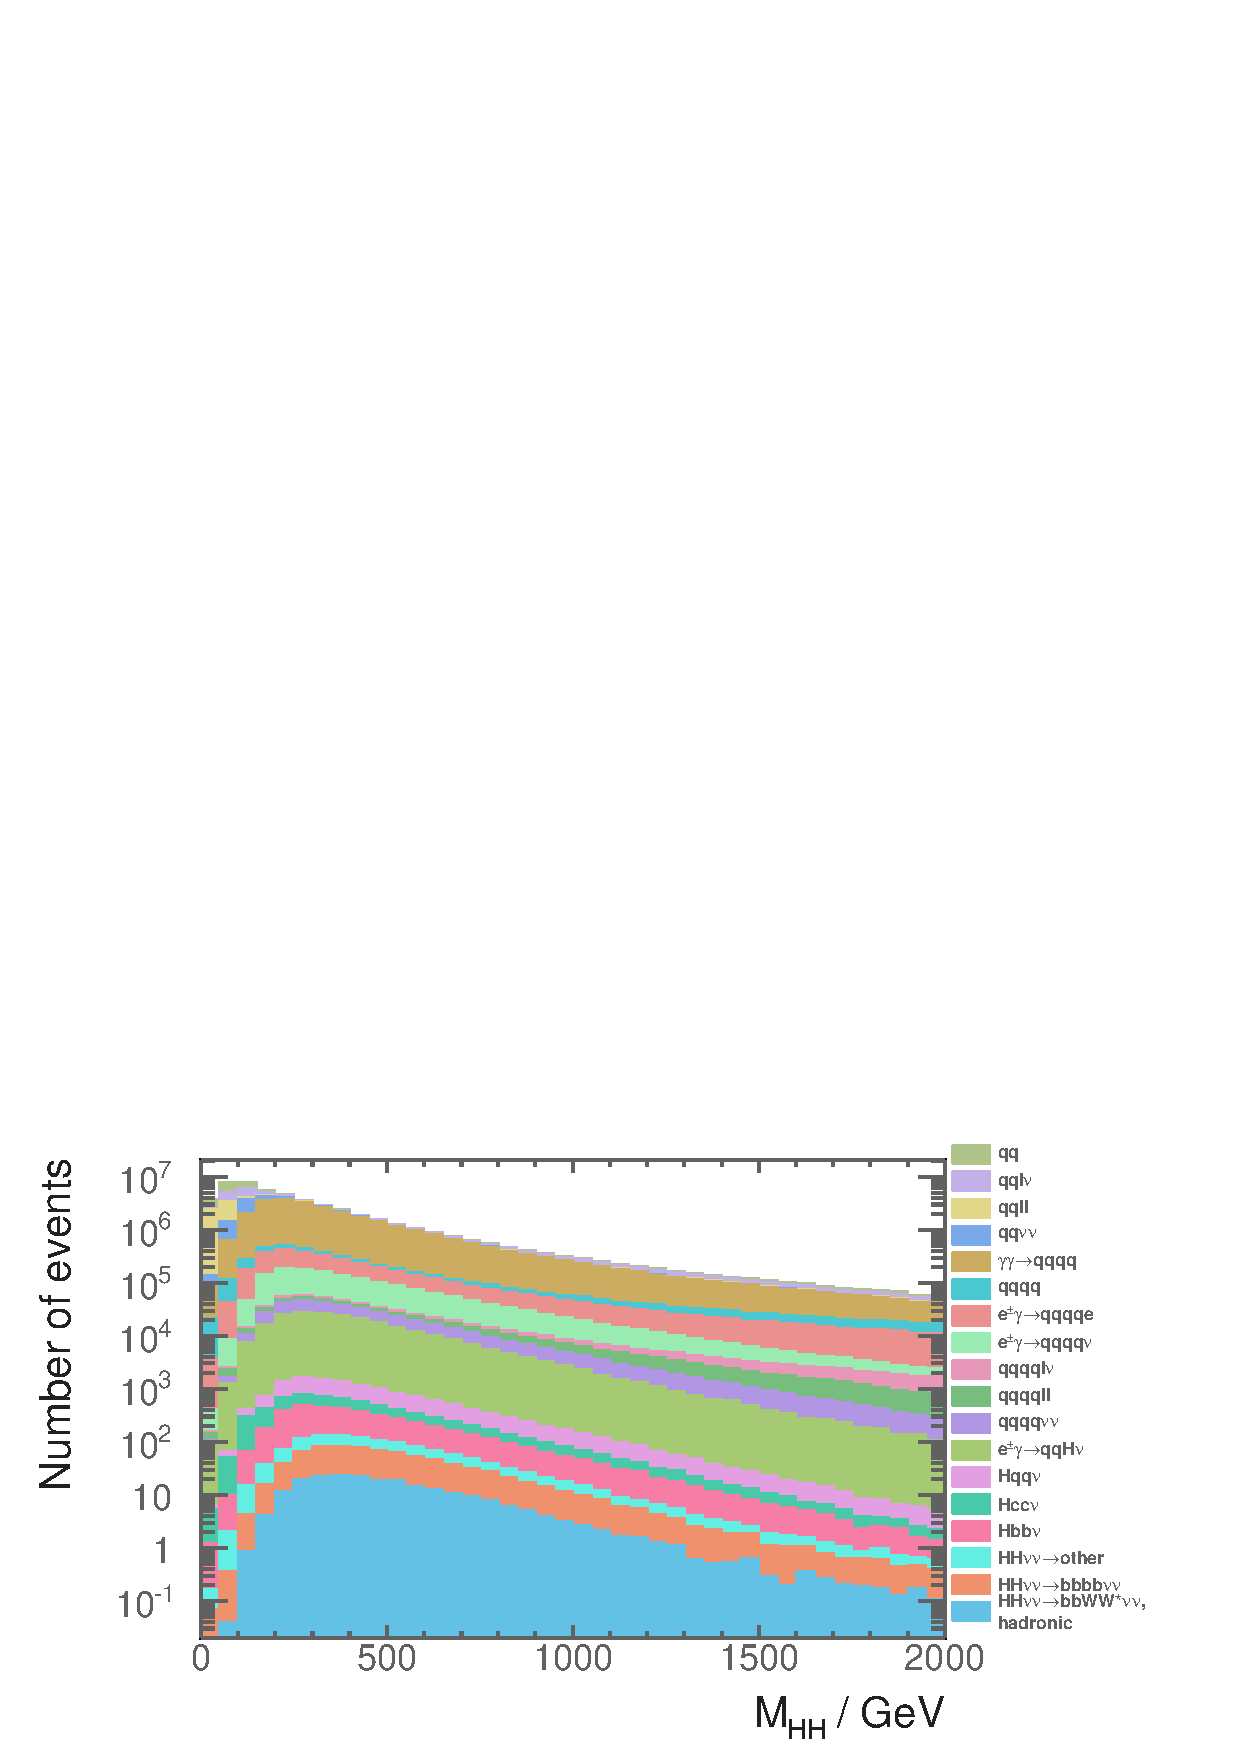
\includegraphics[width=\textwidth]{{doubleHiggs/preSel/tR0_7_6jet_btag2_Higgs_all_M_TMVA201612083TeVtR0_7_qq_btag2_prepare}.pdf}
    \caption{}
    \label{fig:doubleHiggs3PreSelmHH}
  \end{subfigure}
    \begin{subfigure}[b]{0.45\textwidth}
    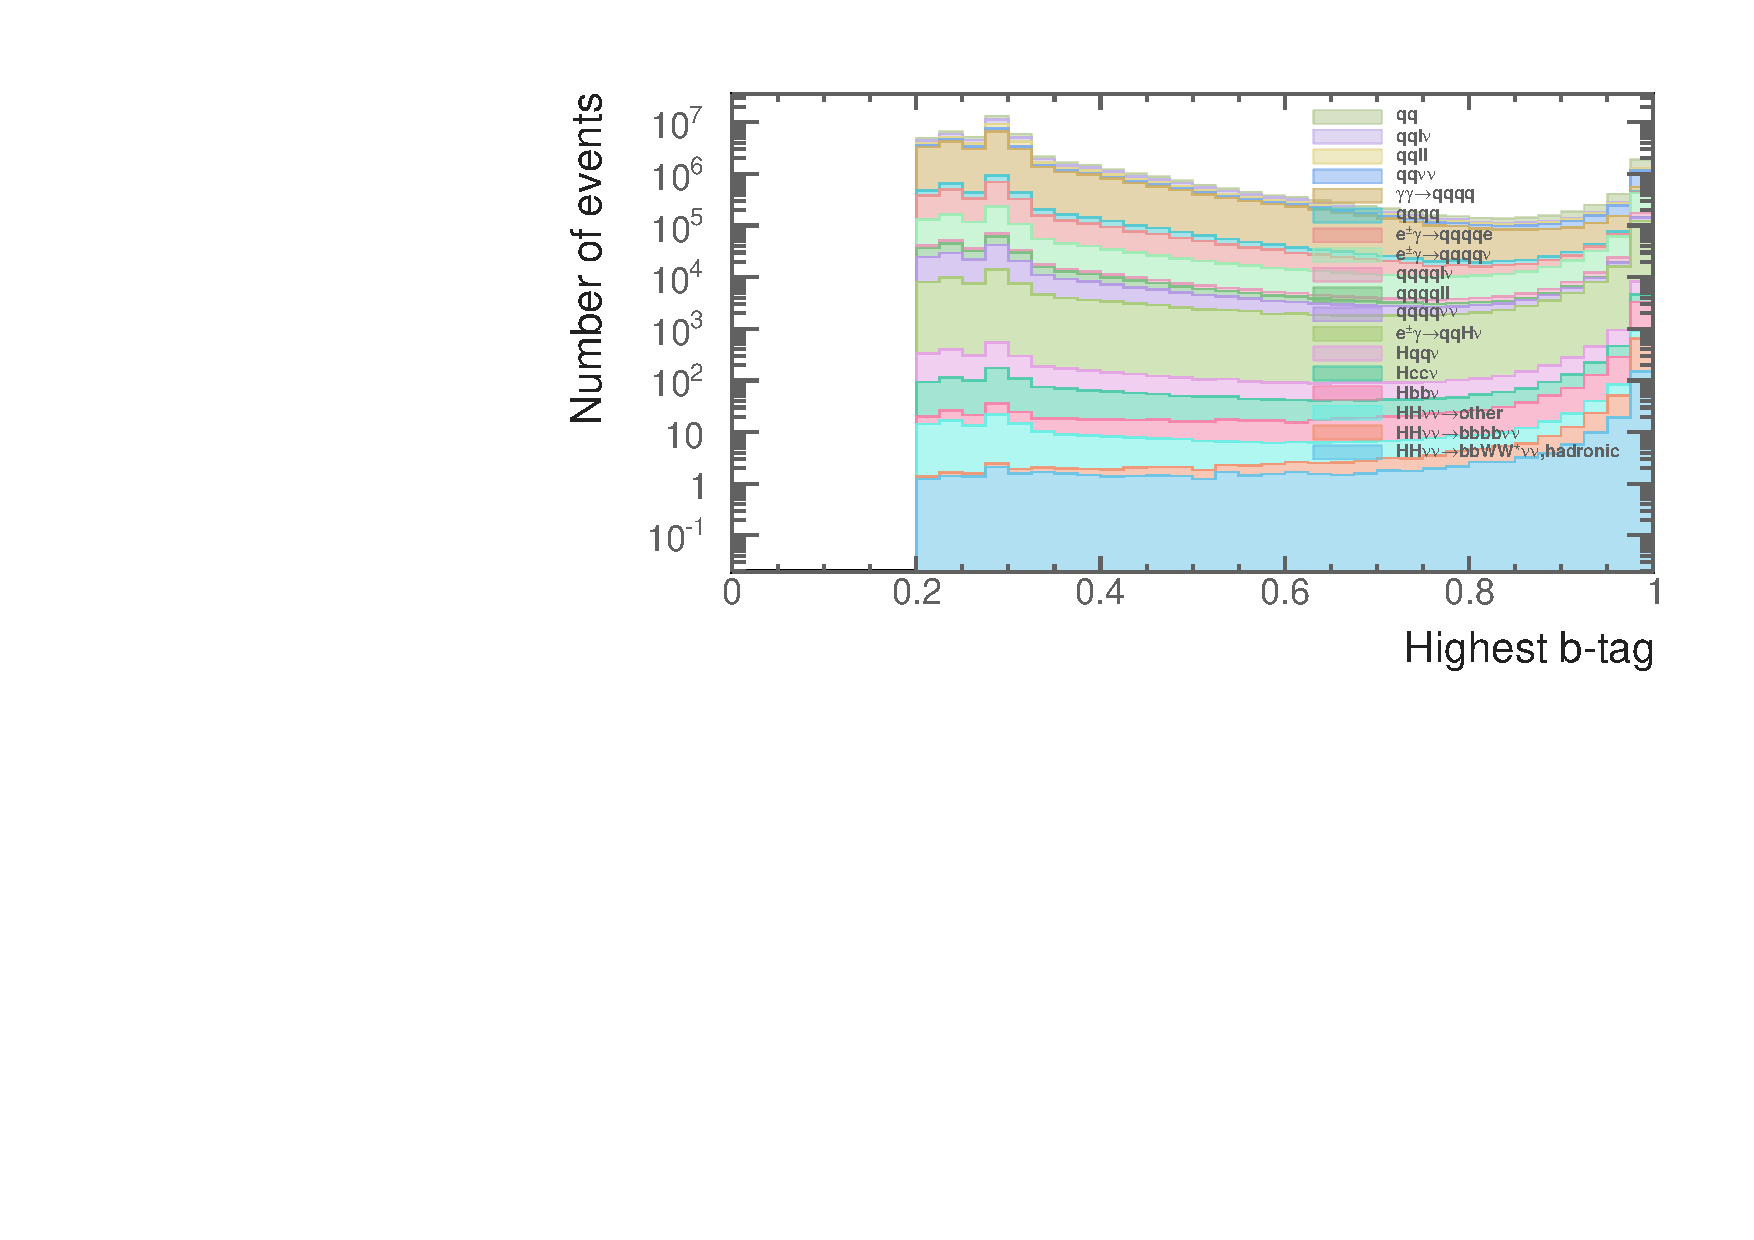
\includegraphics[width=\textwidth]{{doubleHiggs/preSel/tR0_7_6jet_btag2_bTag1_TMVA201612083TeVtR0_7_qq_btag2_prepare}.pdf}
    \caption{}
    \label{fig:doubleHiggs3PreSelbtag}
  \end{subfigure}
\caption[Distributions of variables used  in discriminative pre-selection cuts at \rootS{3}.]%
   {Distributions of variables used  in discriminative pre-selection cuts at \rootS{3}, after rejecting events with identified leptons and jet pairing.}
   \label{fig:doubleHiggs3TeVPreSelection}
\end{figure}

% The cut on $m_{HH}$ is effective against background with fewer number of quarks in the final states. The cut on $B_1$ is effective against final states with no b quark.


\begin{table}[!tbp]\centering
% TODO fix lumi correction for e gamma, gamma e
% TODO change some of sample cross section for  electron-photon interaction with four quarks and a neutrino final state
%\small{
\small
\begin{tabular}{lrrrr}
\hline \hline
 \multicolumn{1}{m{3.5cm}}{Channel / Efficiency \rootS{3}} &  \multicolumn{1}{m{2cm}}{Expected number of events}  & \multicolumn{1}{m{2cm}}{Lepton ID and jet pairing} & \multicolumn{1}{m{1.5cm}}{$m_{HH}>150\xspace{GeV}$} & \multicolumn{1}{m{1.5cm}}{$B_{1}>0.7$} \\
\hline
\eeToHH $\to$ \\
\HepProcess{ \Pbottom \APbottom \PWplus \PWminus \Pnue \APnue}, hadronic             &146.0& 80.2\% & 79.9\% & 69.7\%\\
\hline
\eeToHH $\to$ \\
\HepProcess{ \Pbottom \APbottom \Pbottom \APbottom \Pnue \APnue}             &355.0& 83.4\% & 82.9\% & 81.2\% \\
\eeToHH $\to$ other & 675.0 & 36.7\% & 35.8\% & 25.2\% \\
\hline
\eeTo{\qlight \qlight \PHiggs \Pnu \APnu}  & 6115.4 & 59.5\% & 58.5\% & 40.4\%\\
\eeTo{\Pcharm \APcharm \PHiggs \Pnu \APnu}  & 2249.9 & 64.8\%& 58.4\%& 39.3\%\\
\eeTo{\Pbottom \APbottom \PHiggs \Pnu \APnu}  & 2197.7 & 69.7\%& 68.4\%& 64.2\%\\

\eeTo{ \Pquark \Pquark \Pquark \Pquark}   &   1093000.0& 48.5\% & 39.7\%& 3.0\%\\
\eeTo{ \Pquark \Pquark \Pquark \Pquark \Plepton \Plepton}& 338600.0 & 14.7\%& 14.2\%& 0.7\%\\
\eeTo{ \Pquark \Pquark \Pquark \Pquark \Plepton \Pnu}& 213200.0 & 19.7\%& 19.4\%& 10.0\%\\
\eeTo{ \Pquark \Pquark \Pquark \Pquark \Pnu \APnu} & 143000.0& 58.4\%& 57.3\%& 11.9\%\\

\eeTo{ \Pquark \Pquark} &  5897800.0 & 62.8\%& 13.2\%& 2.7\%\\
\eeTo{ \Pquark \Pquark \Plepton \Pnu} &  11121800 & 28.3\%& 11.9\%& 0.3\%\\
\eeTo{ \Pquark \Pquark \Pl \Pl} &  6639200.0 & 38.3\%& 2.9\%& 0.7\%\\
\eeTo{ \Pquark \Pquark \Pnu \Pnu} & 2635000.0 & 71.4\%& 24.1\%& 5.3\% \\
\hline
\egamma{\Pepm}{\Pphoton}{BS}{\Pepm \Pquark \Pquark \Pquark \Pquark} & 4006722.2  & 23.3\%& 21.5\%& 0.8\%\\
%\egamma{\Pem}{\Pphoton}{BS}{\Pem \Pquark \Pquark \Pquark \Pquark} & 2004388.1  & 23.3\%& 21.5\%& 0.8\%\\
%\egamma{\Pep}{\Pphoton}{BS}{\Pep \Pquark \Pquark \Pquark \Pquark} & 2002334.1 & 23.4\%& 21.6\%& 0.8\%\\
\egamma{\Pepm}{\Pphoton}{EPA}{\Pepm \Pquark \Pquark \Pquark \Pquark} & 1151200.0& 12.0\%& 11.0\%& 0.5\%\\
%\egamma{\Pem}{\Pphoton}{EPA}{\Pem \Pquark \Pquark \Pquark \Pquark} & 575600.0& 12.0\%& 11.0\%& 0.5\%\\
%\egamma{\Pep}{\Pphoton}{EPA}{\Pep \Pquark \Pquark \Pquark \Pquark}  & 575600.0 & 12.0\% & 10.9\%& 0.4\%\\
\egamma{\Pepm}{\Pphoton}{BS}{\Pnu \Pquark \Pquark \Pquark \Pquark}& 829184.0  & 61.5\%& 59.3\%& 19.9\%\\
%\egamma{\Pem}{\Pphoton}{BS}{\Pnu \Pquark \Pquark \Pquark \Pquark}& 414750.0  & 61.7\%& 59.5\%& 20.4\%\\
%\egamma{\Pep}{\Pphoton}{BS}{\APnu \Pquark \Pquark \Pquark \Pquark}& 414434.0 & 61.2\% & 59.1\%& 19.4\%\\
\egamma{\Pepm}{\Pphoton}{EPA}{\Pnu \Pquark \Pquark \Pquark \Pquark}& 216800.0  & 30.8\% & 29.8\%& 9.4\%\\
%\egamma{\Pem}{\Pphoton}{EPA}{\Pnu \Pquark \Pquark \Pquark \Pquark}& 108400.0  & 30.9\% & 29.9\%& 9.6\%\\
%\egamma{\Pep}{\Pphoton}{EPA}{\APnu \Pquark \Pquark \Pquark \Pquark}& 108400.0  & 30.7\%& 29.7\%& 9.1\% \\
\egamma{\Pepm}{\Pphoton}{BS}{\Pquark \Pquark \PHiggs \Pnu} & 185018.0  & 58.2\% &56.1\%& 37.2\% \\
%\egamma{\Pem}{\Pphoton}{BS}{\Pquark \Pquark \PHiggs \Pnu} & 92588.0  & 58.3\% &56.2\%& 37.3\% \\
%\egamma{\Pep}{\Pphoton}{BS}{\Pquark \Pquark \PHiggs \Pnu} & 92430.0 & 58.1\% & 56.0\% & 37.1\% \\
\egamma{\Pepm}{\Pphoton}{EPA}{\Pquark \Pquark \PHiggs \Pnu} & 46800.0 & 29.9\% &28.9\% & 19.1\% \\
%\egamma{\Pem}{\Pphoton}{EPA}{\Pquark \Pquark \PHiggs \Pnu} & 23400.0 & 30.1\% &29.2\% & 19.4\% \\
%\egamma{\Pep}{\Pphoton}{EPA}{\Pquark \Pquark \PHiggs \Pnu} & 23400.0   & 29.7\% & 28.6\% & 18.8\% \\
\hline
\gammagamma{\Pphoton}{BS}{\Pphoton}{BS}{ \Pquark \Pquark \Pquark \Pquark}& 18009413.9  & 54.2\%& 49.2\%& 1.9\%\\
\gammagamma{\Pphoton}{BS}{\Pphoton}{EPA}{ \Pquark \Pquark \Pquark \Pquark}& 3824548.1  &33.5\%& 30.2\%& 1.2\%\\
\gammagamma{\Pphoton}{EPA}{\Pphoton}{BS}{ \Pquark \Pquark \Pquark \Pquark}& 3828498.1 & 33.7\%& 30.3\%& 1.2\%\\
\gammagamma{\Pphoton}{EPA}{\Pphoton}{EPA}{ \Pquark \Pquark \Pquark \Pquark}& 805400.0 & 22.0\% & 19.8\% & 0.8\%\\
\hline \hline
\end{tabular}

\caption[Signal and background events with selection efficiency and event numbers after the pre-selection cuts at \rootS{3}]%
{List of signal and background samples with selection efficiencies and event numbers after the pre-selection cuts  at \rootS{3}, assuming a luminosity of 2000$fb^{-1}$. The selection efficiencies are presented in a ``flow'' fashion. Every selection cut contains all the cuts to the left of it.
}
\label{tab:doubleHiggs3TeVPreslection}
\end{table}

The cutsto aid the MVA at \rootS{3} are largely the same as the ones at \rootS{3}, apart from the difference on the cut of the invariant mass of \HH due to higher \sqrtS. The selection efficiency of the lepton veto and the pre-selection is shown in \Table{tab:doubleHiggs3TeVPreslection}.

The mutually exclusive cuts divide samples - both signal and background - into two mutually exclusive sets for the parallel analyses of  two subchannels; \eeToHHbbWWHad and \eeToHHbbbb. The cuts are obtained using the same strategy in \Section{sec:doubleHiggsMutualExclusive}. The cuts and efficiencies are listed in \Table{tab:doubleHiggs3TeVPreSel}. The two dimensional spaces for two sub-channels are shown in \Figure{fig:doubleHiggs3TeVMutualPreselection}. The selection efficiencies after the mutually exclusive cuts are shown in \Table{tab:doubleHiggs3TeVPreslectionPart2}.



\begin{figure}[!tbp]
  \begin{subfigure}[b]{0.45\textwidth}
    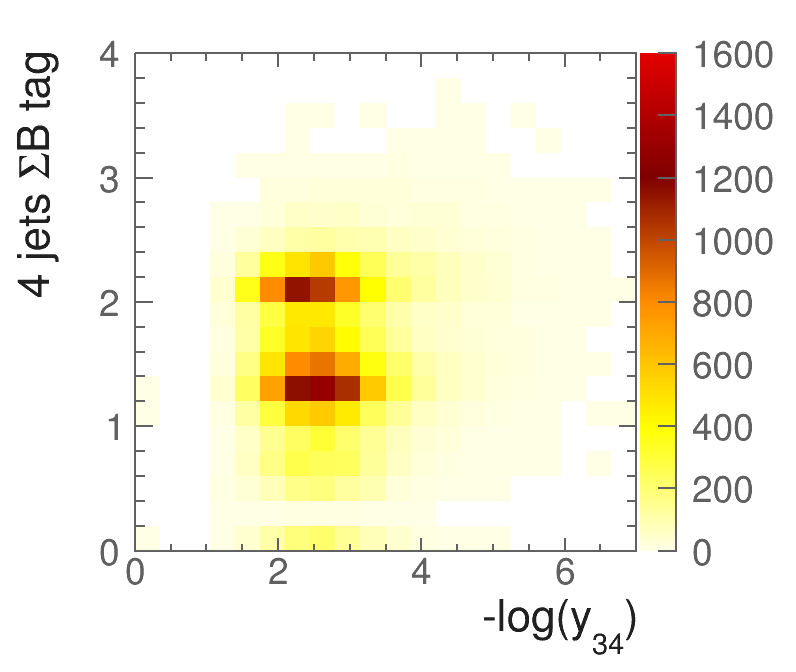
\includegraphics[width=\textwidth]{{doubleHiggs/mutual6025bbWW}.pdf}
    \caption{\eeToHHbbWW, hadronic}
    \label{fig:doubleHiggs3MutualbbWW}
  \end{subfigure}
    \begin{subfigure}[b]{0.45\textwidth}
    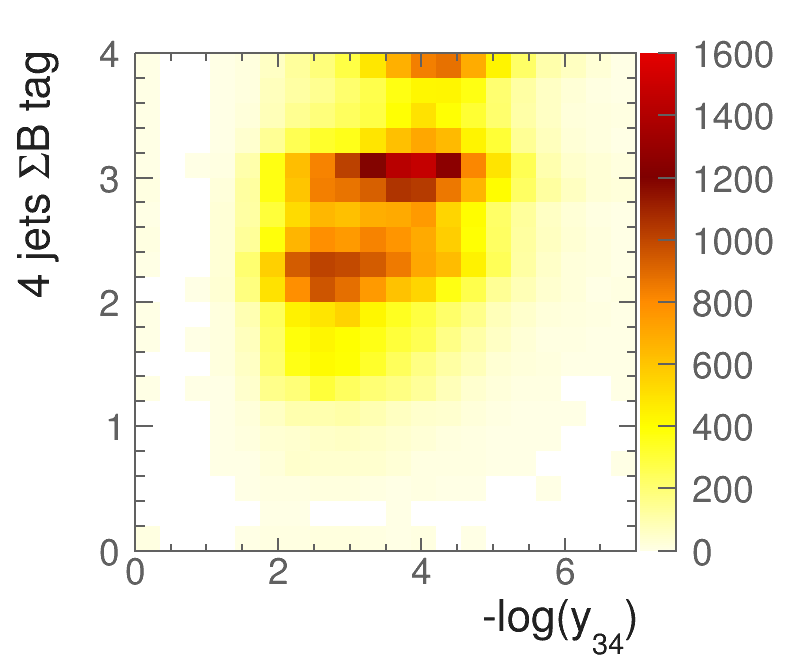
\includegraphics[width=\textwidth]{{doubleHiggs/mutual6025bbbb}.pdf}
    \caption{\eeToHHbbbb}
    \label{fig:doubleHiggs3Mutualbbbb}
  \end{subfigure}
\caption[Sum of b-jet tag as a function of \y{34} at \rootS{3}]%
   {Sum of b-jet tag as a function of \y{34} at \rootS{3}, shown for hadronic decay of \eeToHHbbWWHad and \eeToHHbbWW sub-channels. }
   \label{fig:doubleHiggs3TeVMutualPreselection}
\end{figure}

\begin{comment}
\begin{table}\centering
\begin{tabular}{llrr}
\hline
\hline
\sqrtS & $selection$ & \multicolumn{1}{m{4cm}}{\eeToHHbbqqqq Selection Efficiency} & \multicolumn{1}{m{4cm}}{\eeToHHbbbb Selection Efficiency} \\
1.4\,TeV &  \sumBtag{4} < 2.3 and \y{34} < 3.7 & 86\% & 78\% \\
3\,TeV &  \sumBtag{4} < 2.3 and \y{34} < 3.6 & 89\% & 82\% \\
\hline
\hline
\end{tabular}
\caption[Mutually exclusive cuts] %
{Mutually exclusive cuts, for full signal samples}
\label{tab:doubleHiggsMutualCuts}
\end{table}
\end{comment}

\begin{table}[!tbp]\centering
\small
\begin{tabular}{lrrrr}
\hline \hline
 \multicolumn{1}{L{0.3\textwidth}}{Channel} &  \multicolumn{1}{R{0.3\textwidth}}{Previous cuts and loose cuts}  & \multicolumn{1}{R{0.3\textwidth}}{Mutually exclusive} \\
\hline
\eeToHH $\to$ \\
\HepProcess{ \Pbottom \APbottom \PWplus \PWminus \Pnue \APnue}, hadronic             & 69.5\% & 61.7\%\\
\hline
\eeToHH $\to$ \\
\HepProcess{ \Pbottom \APbottom \Pbottom \APbottom \Pnue \APnue}             & 81.1\% & 18.8\% \\
\eeToHH $\to$ other & 25.1\% & 20.0\% \\
\hline
\eeTo{\qlight \qlight \PHiggs \Pnu \APnu}   & 40.3\% & 35.9\%\\
\eeTo{\Pcharm \APcharm \PHiggs \Pnu \APnu} & 39.2\%& 26.2\%\\
\eeTo{\Pbottom \APbottom \PHiggs \Pnu \APnu} & 64.2\%& 25.9\%\\

\eeTo{ \Pquark \Pquark \Pquark \Pquark}   & 2.5\%& 1.4\%\\
\eeTo{ \Pquark \Pquark \Pquark \Pquark \Plepton \Plepton} & 0.7\%& 0.6\%\\
\eeTo{ \Pquark \Pquark \Pquark \Pquark \Plepton \Pnu} & 9.2\%& 7.2\%\\
\eeTo{ \Pquark \Pquark \Pquark \Pquark \Pnu \APnu} & 11.8\%& 9.0\%\\

\eeTo{ \Pquark \Pquark} & 2.5\%& 1.4\%\\
\eeTo{ \Pquark \Pquark \Plepton \Pnu} & 0.3\%& 0.1\%\\
\eeTo{ \Pquark \Pquark \Pl \Pl} & 0.7\%& 0.4\%\\
\eeTo{ \Pquark \Pquark \Pnu \Pnu} & 5.3\%& 3.1\% \\
\hline
\egamma{\Pepm}{\Pphoton}{BS}{\Pepm \Pquark \Pquark \Pquark \Pquark}& 0.8\%& 0.7\%\\
%\egamma{\Pem}{\Pphoton}{BS}{\Pem \Pquark \Pquark \Pquark \Pquark}& 0.8\%& 0.7\%\\
%\egamma{\Pep}{\Pphoton}{BS}{\Pep \Pquark \Pquark \Pquark \Pquark} & 0.8\%& 0.7\%\\
\egamma{\Pepm}{\Pphoton}{EPA}{\Pepm \Pquark \Pquark \Pquark \Pquark} & 0.4\%& 0.4\%\\
%\egamma{\Pem}{\Pphoton}{EPA}{\Pem \Pquark \Pquark \Pquark \Pquark} & 0.4\%& 0.4\%\\
%\egamma{\Pep}{\Pphoton}{EPA}{\Pep \Pquark \Pquark \Pquark \Pquark}   & 0.4\%& 0.3\%\\
\egamma{\Pepm}{\Pphoton}{BS}{\Pnu \Pquark \Pquark \Pquark \Pquark} & 19.8\%& 16.4\%\\
%\egamma{\Pem}{\Pphoton}{BS}{\Pnu \Pquark \Pquark \Pquark \Pquark} & 20.3\%& 16.8\%\\
%\egamma{\Pep}{\Pphoton}{BS}{\APnu \Pquark \Pquark \Pquark \Pquark} & 19.3\%& 15.9\%\\
\egamma{\Pepm}{\Pphoton}{EPA}{\Pnu \Pquark \Pquark \Pquark \Pquark} & 9.2\%& 7.6\%\\
%\egamma{\Pem}{\Pphoton}{EPA}{\Pnu \Pquark \Pquark \Pquark \Pquark} & 9.4\%& 7.8\%\\
%\egamma{\Pep}{\Pphoton}{EPA}{\APnu \Pquark \Pquark \Pquark \Pquark}& 8.9\%& 7.3\% \\
\egamma{\Pepm}{\Pphoton}{BS}{\Pquark \Pquark \PHiggs \Pnu} &37.2\%& 30.2\% \\
%\egamma{\Pem}{\Pphoton}{BS}{\Pquark \Pquark \PHiggs \Pnu} &37.2\%& 30.2\% \\
%\egamma{\Pep}{\Pphoton}{BS}{\Pquark \Pquark \PHiggs \Pnu} & 37.1\% & 30.2\% \\
\egamma{\Pem}{\Pphoton}{EPA}{\Pquark \Pquark \PHiggs \Pnu} & 18.7\% & 15.5\% \\
%\egamma{\Pem}{\Pphoton}{EPA}{\Pquark \Pquark \PHiggs \Pnu} & 19.0\% & 15.7\% \\
%\egamma{\Pep}{\Pphoton}{EPA}{\Pquark \Pquark \PHiggs \Pnu} & 18.4\% & 15.2\% \\
\hline
\gammagamma{\Pphoton}{BS}{\Pphoton}{BS}{ \Pquark \Pquark \Pquark \Pquark}& 1.9\%& 1.7\%\\
\gammagamma{\Pphoton}{BS}{\Pphoton}{EPA}{ \Pquark \Pquark \Pquark \Pquark}& 1.1\%& 1.0\%\\
\gammagamma{\Pphoton}{EPA}{\Pphoton}{BS}{ \Pquark \Pquark \Pquark \Pquark}& 1.1\%& 1.0\%\\
\gammagamma{\Pphoton}{EPA}{\Pphoton}{EPA}{ \Pquark \Pquark \Pquark \Pquark} & 0.7\% & 0.6\%\\
\hline \hline
\end{tabular}
\caption[List of signal and background samples after loose cuts and mutually exclusive cuts at \rootS{3}.]
{List of signal and background samples with the selection efficiencies after loose cuts and mutually exclusive cuts at \rootS{3}. The selection efficiencies are presented in a ``flow'' fashion. Every selection cut contains all the cuts to the left of it.}
\label{tab:doubleHiggs3TeVPreslectionPart2}
\end{table}

The same set of variables for the MVA are used at \rootS{3} as in the analysis at \rootS{1.4}. The Boosted Decision Tree classifier is optimised at \rootS{3}. The efficiencies of the pre-selection cuts and the efficiencies of the MVA selections are listed in \Table{tab:doubleHiggs3TeVMVA}, alongside the number of events after the MVA selection. Background channels that are dominant after the MVA selection are almost identical to those at \rootS{1.4}. Hence see \Section{sec:doubleHiggsSignalSelResult} for discussion.

\begin{table}[!tbp]\centering
%\small{
\small
\begin{tabular}{lrrrr}
\hline \hline
 \multicolumn{1}{m{3.5cm}}{Channel / Efficiency \rootS{3}} &  \multicolumn{1}{m{2cm}}{N}  & \multicolumn{1}{m{2cm}}{$\varepsilon_{presel}$} & \multicolumn{1}{m{2cm}}{$\varepsilon_{MVA}$} & \multicolumn{1}{m{2cm}}{$N_{MVA}$} \\

\hline
\eeToHH $\to$ \\
\HepProcess{ \Pbottom \APbottom \PWplus \PWminus \Pnue \APnue}, hadronic             &146.0& 61.7\% & 11.6\% & 9.89\\
\hline
\eeToHH $\to$ \\
\HepProcess{ \Pbottom \APbottom \Pbottom \APbottom \Pnue \APnue}             &355.0& 18.8\% & 1.5\% & 1.05 \\
\eeToHH $\to$ other                             & 675.0 & 20.0\% & 3.6\% & 4.51 \\
\hline
\eeTo{\qlight \qlight \PHiggs \Pnu \APnu}  & 6115.4 & 36.0\% & 0.4\% & 9.42\\
\eeTo{\Pcharm \APcharm \PHiggs \Pnu \APnu}  & 2249.9 & 26.3\%& 0.5\%& 3.13\\
\eeTo{\Pbottom \APbottom \PHiggs \Pnu \APnu}  & 2197.7 & 25.8\%& 1.2\%& 6.82\\

\eeTo{ \Pquark \Pquark \Pquark \Pquark}   &   1093000.0& 1.4\% & 0.01\%& 1.43\\
\eeTo{ \Pquark \Pquark \Pquark \Pquark \Plepton \Plepton}& 338600.0 & 0.6\%&  - & -\\
\eeTo{ \Pquark \Pquark \Pquark \Pquark \Plepton \Pnu}& 213200.0 & 7.3\%& 0.05\%& 8.35\\
\eeTo{ \Pquark \Pquark \Pquark \Pquark \Pnu \APnu} & 143000.0& 9.0\%& 0.05\%& 6.35\\

\eeTo{ \Pquark \Pquark} &  5897800.0 & 1.4\%&  - & - \\
\eeTo{ \Pquark \Pquark \Plepton \Pnu} &  11121800 & 0.1\%& - & - \\
\eeTo{ \Pquark \Pquark \Pl \Pl} &  6639200.0 & 0.4\%& - & - \\
\eeTo{ \Pquark \Pquark \Pnu \Pnu} & 2635000.0 & 3.1\%&  - & - \\
\hline
\egamma{\Pepm}{\Pphoton}{BS}{\Pepm \Pquark \Pquark \Pquark \Pquark} & 4006722.2  & 0.7\%&  - & - \\
%\egamma{\Pem}{\Pphoton}{BS}{\Pem \Pquark \Pquark \Pquark \Pquark} & 2004388.1  & 0.7\%&  - & - \\
%\egamma{\Pep}{\Pphoton}{BS}{\Pep \Pquark \Pquark \Pquark \Pquark} & 2002334.1 & 0.7\%&  - & - \\
\egamma{\Pepm}{\Pphoton}{EPA}{\Pepm \Pquark \Pquark \Pquark \Pquark} & 1151200.0& 0.4\%&  - & - \\
%\egamma{\Pem}{\Pphoton}{EPA}{\Pem \Pquark \Pquark \Pquark \Pquark} & 575600.0& 0.4\%&  - & - \\
%\egamma{\Pep}{\Pphoton}{EPA}{\Pep \Pquark \Pquark \Pquark \Pquark}  & 575600.0 & 0.3\% &  - & - \\
\egamma{\Pepm}{\Pphoton}{BS}{\Pnu \Pquark \Pquark \Pquark \Pquark}& 829184.0  & 16.4\%& 0.04\%& 61.0\\
%\egamma{\Pem}{\Pphoton}{BS}{\Pnu \Pquark \Pquark \Pquark \Pquark}& 414750.0  & 16.8\%& 0.04\%& 30.7\\
%\egamma{\Pep}{\Pphoton}{BS}{\APnu \Pquark \Pquark \Pquark \Pquark}& 414434.0 & 15.9\% & 0.05\%& 30.3\\
\egamma{\Pepm}{\Pphoton}{EPA}{\Pnu \Pquark \Pquark \Pquark \Pquark}& 216800.0  & 7.6\% & 0.04\%& 6.0\\
%\egamma{\Pem}{\Pphoton}{EPA}{\Pnu \Pquark \Pquark \Pquark \Pquark}& 108400.0  & 7.8\% & 0.04\%& 3.37\\
%\egamma{\Pep}{\Pphoton}{EPA}{\APnu \Pquark \Pquark \Pquark \Pquark}& 108400.0  & 7.3\%& 0.03\%& 2.63 \\
\egamma{\Pepm}{\Pphoton}{BS}{\Pquark \Pquark \PHiggs \Pnu} & 185018.0  & 30.2\% & 0.2\%& 121.7 \\
%\egamma{\Pem}{\Pphoton}{BS}{\Pquark \Pquark \PHiggs \Pnu} & 92588.0  & 30.2\% & 0.2\%& 67.5 \\
%\egamma{\Pep}{\Pphoton}{BS}{\Pquark \Pquark \PHiggs \Pnu} & 92430.0 & 30.3\% & 0.2\% & 54.2 \\
\egamma{\Pepm}{\Pphoton}{EPA}{\Pquark \Pquark \PHiggs \Pnu} & 46800.0 & 15.3\% & 0.2\% & 18.1 \\
%\egamma{\Pem}{\Pphoton}{EPA}{\Pquark \Pquark \PHiggs \Pnu} & 23400.0 & 15.4\% & 0.2\% & 7.88 \\
%\egamma{\Pep}{\Pphoton}{EPA}{\Pquark \Pquark \PHiggs \Pnu} & 23400.0   & 15.2\% & 0.3\% & 10.2 \\
\hline
\gammagamma{\Pphoton}{BS}{\Pphoton}{BS}{ \Pquark \Pquark \Pquark \Pquark}& 18009413.9  & 1.6\%&   - & - \\
\gammagamma{\Pphoton}{BS}{\Pphoton}{EPA}{ \Pquark \Pquark \Pquark \Pquark}& 3824548.1  & 1.0\%&  - & - \\
\gammagamma{\Pphoton}{EPA}{\Pphoton}{BS}{ \Pquark \Pquark \Pquark \Pquark}& 3828498.1 & 1.0\%&  - & - \\
\gammagamma{\Pphoton}{EPA}{\Pphoton}{EPA}{ \Pquark \Pquark \Pquark \Pquark}& 805400.0 & 0.6\%&  - & - \\
\hline \hline
\end{tabular}
\caption[List of signal and background selection efficiencies and event numbers after MVA application at  \rootS{3}.]
{List of signal and background samples selection efficiencies and event numbers after MVA at  \rootS{3}, for a luminosity of 2000$fb^{-1}$. The number of events, selection efficiency of pre-selection, selection efficiency of MVA after pre-selection, number of events after MVA are shown. - represents a number less than 0.01.}
\label{tab:doubleHiggs3TeVMVA}
\end{table}

\section{\eeToHH $\to$ \HepProcess{ \Pbottom \APbottom \PWplus \PWminus \Pnu \APnu} semi-leptonic decay at \rootS{3} analysis}

The final analysis is on the \eeToHH $\to$ \HepProcess{ \Pbottom \APbottom \PWplus \PWminus \Pnu \APnu} semi-leptonic decay at \rootS{3}. The corresponding semi-leptonic analysis at \rootS{1.4} was also performed. Since the selected event number is too low, there are not enough signal events to have a meaningful discussion. Hence, only the analysis at \rootS{3} is presented.

The strategy of the analysis is very similar to the hadronic decay analysis. The main difference are that there is one lepton in the final state and the final state has four quarks instead of six. \Hbb and \PW can not be reconstructed due to the leptonic decay of one of the \PW. Hence, events are selected when there is one identified lepton using the same lepton finding processors. The jet reconstruction parameters are the same as hadronic decay analysis at the \rootS{3}. The pre-selection cuts are the same hadronic decay analysis at the \rootS{3}, with the performance listed in \Table{tab:doubleHiggs3TeVPreSelSemiLep}. There are no mutually exclusive cuts since there is no semi-leptonic analysis in the parallel analysis. Variables used in the MVA classifier are listed in \Table{tab:doubleHiggsVaraiblesSemiLep}. The efficiencies of the pre-selection cuts, the efficiencies of the MVA selections are listed in \Table{tab:doubleHiggsQlv3TeVMVA}, alongside the number of events after the MVA selection. Since there are three neutrinos in the final state, reconstructing the correct signal event topology is more difficult. The MVA performance is worse and almost all background channels are non-zero the MVA. Nevertheless,  dominant background channels are almost identical to those at \rootS{1.4}. Discussion of the results are provided in \Section{sec:doubleHiggsSignalSelResult}.
%"dominant background channels"?

\begin{table}[!htbp]
\begin{tabular}{lr}
\hline
\hline
Pre-selection  &  \rootS{3}  \\
\hline
Discriminative pre-selection & \multicolumn{1}{R{0.5\textwidth}}{$m_{\HH} > 150\,GeV$, $B_1 > 0.2$,  $\pT_{\HH} > 30\,GeV$} \\
Loose cuts for MVA &  \multicolumn{1}{R{0.5\textwidth}}{$m_{\Hbb} < 500\,GeV$, $m_{\HH} <3000\,GeV$} \\
\hline
\hline
\end{tabular}
\caption
{Pre-selection cuts at \rootS{3} for semi-leptonic analysis.}
\label{tab:doubleHiggs3TeVPreSelSemiLep}
\end{table}


 \begin{table}[!tbp]\centering
\begin{tabular}{lr}
\hline
\hline
Category &  Variable \\
\hline
Invariant mass &  \multicolumn{1}{R{0.6\textwidth}}{$m_{\Hbb}$, $m_{\PW}$, $m_{\HH}$} \\
Energy and momentum & \multicolumn{1}{R{0.6\textwidth}}{$E_{mis}$, $\pT_{\Hbb}$, $\pT_{\PW}$, $\pT_{\HH}$} \\
Angles in lab frame & \multicolumn{1}{R{0.6\textwidth}}{$\theta_{mis}$, $\acolinearity{\Hbb}$, $\acolinearity{\PW}$, $\acolinearity{\HH}$} \\
Angles in boosted frames & \multicolumn{1}{R{0.6\textwidth}}{$\cosStar{\Hbb}$, $\cosStar{\HH}$} \\
Event shape & \multicolumn{1}{R{0.6\textwidth}}{$\abs{\sphericity}$, $-\ln(\y{23})$, $-\ln(\y{34})$, $-\ln(\y{45})$, $-\ln(\y{56})$} \\
\Pbottom and \Pcharm tag & \multicolumn{1}{R{0.6\textwidth}}{$\btagFull{1,\Hbb}$, $\btagFull{2,\Hbb}$, $\btagFull{1,\PW}$, $\ctagFull{1,\Hbb}$, $\ctagFull{1,\PW}$} \\
Number of \PFOs &  \multicolumn{1}{R{0.6\textwidth}}{$\npfo{\Hbb}$, $\npfo{\PW}$} \\
\hline
\hline
\end{tabular}
\caption
{Variables used in MVA for semi-leptonic analysis  at \rootS{3}.}
\label{tab:doubleHiggsVaraiblesSemiLep}
\end{table}





\begin{table}[!tbp]\centering
%\small{
\small
\begin{tabular}{lrrrr}
\hline \hline
 \multicolumn{1}{m{3.5cm}}{Channel / Efficiency \rootS{1.4}} &  \multicolumn{1}{m{2cm}}{N}  & \multicolumn{1}{m{2cm}}{$\varepsilon_{presel}$} & \multicolumn{1}{m{2cm}}{$\varepsilon_{MVA}$} & \multicolumn{1}{m{2cm}}{$N_{MVA}$} \\
\hline
\eeToHH $\to$ \\
\HepProcess{ \Pbottom \APbottom \PWplus \PWminus \Pnue \APnue}, semi-leptonic       &96.8& 44.6\% & 21.9\% & 13.11\\
\hline
\eeToHH $\to$ \\
\HepProcess{ \Pbottom \APbottom \Pbottom \APbottom \Pnue \APnue}             &355.0& 13.3\% & 10.9\% &  5.38\\
\eeToHH $\to$ other                             & 724.2 & 13.1\% & 13.6\% &  12.75\\
\hline
\eeTo{\qlight \qlight \PHiggs \Pnu \APnu}  & 6115.4 & 7.4\% & 13.7\% & 62.63\\
\eeTo{\Pcharm \APcharm \PHiggs \Pnu \APnu}  & 2249.9 & 6.3\%& 12.1\%& 17.10\\
\eeTo{\Pbottom \APbottom \PHiggs \Pnu \APnu}  & 2197.7 & 15.9\%& 5.1\%& 18.03\\

\eeTo{ \Pquark \Pquark \Pquark \Pquark}   &   1093000.0& 0.6\% & 0.2\%& 15.04\\
\eeTo{ \Pquark \Pquark \Pquark \Pquark \Plepton \Plepton}& 338600.0 & 1.0\%&  0.06\% & 1.85\\
\eeTo{ \Pquark \Pquark \Pquark \Pquark \Plepton \Pnu}& 213200.0 & 27.6\%& 0.5\%& 270.33\\
\eeTo{ \Pquark \Pquark \Pquark \Pquark \Pnu \APnu} & 143000.0& 1.9\%& 1.6\%& 43.78\\

\eeTo{ \Pquark \Pquark} &  5897800.0 & 0.4\%&  0.3\% & 60.82 \\
\eeTo{ \Pquark \Pquark \Plepton \Pnu} &  11121800 & 0.3\%& 0.08\% & 21.24 \\
\eeTo{ \Pquark \Pquark \Pl \Pl} &  6639200.0 & 0.6\%& 0.2\%& 84.14\\
\eeTo{ \Pquark \Pquark \Pnu \Pnu} & 2635000.0 & 0.4\%&  0.9\% & 92.55 \\
\hline
\egamma{\Pepm}{\Pphoton}{BS}{\Pepm \Pquark \Pquark \Pquark \Pquark} & 4006722.2  & 1.2\%&  - & - \\
%\egamma{\Pem}{\Pphoton}{BS}{\Pem \Pquark \Pquark \Pquark \Pquark} & 2004388.1  & 1.2\%&  - & - \\
%\egamma{\Pep}{\Pphoton}{BS}{\Pep \Pquark \Pquark \Pquark \Pquark} & 2002334.1 & 1.2\%&  - & - \\
\egamma{\Pepm}{\Pphoton}{EPA}{\Pepm \Pquark \Pquark \Pquark \Pquark} & 1151200.0& 1.1\%&  - & - \\
%\egamma{\Pem}{\Pphoton}{EPA}{\Pem \Pquark \Pquark \Pquark \Pquark} & 575600.0& 1.1\%&  - & - \\
%\egamma{\Pep}{\Pphoton}{EPA}{\Pep \Pquark \Pquark \Pquark \Pquark}  & 575600.0 & 1.1\% &  - & - \\
\egamma{\Pepm}{\Pphoton}{BS}{\Pnu \Pquark \Pquark \Pquark \Pquark}& 829184.0  & 3.6\%& 1.5\%& 452.45\\
%\egamma{\Pem}{\Pphoton}{BS}{\Pnu \Pquark \Pquark \Pquark \Pquark}& 414750.0  & 3.7\%& 1.5\%& 226.77\\
%\egamma{\Pep}{\Pphoton}{BS}{\APnu \Pquark \Pquark \Pquark \Pquark}& 414434.0 & 3.5\% & 1.6\%& 225.68\\
\egamma{\Pepm}{\Pphoton}{EPA}{\Pnu \Pquark \Pquark \Pquark \Pquark}& 216800.0  & 11.0\% & 0.9\%& 200.65\\
%\egamma{\Pem}{\Pphoton}{EPA}{\Pnu \Pquark \Pquark \Pquark \Pquark}& 108400.0  & 11.2\% & 0.9\%& 107.90\\
%\egamma{\Pep}{\Pphoton}{EPA}{\APnu \Pquark \Pquark \Pquark \Pquark}& 108400.0  & 10.7\%& 0.8\%& 92.75 \\
\egamma{\Pepm}{\Pphoton}{BS}{\Pquark \Pquark \PHiggs \Pnu} & 185018.0  & 7.9\% & 10.4\%& 1521.93 \\
%\egamma{\Pem}{\Pphoton}{BS}{\Pquark \Pquark \PHiggs \Pnu} & 92588.0  & 7.9\% & 10.7\%& 779.36 \\
%\egamma{\Pep}{\Pphoton}{BS}{\Pquark \Pquark \PHiggs \Pnu} & 92430.0 & 7.9\% & 10.1\% & 741.57 \\
\egamma{\Pem}{\Pphoton}{EPA}{\Pquark \Pquark \PHiggs \Pnu} & 46800.0 & 22.8\% & 7.1\% & 750.85 \\
%\egamma{\Pem}{\Pphoton}{EPA}{\Pquark \Pquark \PHiggs \Pnu} & 23400.0 & 22.9\% & 6.9\% & 369.52 \\
%\egamma{\Pep}{\Pphoton}{EPA}{\Pquark \Pquark \PHiggs \Pnu} & 23400.0   & 22.7\% & 7.2\% & 381.33 \\
\hline
\gammagamma{\Pphoton}{BS}{\Pphoton}{BS}{ \Pquark \Pquark \Pquark \Pquark}& 18009413.9  & 0.4\%&   - & - \\
\gammagamma{\Pphoton}{BS}{\Pphoton}{EPA}{ \Pquark \Pquark \Pquark \Pquark}& 3824548.1  & 1.0\%&  - & - \\
\gammagamma{\Pphoton}{EPA}{\Pphoton}{BS}{ \Pquark \Pquark \Pquark \Pquark}& 3828498.1 & 1.0\%&  0.08\% & 28.85 \\
\gammagamma{\Pphoton}{EPA}{\Pphoton}{EPA}{ \Pquark \Pquark \Pquark \Pquark}& 805400.0 & 1.1\%&  - & - \\
\hline \hline
\end{tabular}
\caption[List of signal and background selection efficiencies and event numbers after MVA for semi-leptonic analysis at  \rootS{3}.]
{List of signal and background samples selection efficiencies and event numbers after MVA for semi-leptonic analysis at  \rootS{3}, assuming a luminosity of 2000$fb^{-1}$. The number of events, selection efficiency of pre-selection, selection efficiency of MVA after pre-selection, number of events after MVA are shown. - represents a number less than 0.01.}
\label{tab:doubleHiggsQlv3TeVMVA}
\end{table}

\section{Result interpretation}
\label{sec:doubleHiggsResults}

\begin{table}[!htbp]
\begin{tabular}{lrrr}
\hline
\hline
Channel  &  $N_{S}$ & $N_{B}$ & $N_S / \sqrt{N_S + N_B}$ \\
\hline
\multicolumn{1}{L{0.3\textwidth}}{\eeToHH $\to$ \HepProcess{ \Pbottom \APbottom \PWplus \PWminus \Pnue \APnue}, hadronic, \rootS{1.4}} & 1.79 & 8.41 & 0.56 \\
\multicolumn{1}{L{0.3\textwidth}}{\eeToHH $\to$ \HepProcess{ \Pbottom \APbottom \PWplus \PWminus \Pnue \APnue}, hadronic, \rootS{3}} & 15.45 & 242.28 & 0.96 \\
\multicolumn{1}{L{0.3\textwidth}}{\eeToHH $\to$ \HepProcess{ \Pbottom \APbottom \PWplus \PWminus \Pnue \APnue}, semi-leptonic, \rootS{3}} &  31.24& 3612.39 & 0.52 \\
\hline
\hline
\end{tabular}
\caption
{Number of signal and background events, and significance after MVA for all \eeToHHbbWW analyses.}
\label{tab:doubleHiggsResult}
\end{table}

The results of analyses at the \rootS{1.4} and \rootS{3}  are summarised in \Table{tab:doubleHiggsResult}. The expected precisions on the cross sections, which is roughly $\sqrt{N_S + N_B} / N_S$ at \rootS{1.4} and 3\,TeV, are:
\begin{equation}
\frac{\Delta\left[\sigma\left(\HHvv\right)\right]}{\sigma\left(\HHvv\right)}=
\begin{cases}
  179\%, & \mbox{at \rootS{1.4}, }  \\
  92\%, & \mbox{at \rootS{3}},
\end{cases}
\end{equation}
where $N_S$ is all \eeToHH events passed the MVA. The result at \rootS{3} combines hadronic and semi-leptonic decay sub-channels.

As previously stated, the double Higgs production cross section is sensitive to the Higgs triple self coupling $\lambda$. The relative uncertainty on the coupling can be related to the uncertainty on the coupling via:
\begin{equation}
\frac{\Delta\lambda}{\lambda}\approx \kappa \cdot \frac{\Delta\left[\sigma\left(\HHvv\right)\right]}{\sigma\left(\HHvv\right)}.
\end{equation}
$\kappa$ can be extracted by varying the $\lambda$ and parameterising the cross section change at a general level. \FIGURE{fig:doubleHiggsCouplingOneDRelation} shows the cross section as a function of the coupling at generator level for \rootS{1.4} and \rootS{3}. The negative gradient indicates that the dependence on $\lambda$ experiences the destructive interference with other SM Feynman  diagrams. At the SM $\lambda$ value, the $\kappa$ is 1.22 and 1.47 at \rootS{1.4} and 3\,TeV respectively. Since $\kappa$ is extracted from the relation at generator level, the fully simulated reconstruction selection may favour certain Feynman diagrams, therefore affecting the sensitivity to $\lambda$ .

\begin{figure}[!tbp]
    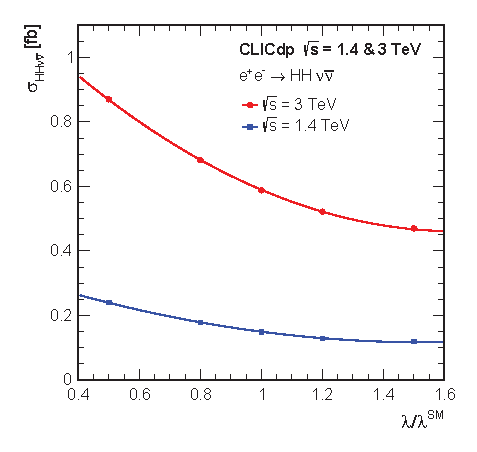
\includegraphics[width=0.45\textwidth]{{doubleHiggs/extraction/oneDrelation}}
\caption[Cross section for the \eeToHH process as a function of the ratio $\lambda/\lambda_{SM}$ ]
{Cross section for the \eeToHH process as a function of the ratio $\lambda/\lambda_{SM}$ at \rootS{1.4} and 3\,TeV, taken from \cite{Abramowicz:2016zbo}.}
   \label{fig:doubleHiggsCouplingOneDRelation}
\end{figure}


Without electron polarisation, the uncertainty on the Higgs triple self coupling $\lambda$, from  \eeToHH $\to$ \HepProcess{ \Pbottom \APbottom \PWplus \PWminus \Pnue \APnue} analysis is:
\begin{equation}
\frac{\Delta\lambda}{\lambda}=
\begin{cases}
  218\%, & \mbox{at \rootS{1.4}, }  \\
  135\%, & \mbox{at \rootS{3}}.
\end{cases}
\end{equation}

Since the Feynman diagrams for the double Higgs boson productions include t-channel $\HepProcess{\PW\PW}$-fusion, the cross section can be enhanced by using polarised electron beam. For $P(\Pem) = 80\%$, the uncertainty of  $\lambda$ becomes:
\begin{equation}
\frac{\Delta\lambda}{\lambda}=
\begin{cases}
  163\%, & \mbox{at \rootS{1.4}, }  \\
  97\%, & \mbox{at \rootS{3}}.
\end{cases}
\end{equation}
When both \sqrtS are combined, the statistical precision on \lambda increases to 99\% for the unpolarised beam, and 87\% for the polarised beam with  $P(\Pem) = 80\%$.

\section{Combined results}

When \eeToHHbbWW and \eeToHHbbbb sub-channels are combined, the expected precisions on the cross sections are:
\begin{equation}
\frac{\Delta\left[\sigma\left(\HHvv\right)\right]}{\sigma\left(\HHvv\right)}=
\begin{cases}
  44\%, & \mbox{at \rootS{1.4}, }  \\
  20\%, & \mbox{at \rootS{3}},
\end{cases}
\end{equation}

This translates to the uncertainty on the Higgs triple self coupling $\lambda$, without electron polarisation:
\begin{equation}
\frac{\Delta\lambda}{\lambda}=
\begin{cases}
  54\%, & \mbox{at \rootS{1.4}, }  \\
  29\%, & \mbox{at \rootS{3}}.
\end{cases}
\end{equation}

\section{Simultaneous couplings extraction}

The double Higgs production, \eeToHH, can occur via processes with leading Feynman diagrams shown in \Figure{fig:doubleHiggsFeynman}. As previously stated, \FIGURE{fig:doubleHiggsFeynman1} is sensitive to Higgs triple self coupling \gHHH while \FIGURE{fig:doubleHiggsFeynman2} is sensitive to quartic coupling \gWWHH. Therefore, a simultaneous extraction on the coupling uncertainty can be performed by extending the method in the \Section{sec:doubleHiggsResults}. Once a relationship between \gHHH , \gWWHH and difference in kinematic variable distributions is established, a contour of the uncertainty in \gHHH and \gWWHH two dimensional phase space can be obtained.

This two dimensional template fitting is performed at  \rootS{3}, as the precision at \rootS{1.4} is too low to support such fitting. The luminosity is assumed to be 3000$fb^{-1}$ to reflect the updated \CLIC running scenario.

The normalised cross section of the \eeToHH as a function of \gHHH and \gWWHH is shown in \Figure{fig:doubleHiggsCouplingCrossSection}. The SM cross section is normalised to 1. Around the SM coupling value, the cross section increases with the decrease of \gHHH and with the increase of \gWWHH. Hence the cross sections along the anti-diagonal are nearly constant, which would be difficult to precisely determine the statistical uncertainty on the coupling measurements.

\begin{figure}[!tbp]
    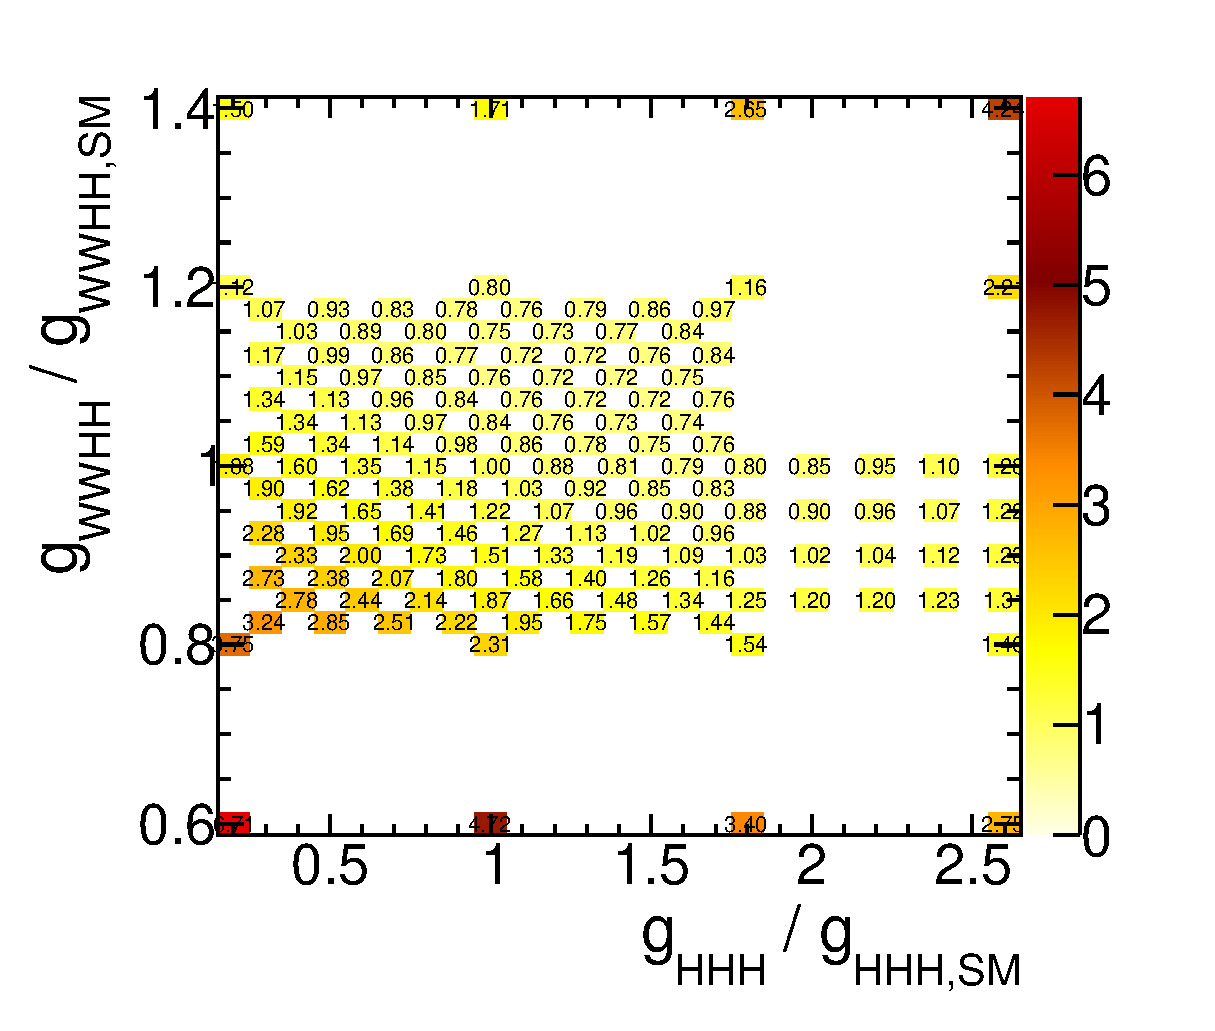
\includegraphics[width=0.85\textwidth]{{doubleHiggs/extraction/crossSectionNew}}
\caption{Normalised cross section for the \eeToHH process as a function of the $\gHHH/\gHHH_{SM}$ and  $\gWWHH/\gWWHH_{SM}$ at \rootS{3}.}
   \label{fig:doubleHiggsCouplingCrossSection}
\end{figure}

To determine the uncertainty on the coupling measurements, the variables proposed in the generator-level study in \Section{sec:theoryHiggsBSM} are used: the invariant mass of the two Higgs system, \mhh, and the sum of their transverse momenta, \HT.  %By choosing kinematic bins, high-energy behaviour can be disentailed from the physics at threshold, allowing the extraction of the coupling strength \gWWHH and \gHHH.

The strategy for coupling extraction is described below.  Simulated events with non-SM couplings are generated and reconstructed. These events went through the analysis chain discussed in this chapter with the same cuts and the same MVA classifier trained with sample of the SM coupling. The signal significance of the double Higgs events with sub-channel hadronic decay \eeToHHbbWW as a function of  \gHHH and \gWWHH is shown in \Figure{fig:doubleHiggsCouplingSignificancebbWW}.


\begin{figure}[!tbp]
    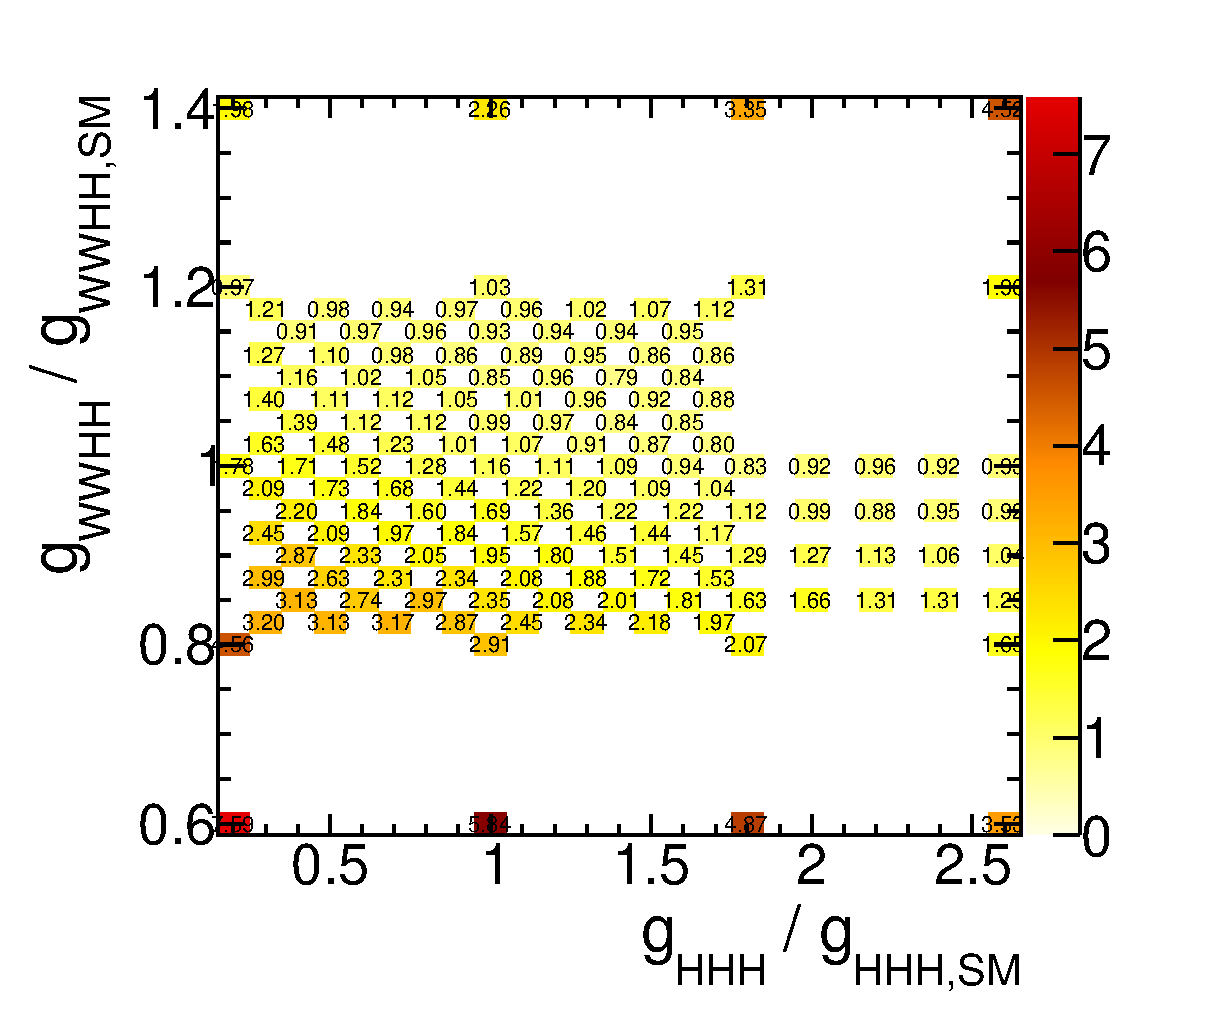
\includegraphics[width=0.85\textwidth]{{doubleHiggs/extraction/SignificanceBono}}
\caption{TODO TO UPDATE The significance for the \eeToHH process as a function of the $\gHHH/\gHHH_{SM}$ and  $\gWWHH/\gWWHH_{SM}$ at \rootS{3}, using subchannel hadronic decay \eeToHHbbWW, assuming a luminosity of  3000$fb^{-1}$.}
   \label{fig:doubleHiggsCouplingSignificancebbWW}
\end{figure}

The selected events are classified into 8 kinematic bins. 2 bins in \HT are cut at 200\,GeV. 4 bins in \mhh are cut at 500, 700, 1000\,GeV. A $\chi^2$ function is constructed to access the difference of the \mhh and \HT distributions for  non-SM coupling comparing to SM coupling sample. $\chi^2$ is:
\begin{equation}
\chi^2 = \sum_{i}^{bins}\frac{\parenths{N_i - N_{i,observed}}^2}{N_{i}},
\end{equation}
where $N_i$ is the number of event expected in a kinematic bin $i$ for a non-SM coupling sample. $ N_{i,observed}$ is the number of event observed in a kinematic bin $i$. Here the observed set can be the SM coupling sample. The expression is summing over all kinematic bins. By construction, the SM coupling point has a $\chi^2$ of 0. \FIGURE{fig:doubleHiggsCouplingChi2Separate} shows the $\chi^2$  as a function of \gHHH and \gWWHH for two sub-channels; hadronic decay \eeToHHbbWW and \eeToHHbbbb. The $\chi^2$ values for the \eeToHHbbbb sub-channel are larger due to larger signal significance obtained with this sub-channel.

\begin{figure}[!tbp]
  \begin{subfigure}[b]{0.45\textwidth}
    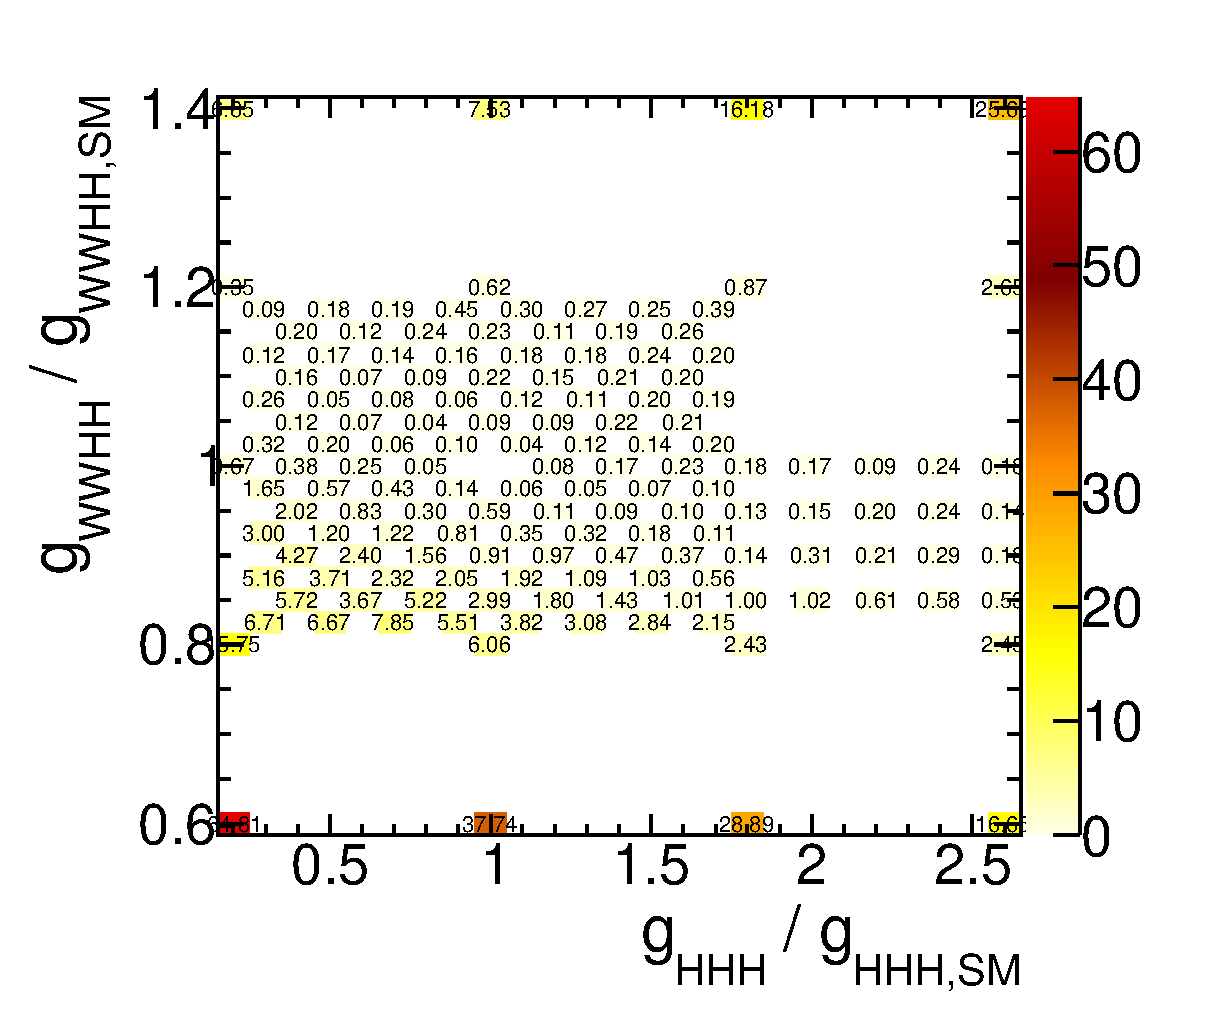
\includegraphics[width=\textwidth]{{doubleHiggs/extraction/chi2Bono4Mhh2HT}}
    \caption{\eeToHHbbWWHad, hadronic}
    \label{fig:doubleHiggsCouplingChi2bbWW}
  \end{subfigure}
    \begin{subfigure}[b]{0.45\textwidth}
    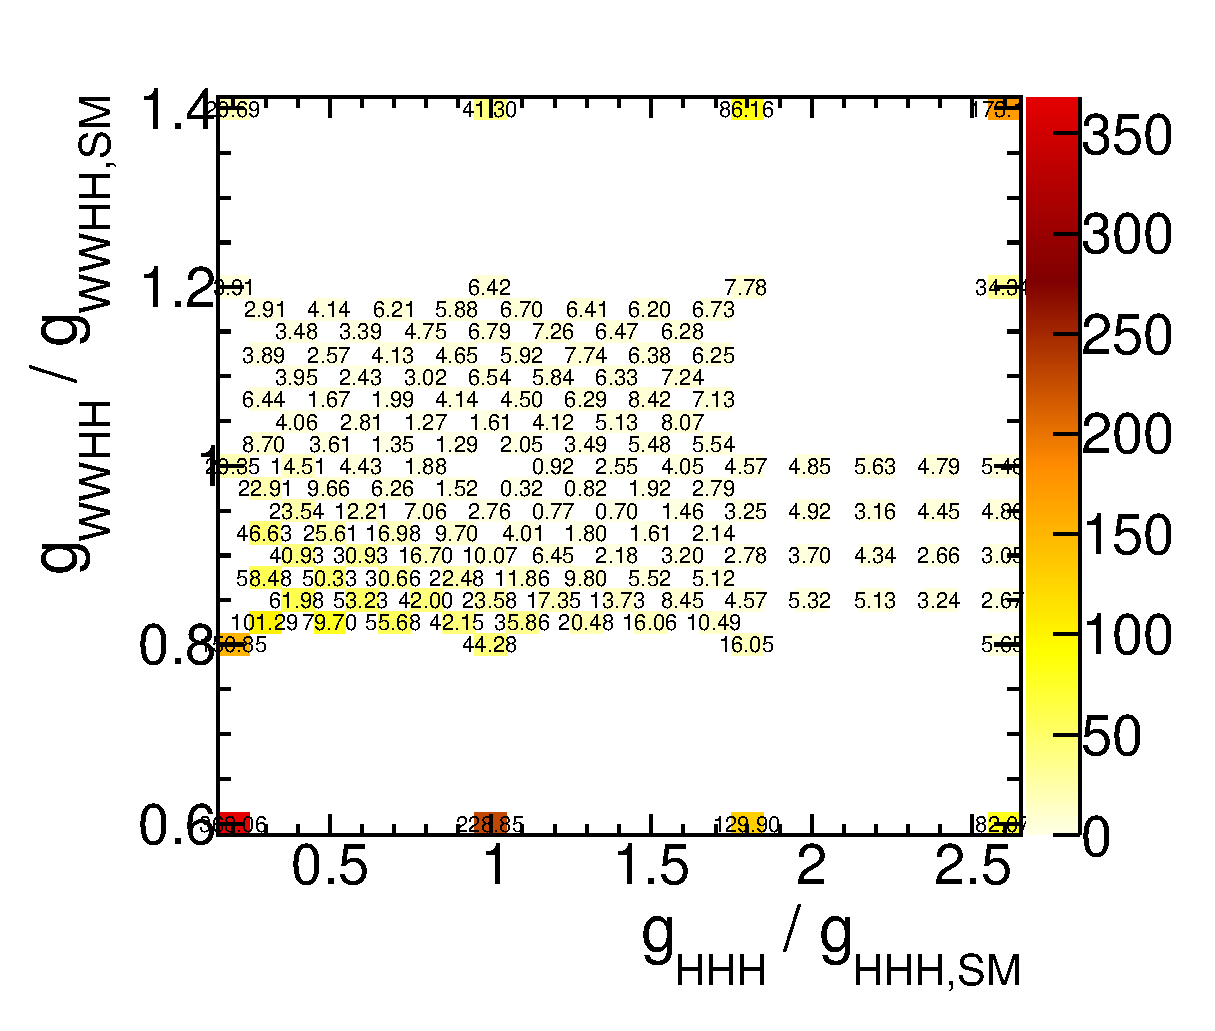
\includegraphics[width=\textwidth]{doubleHiggs/extraction/chi2Rosa4Mhh2HT}
    \caption{\eeToHHbbbb}
    \label{fig:doubleHiggsCouplingChi2bbbb}
  \end{subfigure}
\caption[$\chi^2$ as a function of $\gHHH/\gHHH_{SM}$ and  $\gWWHH/\gWWHH_{SM}$  at \rootS{3}]%
   {TODO TO UPDATE  The $\chi^2$ for the \eeToHH process as a function of the $\gHHH/\gHHH_{SM}$ and  $\gWWHH/\gWWHH_{SM}$ at \rootS{3}, using sub-channel hadronic decay \eeToHHbbWW and sub-channel, assuming a luminosity of  3000$fb^{-1}$.}
   \label{fig:doubleHiggsCouplingChi2Separate}
\end{figure}

Two sub-channels, hadronic decay \eeToHHbbWW and \eeToHHbbbb, are combined to increase the statistical precision on the coupling measurements.  Two $\chi^2$ surfaces are summed. To avoid statistical fluctuations in the sample, a toy MC experiment is performed. The SM coupling samples are treated as a data template set. 100000 data sets are generated by fluctuating the event number in each kinematic bin in the data template set according to Poisson distribution.  The $\chi^2$ is performed and summed using these generated data sets as the observed data. The summed $\chi$ is then averaged over the number of  data sets (100000) and normalised such that the $\chi^2$ at the  SM coupling is 0. Since only the difference between the non-SM and SM $\chi^2$ is used for the coupling measurements, the normalisation does not affect the measurements and helps to ease the visualisation. \FIGURE{fig:doubleHiggsCouplingChi2Ave} shows the normalised $\chi^2$ after averaging over the toy MC experiments as a function of $\gHHH/\gHHH_{SM}$ and $\gWWHH/\gWWHH_{SM}$. The $\chi^2$ changes slowly along the anti-diagonal which is similar to the cross section plot.

\begin{figure}[!tbp]
    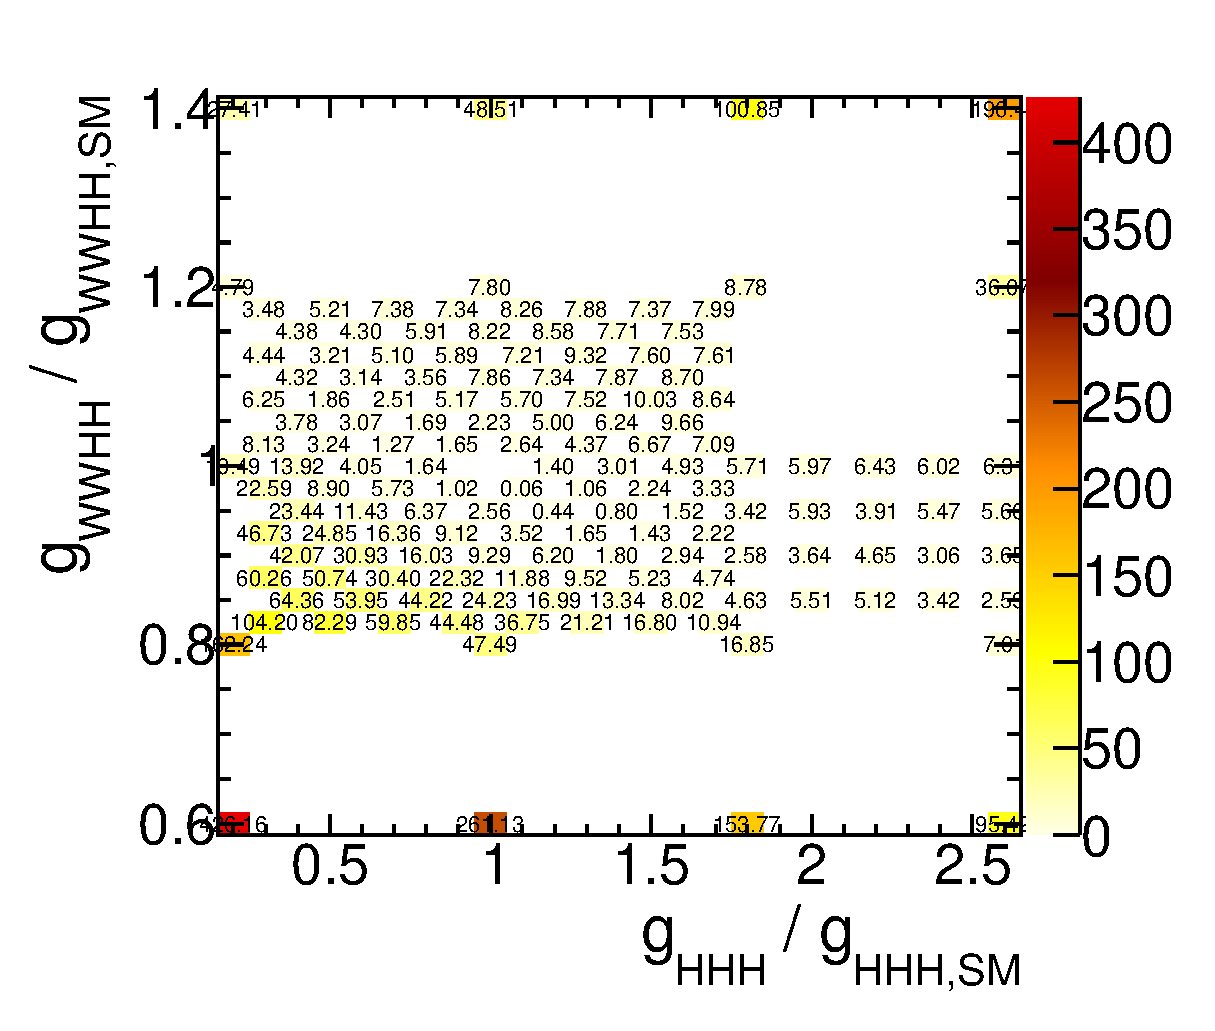
\includegraphics[width=0.45\textwidth]{{doubleHiggs/extraction/chi2Combine4Mhh2HT}}
\caption{TODO TO UPDATE  Normalised $\chi^2$, after averaging the toy MC experiments, as a function of $\gHHH/\gHHH_{SM}$ and  $\gWWHH/\gWWHH_{SM}$, combining hadronic decay \eeToHHbbWW and \eeToHHbbbb sub-channels, assuming a luminosity of  3000$fb^{-1}$.}
   \label{fig:doubleHiggsCouplingChi2Ave}
\end{figure}


\begin{figure}[!tbp]
    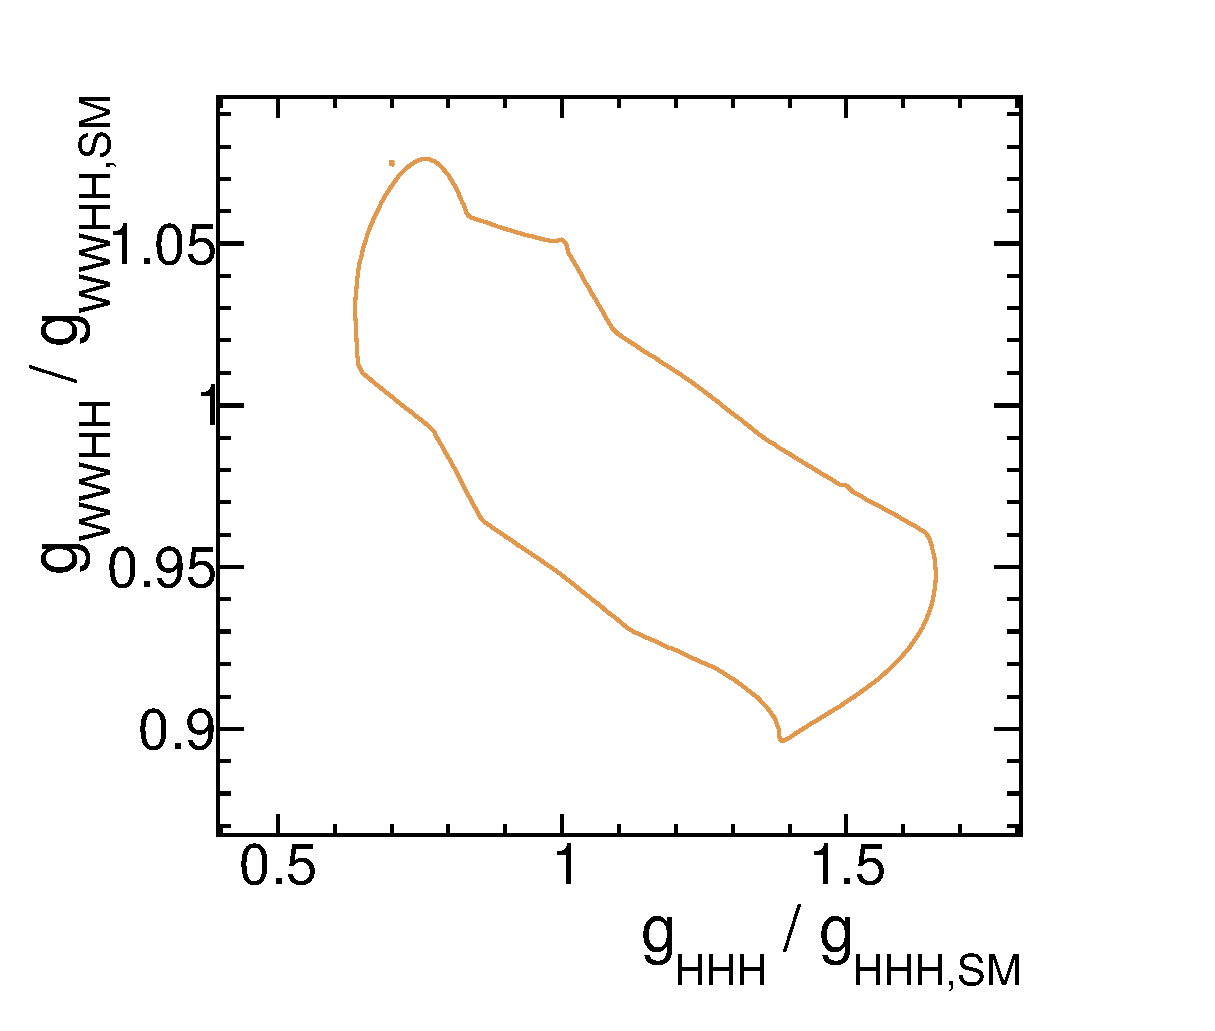
\includegraphics[width=0.45\textwidth]{doubleHiggs/extraction/chi2CombineContourLine4mHH2HTnew}
\caption{TODO Contour plot of $\chi^2$, after averaging the toy MC experiments, as a function of $\gHHH/\gHHH_{SM}$ and  $\gWWHH/\gWWHH_{SM}$,  combining hadronic decay \eeToHHbbWW and \eeToHHbbbb sub-channels, assuming a luminosity of  3000$fb^{-1}$.}
   \label{fig:doubleHiggsCouplingChi2Countour}
\end{figure}

Since there are two couplings in this $\chi^2$ surface, the degree of freedom for this fit is 2. A contour of 68\% confidence ($\chi^2 = 2.3$) can be drawn by interpolating between points on the surface. \FIGURE{fig:doubleHiggsCouplingChi2Countour} shows the contour. The counter can be sliced one dimensionally to extract the uncertainty of one coupling for a given value of the other coupling. For example:
\begin{equation}
\frac{\Delta\gWWHH}{\gWWHH} \simeq 4.9\% \text{ for \gHHH = $\gHHH_{SM}$}
\end{equation}
\begin{equation}
\frac{\Delta\gHHH}{\gHHH} \simeq 29\% \text{ for \gWWHH = $\gWWHH_{SM}$}
\end{equation}

The statistical precisions on \gWWHH and \gHHH are much better at the \CLIC than at the current \LHC or at the high luminosity upgraded \LHC \cite{Contino:2010mh}.
